\documentclass[a4paper]{report}

\usepackage{../mathstemplate}

\date{I семестр, осень 2022 г.}
\title{Алгебра. Неофициальный конспект}
\author{Лектор: Николай Александрович Вавилов \and \\ Конспектировал Леонид Данилевич}

\begin{document}

    \shorthandoff{"}
    \maketitle
    \tableofcontents
    \newpage
    \setcounter{lection}{0}


    \chapter{Введение в общую алгебру}
    \newlection{1 сентября 2022 г.}


    \section{Внутренние бинарные алгебраические операции}
    Рассмотрим произвольное множество $X \ne \o$.
    \definition[(Внутренняя) (бинарная) алгебраическая операция на $X$]{
        Отображение \[f: X \times X \map X\]
    }
    Часто операции обозначают в \emph{инфиксной} записи, например \[+: X \times X \map X; \quad(u, v) \mapsto u + v\]
    Запись выше называется \emph{аддитивной}, запись $u \cdot v$ называется \emph{мультипликативной}.

    \subsection{Частые свойства операций}
    Операции могут обладать некоторыми свойствами:
    \bullets{
        \item \emph{Коммутативность} операции $*$: $\forall x, y \in X: x * y = y * x$.
        Свойство, к которому все привыкли, но которого часто может не наблюдаться.
        Так, при отсутствии коммутативности умножения
        \[(f \cdot g)' = f' \cdot g + f \cdot g' \text{, не } f' \cdot g + g' \cdot f\]
        Или же, что, как мне кажется, невозможно угадать:
        \[\left(\frac{1}{f}\right)' = -\frac{1}{f} \cdot f' \cdot \frac{1}{f}\]
        Предположив, что $\cdot$ некоммутативно:
        \[(a + b)^2 = (a + b) \cdot (a + b) = a^2 + ab + ba + b^2\]\[(a + b)\cdot (a - b) = a^2 + ba - ab - b^2\]
        \item \emph{Ассоциативность} операции $*$: $\forall x, y, z \in X: (x * y) * z = x * (y * z)$.
        Ассоциативность намного фундаментальнее коммутативности, от неё отказаться непросто.
        Помнить про её отсутствие намного сложнее, чем про отсутствие коммутативности.

        Практически все структуры, которые мы будем рассматривать, будут ассоциативны.

        Ассоциативность и коммутативность абсолютно независимы, каждая может как выполняться, так и нет, вне зависимости от другой.

        \item \emph{Дистрибутивность} $*$ относительно $+$: $x * (y + z) = (x * y) + (x * z)$.
        Дистрибутивность выполняется для двух операций, здесь $*$ дистрибутивна относительно $+$.
        Так, для целых чисел $a \cdot (b + c) = a \cdot b + a \cdot c$.

        \emph{Самодистрибутивность}: $x * (y * z) = (x * y) * (x * z)$.
        Очень необычное свойство, с которым неожиданно связаны парадоксальные результаты.
        Так, есть вполне конкретно определённая конечная группа (в которой выполняется самодистрибутивность), для которой истинность некоторого факта (о порядке некоего элемента) зависит от существования больших кардиналов.
        Всё, что могут просчитать компьютеры, не превосходит 16, но в предположении существования больших кардиналов эта величина может быть сколь угодно большой при больших конечных группах этого типа.
    }
    \emph{
        На лекции приводилось определение композиции внутренних функций, действующих из множества в него само: $f \in X^X$.
        Мне захотелось, поэтому я привёл определение и доказательство более общей композиции, которая, впрочем, от этого перестала быть внутренней операцией.
    }
    \definition[Композиция]{
        Отображение, результат которого --- последовательное применение двух.
        Формально, для функций $f: B \map C$ и $g: A \map B$ композиция определяется, как отображение $f \circ g: A \map C; \quad (f \circ g)(x) = f(g(x))$.

        Композиция --- внешняя операция (внутренняя для $A = B = C$):\quad  $\circ: C^B \times B^A \map C^A$.
    }
    \theorem{\label{composition_associativity}Композиция ассоциативна: $(f \circ g) \circ h = f \circ (g \circ h)$.
    \provehere{
        Отображения совпадают, если совпадают их области определения, области значений, а также значения во всех точках области определения.

        Пусть $f: E \map F; \quad g: C \map D; \quad h: A \map B$.

        $\exists f \circ g \iff D = E;\quad \exists (f \circ g) \circ h \iff B = C$.
        Аналогично, $\exists f \circ (g \circ h) \iff B = C \land D = E$.

        Таким образом, левая часть существует, если и только если существует правая --- ассоциативность \emph{строгая}.

        Кроме того, $(f \circ g) \circ h: A \map F$ и $f \circ (g \circ h): A \map F$.

        Наконец, удостоверимся, что совпадают значения во всех точках области определения $A$.
        \[((f \circ g) \circ h)(x) = (f \circ g)(h(x)) = f(g(h(x))) = f((g \circ h)(x)) = (f \circ (g \circ h))(x)\]

        Все четыре знака равенства используют только определение композиции.
    }}

    \note{
        В формуле выше, как и во всех правильно написанных формулах, от равенства к равенству не меняется порядок переменных --- в данном случае это $f, g, h, x$.
    }
    \theorem{
        Из ассоциативности следует обобщённая ассоциативность.
        А именно, в формуле $x_1 \circ x_2 \circ \dots \circ x_n$ можно как угодно (корректно) расставить скобки, при ассоциативной операции $\circ$ результат не изменится.
        \provehere{
            Доказательство по индукции.

            \underline{База:} $n \le 2$ --- всего один вариант расстановки скобок.
            $n = 3$ --- определение ассоциативности.

            \underline{Переход:} докажем, что при любой расстановке скобок выражение можно привести к левонормированной форме: форме \[(((x_1 \circ x_2) \circ x_3) \dots) \circ x_n\]
            Рассмотрим последнюю переменную $x_n$. Возможны два случая:
            \bullets{
                \item $\circ$, принимающий в качестве правого аргумента $x_n$, в качестве левого аргумента принимает некое выражение от $x_1, \dots, x_{n-1}$.
                Тогда, применив предположение индукции, мы можем считать, что левый аргумент --- левонормированная форма $((x_1 \circ x_2) \dots) \circ x_{n - 1}$.

                В таком случае всё выражение тоже оказалось левонормированным.
                \item $\circ$, принимающий в качестве правого аргумента $x_n$, в качестве левого аргумента принимает выражение от переменных $x_i, \dots, x_{n - 1}~(i > 1)$.
                Так как $i > 1$, то мы можем применить индукционное предположение к переменным $x_i, \dots, x_n$.
                Теперь эта часть формулы левонормированная: $(\dots) \circ (((x_i \circ x_{i + 1}) \dots) \circ x_n)$.
                Воспользуемся ассоциативностью, получим $((\dots) \circ (((x_i \circ x_{i + 1}) \dots)) \circ x_n$.
                Таким образом, задача свелась к предыдущему случаю. \qedhere
            }
        }
    }
    \newlection{7 сентября 2022 г.}

    \subsection{Примеры внутренних бинарных алгебраических операций}
    \label{binary_operations}
    \begin{itemize}
        \item Над числами
        \item Сумма многочленов
        \item Произведение многочленов
        \item Композиция многочленов.
        $(x + 1) \circ x^2 = x^2 + 1$, в то время как $x^2 \circ (x + 1) = (x + 1)^2$, откуда видно, что композиция некоммутативна.
        \item \emph{Кронекеровская сумма}.
        Определим её для простоты над нормированными многочленами $f, g$ (старший коэффициент $1$).
        $f \boxplus  g$ --- нормированный многочлен, корни которого $\alpha_i + \beta_j$ для всех $\alpha_i$ --- корней $f$, $\beta_j$ --- корней $g$.

        \item \emph{Кронекеровское произведение}.
        Определим его для простоты над нормированными многочленами $f, g$ (старший коэффициент $1$).
        $f \boxtimes  g$ --- нормированный многочлен, корни которого $\alpha_i \cdot \beta_j$ для всех $\alpha_i$ --- корней $f$, $\beta_j$ --- корней $g$.

        \item Над векторами.
        Будем обозначать вектор $\begin{pmatrix}
                                     x_1\\ \vdots \\ x_n
        \end{pmatrix}$ или $\begin{pmatrix}
                                x_1& \cdots & x_n
        \end{pmatrix}$.
        Обе записи валидны, но отличаются левым и правым действием.
        Тогда $\begin{pmatrix}
                   x_1\\ \vdots \\ x_n
        \end{pmatrix} + \begin{pmatrix}
                            y_1\\ \vdots \\ y_n
        \end{pmatrix} = \begin{pmatrix}
                            x_1 + y_1\\ \vdots \\ x_n + y_n
        \end{pmatrix}$.

        \item Скалярное умножение векторов (покомпонентное)  $\begin{pmatrix}
                                                                  x_1\\ \vdots \\ x_n
        \end{pmatrix} \cdot \begin{pmatrix}
                                y_1\\ \vdots \\ y_n
        \end{pmatrix} = \begin{pmatrix}
                            x_1 \cdot y_1\\ \vdots \\ x_n \cdot y_n
        \end{pmatrix}$.

        \item Комплексное умножение векторов $\vect{a, b} \cdot \vect{c, d} = \vect{ac - bd, ad + bc}$.

        \item Векторное умножение в трёхмерном пространстве $\vect{x_1, x_2, x_3} \times \vect{y_1, y_2, y_3} =  \vect{x_2 y_3 - x_3 y_2\\-x_1 y_3+x_3 y_1\\x_1 y_2-x_2 y_1}$.

        \item Операции над матрицами.
        Рассмотрим матрицы $2 \times 2$ с коэффициентами из $R$, где

        $R \in \{\Z, \Q, \R, \dots \}$.
        Обозначается $M(2, R) = \defset{\vect{a &b\\c & d}}{a, b, c, d \in R}$.

        Сложение: $\vect{a&b\\c&d}+\vect{e&f\\g&h}=\vect{a+e&b+f\\c+g&d+h}$.

        \item Умножение матриц по Шуру (по Адамару) $\vect{a&b\\c&d} \odot \vect{e&f\\g&h}=\vect{a\cdot e&b\cdot f\\c\cdot g&d\cdot h}$.
        \item Настоящее умножение матриц: $\vect{a&b\\c&d}\cdot\vect{e&f\\g&h}=\vect{a\cdot e + b \cdot g&a\cdot f + b \cdot h\\c\cdot e + d \cdot g&c \cdot f + d \cdot h}$

        \item Булевы операции (на булеане) --- пересечение, объединение, т.\ д.,\ т.\ п..
    \end{itemize}


    \section{Простейшие структуры. Моноиды}

    Моноид состоит из множества $X \ne \varnothing$ и операции $* : X \times X \map X;\quad (x, y) \mapsto x * y$.
    Операцию можно ввести кучей ($|X|^{|X|^2}$) способов, но мы будем рассматривать операцию, удовлетворяющую каким-то тождествам.

    \subsection{Полугруппа (semi-group)}

    Операция $*$ ассоциативна.

    \subsection{Моноид}
    \begin{itemize}
        \item M1: Множество --- полугруппа, т.\ е.\ операция $*$ ассоциативна.
        \item M2: Существует нейтральный элемент $e \in X: \forall x \in X : e * x = x * e = x$.
        В аддитивной нотации обозначается $0$, в мультипликативной используют $1$.

        \note{Если существует и левый, и правый нейтральные элементы, то они совпадают: $e = e * e' = e'$.}
    \end{itemize}

    \subsubsection{Примеры моноидов}
    Ниже указаны моноиды в виде $(\cdots, \cdots, \cdots)$ --- запись \emph{сигнатуры}.
    В сигнатуру моноида входит множество, операция, нейтральный элемент.
    \bullets{
        \item $(\N, \cdot, 1)$.
        \item $(\N_0, +, 0)$.
        \item $X = 2^Y \quad (X, \cup, \varnothing) \quad (X, \cap, Y)$.
        \item Симметрический моноид: $(X^X, \circ, \id_X)$ -- множество всех преобразований множества $X$ в себя.

        Я просто запишу эти крестики здесь: $X^X \times X^X \map X^X, (f, g) \mapsto g \circ f$
    }

    \subsubsection{Определения}
    \definition [$z \in X$ регулярен]{
        $\begin{cases}
             \forall x, y \in X: ((x * z = y * z) \then x = y) &\text{ --- регулярен справа}\\
             \forall x, y \in X: ((z * x = z * y) \then x = y) &\text{ --- регулярен слева}
        \end{cases}$
    }

    \definition[Обратимый слева / справа элемент]{
        Элемент $z \in X$ называется обратимым слева $\iff \exists u \in X : u * z = e$.
        Аналогично, $z$ обратим справа $\iff \exists v \in X: z * v = e$.}

    \lemma{ $z$ обратим слева / справа $\then z$ регулярен слева / справа.}

    \provehere{
        $\exists u \in X : u * z = e$. Тогда если $z * x = z * y$, то --- умножив на $u$ слева --- $(u * z) * x = (u * z) * y$ и $x = y$.
    }

    \definition[Обратимый элемент]{Элемент $z \in X$ называется обратимым $\iff \exists u \in X : u * z = z * u = e$. В таком случае $u$ --- обратный (противоположный, симметричный, ...) к $z$.}

    \lemma{
        \label{inversability}
        В моноиде $z$ обратим слева и справа $\iff z$ обратим.
        \provehere{
            Рассмотрим обратные к $z$ слева $u_L$ и справа $u_R$.
            Запишем произведение \[u_L = u_L * (z * u_R) = (u_L * z) * u_R = u_R\qedhere\]
        }
    }
    Пусть $X^* = \defset{z \in X }{~ \exists z^{-1} \in X : z^{-1}*z = e = z * z^{-1}}$ --- множество обратимых элементов моноида $(X, *)$.

    \begin{itemize}
        \item $e \in X^*$.
        \item $x, y \in X^* \then (x * y)^{-1} = y^{-1} * x^{-1}$.
        \item $x \in X^* \then x^{-1} \in X^*$
    \end{itemize}

    \corollary{$X^*$ --- группа обратимых элементов моноида $X$.}


    \section{Группы}

    Пусть $G$ -- множество; $* : G \times G \map G$.

    \definition[Группа]{$(G, *)$ -- группа:
        \begin{itemize}
            \item M1. $*$ ассоциативна
            \item M2.  $\exists e \in G:(\forall x \in G:)~ e * x = x * e = x$.
            \item M3. Все элементы обратимы: $\forall g \in G: \exists g^{-1} \in G : g * g^{-1} = g^{-1} * g = e$.
        \end{itemize}
    }

    Группа $G$ называется коммутативной (или абелевой), если $*$ коммутативна.
    В абелевых группах принята аддитивная запись: $(*, 1, x^{-1}) \rightsquigarrow (+, 0, -x)$

    В сигнатуру группы входят 4 вещи: $(G, *, e, {}^{-1})$, где ${}^{-1} : G \map G; x \mapsto x^{-1}$.

    \newlection{8 сентября 2022 г.}
    \lemma{
        В любой группе $G$ есть деление:
        $\switch {
            \forall h, g \in G : \exists!~ x:~h*x = g \text{ --- левое деление}\\
            \forall h, g \in G : \exists!~ y:~x * y = g \text{ --- правое деление}
        }$
    }
    \begin{proof}
        $x = h^{-1}g$ в случае левого деления;
        в случае правого деления $y = g^{-1}h$.
    \end{proof}

    \note{Для большинства свойств группы достаточно более слабого, нежели $g*g^{-1} = e$, а именно, часто достаточно $gg^{-1}g = g$.}

    \subsection{Примеры групп}
    Абелева (коммутативная) группа --- на самом деле не группа (формально группа, но морально --- совсем не так).
    \examples[Группы] {
        \item Какая-то группа симметрий, преобразований на себя. Например, повороты кубика Рубика.
        Нейтральный элемент --- не делать поворотов.
        \item Пусть $(R, +, \cdot, 0)$ --- кольцо.
        Аддитивная группа кольца, группа по сложению $R^+ = (R, +, 0)$.
        Например, для кольца $\Z: \Z^+ $ --- бесконечная циклическая группа.
        Аналогично получаются $\R^+, \Q^+$, однако стоит упоминания, что $\Q, \R$ --- это уже поля.
        \note {
            Операции деления и вычитания рассматриваются не как самостоятельные, а как производные операции, поэтому не записываются в сигнатуре.
            Так, $x - y = x + (-y)$.
        }
        \item Пусть $R$ --- ассоциативное кольцо с единицей. Тогда его мультипликативная группа $R^* = \defset{ x \in R }{~ \exists y \in R : xy = 1 = yx}. \quad Z^* = \{-1, 1\}.\quad \Q^* = \Q \sm \{0\};\quad \R^* = \R \sm \{ 0 \}$.

        \item Группа углов $\mathbb{T} = \bigdefset{ z \in \C }{ |z| = 1} \cong \R / 2\pi\Z$.

        \definition[Подгруппа] {
            $H \ne \varnothing; H \subset G: H$ называется подгруппой в $G$, если

            $\forall x, y \in H:
            \left(xy^{-1} \in H \overset{\text{здесь равносильно}}{\iff} \switch {
                xy \in H \\
                y^{-1} \in H
            }\right)$. Пишут ${(H \le G) \iff (H\text{ --- подгруппа }G)}$.
        }
        \item $\R_{>0} < \R^*$

        $\Q_{>0} < \Q^*$

        \item Группа корней $n$-й степени ($n \in \N$) из единицы $M_n = \defset{ z \in \C^* }{ z^n = 1 } < \mathbb{T}$.
        $|M_n| = n$.

        \definition[Степень в моноиде] {
            Пусть $X$ --- моноид с нейтральным элементом $e$. $x \in X; \quad n \in \N_0$.
            Тогда $n$-я степень $x$: $x^n = \switch{ e,& n = 0 \\ x^{n-1}*x,&n \ge 1}$.

            \note {
                Почему-то лектор настаивает на определении $x^n = \switch{ e,& n = 0 \\ \left(x^{\frac{n}{2}}\right)^2,&2 \divs n \\ x^{n-1}*x,&2 \notdivs n}$

                Однако я бы предпочёл это держать свойством.
            }
        }

        \definition[Степень в группе] {
            Пусть $X^*$ --- мультипликативная группа моноида $X$ с нейтральным элементом $e$. $x \in X; \quad n \in \Z$.
            Тогда $n$-я степень $x$: $x^n = \switch{ x^n,& n \ge 0 \\ \left(x^{-1}\right)^{-n},&n < 0}$.
        }
        \item <<Настоящая>> (некоммутативная) группа: $S_X = \Bij(X, X)$ --- симметрическая группа множества $X$.
        Эквивалентно множеству обратимых элементов симметрического моноида $X^X$.

        \note {
            Частный случай --- $X = \underline{n} = \{1, 2, \dots n \}$. Симметрическая группа $S_n \bydef S_{\underline{n}}$. Как известно, $|S_n| = n!$.
        }
        Записывается $S_3$ следующим образом:

        $\left\{\vect{1&2&3\\1&2&3}, \vect{1&2&3\\1&3&2}, \vect{1&2&3\\2&1&3}, \vect{1&2&3\\2&3&1}, \vect{1&2&3\\3&1&2}, \vect{1&2&3\\3&2&1}\right\}$.

        В верхней строчке перечислены элементы $X$, в нижней, соответственно --- их образы при применении данного элемента.
        Так, для перестановки $p$ образ $i$ обозначается $p(i)$ или $p_i$.

        Перемножение:
        $(p \cdot q)_i = p_{q_i}$. Перемножение, как композиция, считается справа налево.
        Некоммутативность перемножения:

        $\vect{1&2&3\\2&1&3} \cdot \vect{1&2&3\\2&3&1}=\vect{1&2&3\\1&3&2}$

        $\vect{1&2&3\\2&3&1} \cdot \vect{1&2&3\\2&1&3}=\vect{1&2&3\\3&2&1}$
        \item Группа обратимых линейных операторов $GL(n, R)$.

        В кольце матриц $M(n, R)$ существует нейтральный элемент: $e = \vect{1&0\\0&1}$ в случае $M(2, R)$. $GL(n, R) \bydef M(n, R)^*$ --- полная линейная группа степени $n$ над $R$. Например, для поля $K: GL(2, K) = \defset{ \vect{a&b\\c&d}}{a,b,c,d\in K \land ad - bc \ne 0}$. В самом деле, $\vect{a&b\\c&d}^{-1}=\dfrac{1}{ad-bc}\vect{d&-b\\-c&a}$.

        \item Размер (мощность множества) конечной группы называют \emph{порядком} группы.

        Как устроены группы маленьких (конечных) порядков?
        \numbers {
            \item $|G| = 1$. Здесь $G = \{1\}$.
            \item \up \definition {
                Для $n \in \N:~ \exists~ C_n \cong M_n$ --- группа вращений правильного $n$-угольника. $C$ от слова cyclic --- циклическая группа.
            }
            \item $|G| \in \P$. Существует только циклическая группа такого размера! $C_{|G|}$
            \item $|G| = 4$. Такого размера есть группы $C_4, C_2 \times C_2$.
            \definition[Прямое произведение групп] {
                $H \times G = \{(h, g) | h \in H, g \in G\}$.
                Умножение определяется $(h_1, g_1) \cdot (h_2, g_2) = (h_1 h_2, g_1 g_2)$.
            }
            \item $|G| = 6$. Группы такого размера бывают двух типов: $C_6 = C_2 \times C_3; S_3 \cong D_3$.
            \definition[Диэдральная группа] {
                $D_n$ --- группа симметрий (включающих отражение) правильного $n$-угольника. $|D_n| = 2n$.
                \newlection{14 сентября 2022 г.}
                $D_2 \cong V; D_3 \cong S_6$. $V$ --- группа симметрий квадрата, получаемых отражением относительно диагоналей.
            }
            \item $|G| = 8 \then \dots$. Для составных $n$ задача определения по порядку группы её возможные типы --- сложная.

            Существует 5 групп порядка $8$:
            \bullets{
                \item $C_8$ --- циклическая группа.
                \item $C_2 \times C_4$
                \item $C_2 \times C_2 \times C_2$
                \item $D_4$ --- диэдральная группа. Не является абелевой!
                \item $Q_8 =\{\pm 1, \pm i, \pm j, \pm k\}$ --- группа кватернионных единиц. (\textbf Quaternion). Не является абелевой группой!

                Кватернионы, натянутые на эти 4 единицы определяют четырёхмерное пространство; ещё Гамильтон за 60 лет до появления теории относительности писал, что 1 отвечает за временную одномерную ось, а $i, j, k$ --- векторы трёхмерного пространства.

                Кватернионы $\mathbb{H} \bydef \defset{a + bi + cj + dk}{a, b, c, d \in \R}$, где $i, j, k$ --- мнимые единицы, удовлетворяющие тождествам $i^2 = j^2 = k^2 =ijk = -1$ и $xy = -yx$. Ассоциативность проверяется грубой силой с большими затратами, или же специальными матрицами $M(2, \C)$ --- матрицами Паули.}

            \definition[Порядок элемента $g$ в группе $G$]{Наименьшее натуральное $n \in \N: g^n = 1_G$. }
            \note{В различности данных пяти групп можно убедиться, заметив различие мультимножеств порядков их элементов.}

            Описание групп больш$\acute{\text{и}}$х составных порядков --- сложная задача.

            Задача 2000 --- описать все группы порядка $\le 2000$ до наступления нового века. Задача практически была решена, не удалось лишь перечислить $~ 5 \cdot 10^{10}$ групп порядка 1024, составляющие больше $99\%$ всех групп порядка менее $2000$.

        }
    }

    \subsection{Гомоморфизмы}
    Рассмотрим множество $X$ с операцией $*$ и множество $Y$ с операцией $\circ$.
    \definition[Гомоморфизм]{
        Отображение $f: X \map Y$, такое, что \[\forall x, y \in X : f(x) \circ f(y) = f(x*y)\]
    }

    \subsubsection{Примеры гомоморфизмов}
    \bullets {
        \item Экспонента. $\exp : \R^+ \map \R_{>0}^*; \quad x \mapsto e^x$.

        \emph{Напоминание: $\R^+ = (\R, +, 0)$; $R^*_{>0} = (\R_{>0}, \cdot, 1)$.}
        \item Логарифм $\log : \R_{>0}^* \map \R^+; \quad x \mapsto \log(x)$.

        $\log(\exp(x)) = x \quad \exp(\log(x)) = x$

        \definition[Изоморфизм]{
            Обратимый гомоморфизм (обратный к которому --- тоже гомоморфизм).
            Часто это то же самое, что и биективный гомоморфизм, но не всегда.
            Так, если к гомоморфизму есть требование непрерывности, то обратный гомоморфизм тоже обязан не только существовать, но и быть непрерывным.
        }

        \definition[Изоморфные множества $X \cong Y$]{
            Между ними существует изоморфизм.
        }

        \note{
            Важным свойством $\R$ является $\R^*_{>0} \cong \R^+$, что, например, не выполнятся ни для $\Q$, ни для $\mathbb{A}$.
        }

        \item Абсолютная величина. $|\cdot|: \R \map \R_{\ge 0}; \quad x \mapsto |x|$.

        \emph{Мультипликативный гомоморфизм} по умножению.

        \item Знак. $\sign : \R^* \map \{\pm 1\}; \quad \sign(x) = \switch{+1,&x > 0\\ -1,& x < 0}; \quad \sign(x \cdot y) = \sign(x) \cdot \sign(y)$

        \note{
            $\left(x = \sign(x) \cdot |x|\right) \then \R^* \cong \left(\R_{>0} \times \{\pm 1\}\right)$
        }

        \item $\C^* \cong \R^*_{>0} \times \mathbb{T}$ --- модуль и аргумент.
        В школе этот факт гомоморфизма называется теоремой сложения для синусов и косинусов.

        \note{
            Также наблюдается гомоморфизм

            $\mathbb{T} \map M(2, \R); \quad x \mapsto \vect{\cos(x) &\sin(x)\\ -\sin(x)&\cos(x)}$.

            В матрицах тригонометрические формулы:

            $\vect{\cos(x) &\sin(x)\\ -\sin(x)&\cos(x)} \cdot \vect{\cos(y) &\sin(y)\\ -\sin(y)&\cos(y)} = \vect{\cos(x+y) &\sin(x+y)\\ -\sin(x+y)&\cos(x+y)}$ --- ф-ла А. де Муавра.
        }
        \intfact[Коан]{
            $\C^* \cong \T$.
        }
        \item Знак перестановки.
        $\sgn: S_n \map \{\pm 1\}$. Можно определить его, как количество инверсий --- пар позиций $i < j: p_i > p_j$.

        Так $\sgn\vect{1&2&3\\2&1&3} = -1, \quad \sgn\vect{1&2&3\\2&3&1} = +1$.
        Знак перестановки --- мультипликативный гомоморфизм.

        \item Определитель (детерминант) --- $\det : M(n, \R) \map \R$.

        Если ввести определитель только от обратимых матриц: $\det: GL(n, \R) \map \R^*$, то тоже получится мультипликативный гомоморфизм.

        \item Аддитивный гомоморфизм взятия производной: $(f + g)' = f' + g'$.
    }

    \definition[Гомоморфизм моноидов]{
        $f : X \map Y$ --- гомоморфизм моноидов, если \[\forall x, y \in X : f(xy) = f(x)f(y)\text{ и }f(1_X) = 1_Y\]
    }
    \definition[Гомоморфизм групп]{
        $f : H \map G$ --- гомоморфизм групп, если \[\forall x, y \in X : f(xy) = f(x)f(y)\]
    }

    \note{
        Сигнатура моноида: $(X, \cdot, 1)$. Сигнатура группы: $(G, \cdot, 1, \inv)$.
        По-хорошему, в определение гомоморфизма групп надо включить сохранение единицы и обратного, но

        \lemma{
            Если $f : H \map G$ --- мультипликативный гомоморфизм для групп $H, G$, то автоматически $f(1_H) = 1_G$ и $f(x^{-1}) = f(x)^{-1}$.
            \provehere{
                $1_H \cdot 1_H = 1_H \then f(1_H) = f(1_H \cdot 1_H) = f(1_H)^2$.
                Так как $G$ --- группа, то можно сокращать.
                Поэтому $f(1_H) = 1_G$.
                Тогда сохраняется и обратный: $1_G = f(1_H) = f(xx^{-1}) = f(x)f(x^{-1})$, откуда в силу единственности обратного $f(x^{-1}) = f(x)^{-1}$.
            }
        }
        \note{
            Для моноидов лемма неверна, так как, например, существует отображение $\{1\} \map M$, где $1 \mapsto x$, $x$ --- произвольный идемпотент в моноиде $M$. Оно не является гомоморфизмом, хотя для него выполняется <<правило умножения>>.
        }
    }


    \section{Дистрибутивность, определение кольца.}
    Пусть $(X, *, \circ)$ --- произвольное множество с двумя операциями.

    \definition[Дистрибутивность]{$*$ дистрибутивна слева относительно $\circ$, если

        $\forall x, y, z \in X : x * (y \circ z) = (x * z) \circ (x * z)$ и дистрибутивна справа, если $(x \circ y) * z = (x * z) \circ (y * z)$.}
    \note{Для коммутативной операции $*$ говорят только просто о дистрибутивности. }

    \subsection{Примеры дистрибутивных операций}
    \bullets{
        \item Обычно $x \cdot (y + z) = x \cdot y + x \cdot z$ и $(x + y) \cdot z = x \cdot z + y \cdot z$.
        \item Булевы операции $\cap, \cup$ --- каждая коммутативна и дистрибутивна относительно другой.
        \item \up \definition[Самодистрибутивность]{$*$ --- самодистрибутивна слева, если $x * (y * z) = (x * y) * (x * z)$. Аналогично справа. }
    }
    \newlection{15 сентября 2022 г.}

    \subsection{Кольцо}
    \definition[Кольцо]{Кольцо --- множество $R \ne \varnothing$ с двумя операциями $+$ и $\cdot$ --- сложение и умножение. Операции такие, что:
    \bullets{
        \item A: $(R, +)$ --- абелева (коммутативная) группа.
        \numbers{
            \item $(x + y) + z = x + (y + z)$.
            \item $\exists 0 \in R: x + 0 = 0 + x = x$.
            \item $\forall x \in R : \exists -x \in R : x + (-x) = 0 = (-x) + x$.
            \item $x + y = y + x$. \note{В кольцах с единицей коммутативность сложения автоматически следует из дистрибутивности.}
        }
        \item D: $\cdot$ двусторонне дистрибутивно относительно $+$.
        \numbers{
            \item $a \cdot (b + c) = a \cdot b + a \cdot c$
            \item $(a + b) \cdot c = a \cdot c + b \cdot c$
        }
    }}

    \subsection{Примеры колец}
    \bullets{
        \item Кольцо Ли, умножение неассоциативно: $V = \R^3$, сложение --- сложение векторов, умножение --- умножение векторов.
        \note{
            В таком кольце выполняется \emph{тождество Як$\acute{\text{о}}$би}: $(xy)z + (yz)x + (zx)y = 0$ и тождество антикоммутативности $x^2 = 0\overset{\text{из раскрытия $(x + y)^2$}} {\then} xy = -yx$.}
        \note{
            Тождество Якоби примерно аналогично \emph{тождеству Лейбница}: $D(f\cdot g) = D(f)\cdot g + f\cdot D(g)$.
        }
        \note{
            Часто используют \emph{алгебру} Ли вместо кольца Ли, в алгебре можно ещё умножать на скаляр.
        }
        \note{
            На начальном этапе все рассматриваемые кольца будут ассоциативны.
        }
        \definition[Ассоциативное кольцо]{$x\cdot(y\cdot z) = (x \cdot y) \cdot z$.
        }
        \definition[Кольцо с единицей (унитальное кольцо)]{
            Выполняется аксиома M2: все элементы образуют мультипликативный моноид: $\exists 1 \in R: x\cdot 1 = 1 \cdot x = x$.
        }

        \definition[Коммутативное кольцо]{
            Умножение коммутативно.
            Часто подразумевают, что коммутативное кольцо ассоциативно, но это не следует ниоткуда.
        }

        \note{
            Коммутативность влечёт $(x - y)(x + y) = x^2 - y^2$. Без неё \[(x - y)(x + y) = x^2 + xy - yx - y^2 = x^2 + [x, y] - y^2\] где $[x, y] \bydef xy - yx$ --- коммутатор $x, y$.
            Аналогично \[(x + y)^2 = x^2 + 2(x \circ y) + y^2\]где $x \circ y \bydef \frac{1}{2}(xy + yx)$ --- антикоммутатор.
        }
        \note{Верно для произвольного ассоциативного кольца:
        \bullets{\item $0 \cdot x = 0$. \item $(x - y)z = xz - yz$, где $x - y = x + (-y)$. \item $(-x)(-y) = xy$.}}
        \definition[Тело]{
            $R$ --- тело, если $R$ --- ассоциативное кольцо с единицей и выполняется М4: $\forall x \in R \sm \{0\}: \exists x^{-1} \in R : xx^{-1} = x^{-1}x = 1$
        }
        \definition[Поле]{
            Коммутативное тело, т. е. тело с коммутативным умножением.
            Часто обозначается $K$ или $F$.
            Выполняются аксиомы А1 -- А4, D1, D2, M1 -- M4, $1 \ne 0$.
        }

        \item Нулевое кольцо: $0 = 1 \then 0 = 0 \cdot x = 1 \cdot x = x$. Кольцо из одного элемента.
        \item Некольцо: Рассмотрим множество многочленов с коэффициентами из $K$: $K[x]$.

        $+$ --- сложение многочленов.

        $\cdot$ --- композицию многочленов.

        Заметим, что $(f + g) \circ h = f\circ h + g \circ h$, но структура --- не кольцо, так как $f \circ (g + h) \ne f \circ g + f \circ h$.
        \item Здесь и далее: коммутативные ассоциативные кольца с единицей.

        Кольцо целых чисел $\Z$. Это коммутативное ассоциативное кольцо с единицей без делителей нуля.

        $\R, \Q, \C$ --- поля.

        \item Булевы кольца. Определим их на булеане множеств. $R = 2^X$.

        $\cdot$ --- $\cap$.

        $+$ --- ? ($\cup$ брать нельзя, так как нет противоположного). $+$ --- $\triangle$ (симметрическая разность).

        Пример булевого кольца над синглетоном: $\mathbb{F}_2 \bydef \{0; 1\}$.

        Таблицы Кэли для $\mathbb{F}_2$:
        \begin{table}[!ht]
            \centering

            \begin{tabular}{c | c c}
                + & 0 & 1 \\
                \hline
                0 & 0 & 1 \\
                1 & 1 & 0 \\
            \end{tabular}
            \begin{tabular}{c c c}
                & &
            \end{tabular}
            \begin{tabular}{c | c c}
                $\cdot$ & 0 & 1 \\
                \hline
                0       & 0 & 0 \\
                1       & 0 & 1 \\
            \end{tabular}
        \end{table}
        \item Кольцо двоичных дробей: $\Z\left[\dfrac{1}{2}\right] = \defset{\dfrac{n}{2^m}}{n\in \Z, m \in \N_0}$.

        Кольцо десятичных дробей: $\Z\left[\dfrac{1}{10}\right] = \Z\left[\dfrac{1}{2},\dfrac{1}{5}\right]= \defset{\dfrac{n}{2^k 5^l}}{n\in \Z, k,l \in \N_0}$.

        \note{На бесконечных десятичных дробях нельзя ввести арифметические операции, поэтому они бессмысленны. По сути, бесконечные десятичные дроби --- последовательность приближений. (Я не уверен, что понял идеологию лектора)}

        \item Целые алгебраические числа $\A$ --- корни алгебраических уравнений (многочленов) с целыми коэффициентами и старшим коэффициентом $1$. Показать то, что они образуют кольцо, помогает конструкция Кронекера~(\cref{binary_operations}).
        \bullets{
            \item Подкольцо $\A$ --- целые гауссовы числа $\Z[i] = \defset{m + ni}{m, n \in \Z}$.

            \item Подкольцо $\A$ --- целые эйзенштейновы числа $\Z[\omega] = \defset{m + n\omega}{m, n \in \Z}$.

            Здесь $\omega = -\frac{1}{2} + i\frac{\sqrt{3}}{2}$.

            \item Подкольцо $\A$ --- целые пифагоровы числа $\Z\left[\sqrt{2}\right] = \defset{m + n\sqrt{2}}{m, n \in \Z}$.
        }
        \item Кольца многочленов: Пусть $R$ --- коммутативное ассоциативное кольцо с единицей. Оно порождает $R[x]$.
        \bullets{\item Кольцо формальных степенных рядов $R[[x]]$. \item Кольцо многочленов Лорана $R[x, x^{-1}]$.}
        \item Кольца матриц: $R \mapsto M(n, R), n \in \N$. Для $n \ge 2$ кольцо матриц некоммутативно даже для коммутативного $R$ или поля.

        \newlection{27 сентября 2022 г.}
        \item\up \definition[Противоположное кольцо]{\label{opposite_ring_def}
        Для кольца $(R, +, \cdot)$ --- кольцо $R^o$, построенное на $R$.
            \begin{gather*}
                x_{R^o} + y_{R^o} = x + y \\
                x_{R^o} \circ y_{R^o} = y \cdot x
            \end{gather*}

            Обозначается $(R^o, +, \circ)$.
        }
        \definition[Гомоморфизм колец $R$ и $S$]{\label{homomorphism_definition}
        Отображение $f: R \map S$, являющееся одновременно и аддитивным, и мультипликативным гомоморфизмом.

        Гомоморфизм, сохраняющий единицу, называют \emph{унитальным}.

        Биективное $f$ соответствует изоморфизму колец.
        }
        \precaution{
            Совсем не факт, что $R \cong R^o$.

            Тем не менее, $M(n, R) \cong M(n, R)^o$ операцией транспонирования.
        }
        \item \up
        \definition[Прямая сумма колец $(R_1, +_1, \cdot_1), \ldots, (R_n, +_n, \cdot_n)$]{\label{direct_ring_sum_definition}
        Кольцо, заданное на множестве $R_1 \times \dots \times R_n$, операции определены покомпонентно.

        Обозначается $(R_1, +_1, \cdot_1)\oplus \dots \oplus (R_n, +_n, \cdot_n)$.
        }
        \note{В прямой сумме обязательно появляются делители нуля: $(x, 0) \cdot (0, y) = (0, 0)$.}
        \item \emph{Кольца классов вычетов}.
        Для кольца $\Z$ рассмотрим подкольцо $m\Z = \defset{mn}{n \in \Z}$.
        Данное кольцо является идеалом~(\cref{ideal_definition}), и как и по всякому идеалу, по нему можно профакторизовать, получив структуру кольца~(\cref{factorring_definition}).

        Рассмотрим здесь именно данную структуру, $\Z/m\Z$.
        Чтобы её построить, введём отношение эквивалентности $a \sim b \overset{def}{\iff} a - b \in m\Z$.
        Другими словами, $a \equiv b \pmod{m}$.

        По данному отношению эквивалентности $\sim$ можно профакторизовать, получив $\Z/m\Z \bydef \Z/_\sim$.
        Полученное кольцо --- кольцо остатков от деления, или же классов вычетов.
        А именно, $\Z/m\Z$ построено на множестве $\bigdefset{\defset{n + k \cdot m}{k \in \Z}}{0 \le n < m}$, множество $\overline{n} \bydef \defset{n + k \cdot m}{k \in \Z}$ соответствует остатку $n$ по модулю $m$.
    }

    \subsection{Примеры гомоморфизмов}
    \bullets{
        \item \up \definition[Вложение]{
            Инъективный гомоморфизм $f: X \map Y$.
            В таком случае $X$ вкладывается в $Y$.

            Часто случается так, что при вложении (особенно каноническом) элемент переходит <<в себя>>.
            Так, $f: \Z \map \R; \quad x \mapsto x$ --- вложение $\Z$ в $\R$.
        }
        По-видимому, таким образом можно определить подкольцо (которое очевидно, что такое, но вроде как на лекциях не определялось).

        Как известно, $\Z \hookrightarrow \Q \hookrightarrow \A \hookrightarrow \R \hookrightarrow \C$.
        \item Отображения вида $R \map M(n, R)$, где $n$ фиксировано. Например, для $n = 2$ возможны гомоморфизмы
        \[x \mapsto \vect{x & 0 \\ 0 & 0} \qquad x \mapsto \vect{x & 0 \\ 0 & x}\]
        Что интересно, только второй гомоморфизм является унитальным~(\cref{homomorphism_definition}).
        \item \emph{Проекции, а также вложения в прямую сумму}.
        Для всякой прямой суммы $R \oplus S$ определено вложение $R \map R \oplus S; \quad x \mapsto (x, 0)$.

        В паре с ним можно рассмотреть гомоморфизм, действующий в обратную сторону --- \emph{проекцию} $R \oplus S \map R; \quad (x, y) \mapsto x$.
    }

    \subsection{Примеры полей}
    \bullets{
        \item \emph{Конечные поля}, они же \emph{поля Галуа}. Поля порядка (мощности множества) $q$ обозначаются $\Ff_q$ или $GF(q)$.

        Несложно проверить, что для $q = 2, 3$ полями Галуа являются уже упомянутые кольца вычетов $\Z/2\Z$ и $\Z/3\Z$ соответственно.

        Для порядка $4$ $\Z/4\Z$ не является полем, так как $2 \cdot 2 \equiv 0 \pmod{4}$.
        Тем не менее, руководствуясь тем, что в поле есть $1$, $0$, а также тем, что структура должна быть абелевой группой по сложению и абелевой группой (кроме нуля) по умножению, несложно построить таблицы Кэли:
        \[\begin{array}{c|c c c c}
              + & 0 & 1 & u & v \\
              \hline
              0 & 0 & 1 & u & v \\
              1 & 1 & 0 & v & u \\
              u & u & v & 0 & 1 \\
              v & v & u & 1 & 0 \\
        \end{array} \qquad
        \begin{array}{c|c c c c}
            \cdot & 0 & 1 & u & v \\
            \hline
            0     & 0 & 0 & 0 & 0 \\
            1     & 0 & 1 & u & v \\
            u     & 0 & u & v & 1 \\
            v     & 0 & v & 1 & u \\
        \end{array}\]
        Ещё использовалось условие, которое мы почему-то хотим, чтобы тоже выполнялось --- существование вложения $\Ff_2 \hookrightarrow \Ff_4$.

        \definition[Примарное число]{Такое $q \in \N$, что $q = p^m$ для неких $p \in \P, m \in \N$.}

        \intfact[Теорема Галуа]{Конечное поле порядка $q$ существует если и только если $q$ --- примарное.}
    }
    \newlection{28 сентября 2022 г.}

    \intfact[Малая теорема Веддербёрна]{Любое конечное тело коммутативно --- является полем.}

    Рассмотрим группу кватернионных единиц $Q_8 = \{\pm1, \pm i, \pm j, \pm k\}$.

    Построим на ней пример бесконечного тела: тело кватернионов $\H = \defset{a + bi + cj + dk}{a, b, c, d \in \R}$.
    Используют также векторную запись $(a, b, c, d)$ и матричную запись --- четвёрки Кэли~(\cref{subsec:cayley_matrices}).

    Для определения операций обратимся к $\C = \defset{a + bi}{a, b, \in \R}$.
    Сложение на парах $(a, b)$ и $(c, d)$ определено покомпонентно: $(a, b) + (c, d) = (a + c, b + d)$.
    Умножение задаётся следующим выражением: $(a, b) \cdot (c, d) = (ac - bd, ad + bc)$.

    Комплексные числа отвечают за вращения и растяжения плоскости;
    но даже в трёхмерном пространстве вращения некоммутативны, поэтому $\H$ некоммутативно.

    Сложение в $\H$ покомпонентно, а умножение определяется следующим образом: сложение дистрибутивно относительно умножения, а умножение базисных элементов --- $1, i, j, k$ --- определяется таблицей Кэли.
    Используя ассоциативность умножения и нейтральность $1$ относительно умножения, можно вывести всё из тождества $i^2 = j^2 = k^2 = ijk = -1$.
    В частности, $ij = k; ~jk = i; ~ ki = j$.

    \theorem{
        $\H$ --- тело.
        \provebullets{
            \item Основная сложность заключается в проверке ассоциативности.
            Она будет проверена матрицами Кэли~(\cref{subsec:cayley_matrices}).

            \item Обратимость: рассмотрим $z = a + bi + cj + dk \ne 0$ --- хотя бы один из $a, b, c, d$ не равен $0$.

            Определим $\overline{z} = a - bi - cj - dk$.

            \definition[Норма кватерниона]{$N(z) = z\overline{z}$.
            Прямое вычисление даёт $N(a + bi + cj + dk) = a^2 + b^2 + c^2 + d^2$.}

            Отсюда следует, что $z \cdot \dfrac{\overline{z}}{N(z)} = 1 \quad \then \quad z^{-1} = \dfrac{\overline{z}}{N(z)}$.

            \item Дистрибутивность следует из того, что ассоциативность определяется только на базисе, а остальное как-раз-таки продолжается по дистрибутивности.\qedhere
        }
    }

    \subsection{Матрицы Кэли}
    \label{subsec:cayley_matrices}
    $\C = \defset{\vect{a&b\\-b&a}}{a, b \in \R} \le M(2, \R)$.

    $\H = \defset{\vect{z &w\\-\overline{w}&\overline{z}}}{z, w \in \C} \le M(2, \C)$

    $\vect{z&w\\-\overline{w}&\overline{z}} =\left(
    \begin{array}{c c|c c}
        a  & b  & c  & d  \\
        -b & a  & -d & c  \\
        \hline
        -c & d  & a  & -b \\
        -d & -c & b  & a
    \end{array}
    \right)\in M(4, \R) \cong M(2, M(2, \R))$.


    Подобным способом можно определить сложение и умножение на матрицах любого натурального порядка --- дополнить правый нижний угол нулями.

    $\H$ вкладывается в $M(2, \C)$ и ассоциативность проверяется бесплатно за счёт ассоциативности умножения матриц.
    Так, \[1 = \vect{1&0\\0&1}\quad i = \vect{i&0\\0&-i}\quad j = \vect{0&1\\-1&0}\quad k = \vect{0 & i\\i & 0}\]

    \theorem[Фробениус]{
        Единственными конечномерными (без бесконечно малых и больших) ассоциативными расширениями $\R$ являются $\R, \C, \H$.
        \note{
            Ещё используется неассоциативное расширение $\R$ из восьмёрок чисел --- $\O$.
        }
    }


    \section{Специальные элементы колец. Область целостности}

    Предположим, что $R$ --- ассоциативное кольцо с единицей.

    \subsection{Обратимые и регулярные элементы}

    \definition[Обратимый слева (справа) элемент]{
        $x \in R$ обратим слева (справа), если $\exists y \in R : yx = 1~(xy = 1)$.
    }
    \definition[(Двусторонне) обратимый элемент $x \in R$]{
        $\exists x^{-1} \in \R: x^{-1}x = 1 = xx^{-1}$.
    }

    \lemma{
        Если $x \in R$ обратим и слева, и справа, то он обратим.
        \provehere{Как здесь~(\cref{inversability}).}
    }

    \note{
        Здесь интересно рассмотреть бесконечные матрицы вида
        \[X = \vect{0 & 1 & 0 & 0 & \dots\\0 & 0 & 1 & 0 & \dots \\ 0 & 0 & 0  & 1 & \dots \\ 0 & 0 & 0 & 0 & \dots \\ \vdots & \vdots & \vdots & \vdots & \ddots} \quad Y = \vect{0 & 0 & 0 & 0 & \dots\\1 & 0 & 0 & 0 & \dots \\ 0 & 1 & 0  & 0 & \dots \\ 0 & 0 & 1 & 0 & \dots \\ \vdots & \vdots & \vdots & \vdots & \ddots}\] Любопытно, что \[X \cdot Y = \vect{1 & 0 & 0 & \dots \\ 0 & 1 & 0 & \dots \\ 0 & 0 & 1 & \dots \\ \vdots & \vdots & \vdots & \ddots} = e\text{, но } Y \cdot X = \vect{0 & 0 & 0 & \dots \\ 0 & 1 & 0 & \dots \\ 0 & 0 & 1 & \dots \\ \vdots & \vdots & \vdots & \ddots} \ne e\]
        Это связано с тем, что для конечных матриц одна единица в углу будет нулём. Однако в случае $X \cdot Y$ этот угол --- правый нижний, то есть, для бесконечных вправо вниз матриц этого угла нет. А в случае $Y \cdot X$ это вполне себе существующий левый верхний угол.

        Более того, несложно видеть, что $X$ вообще не обратима слева. Таким образом, из обратимости с одной стороны никак не следует обратимость в общем случае.}

    \note{
        Тем не менее, можно убедиться, что такое может происходить только в бесконечных кольцах.
        А именно, вспомнить задачку с практики: \emph{Если элемент в ассоциативном кольце с единицей обратим слева конечным числом элементов, то он обратим справа.}
    }

    \definition[Мультипликативная подгруппа $R$]{$R^* \bydef \defset{x \in R}{x \text{ --- обратим}}$.}
    Примеры:\numbers{\item $T$ -- тело $\iff$ $T^* = T \sm \{0\}$.
    \item В кольцах бывает очень мало обратимых: ${\Z^* = \{\pm 1\}; \quad \Z[i]^* = \{ \pm1, \pm i\}; \quad \Z[\omega]^* = \{\pm 1, \pm \omega, \pm \omega^2\}}$
        \item Для многочленов над полем (или над кольцом) $K$: $K[x]^* = K^*$.
        \item $M(n, K)^* = GL(n, K)$ --- полная линейная группа степени $n$ над $K$.
    }

    \subsubsection{Замена свойству быть регулярным}
    Раньше элемент был регулярным, если $\forall y, z \in R: (xy = xz) \then (y = z)$.
    В кольце есть дистрибутивность, поэтому $xy = xz \iff x(y - z) = 0$.
    \definition[Регулярный элемент]{
        $x \in R$ --- регулярный слева (справа), если $\forall y \in R : xy = 0$ $(yx = 0) \then y = 0$.
        $x$ регулярен, если он регулярен и слева, и справа.
    }
    \definition[Делитель нуля]{
        Нерегулярный элемент $x$ --- левый (правый) делитель нуля, если $\exists y \in R: y \ne 0 \land xy = 0 ~(yx = 0)$.
    }

    \definition[Кольцо без делителей нуля]{
        $R$ --- такое кольцо, если $(xy = 0) \then x = 0 \lor y = 0$.
    }

    \subsection{Области целостности}
    \definition[Область целостности, integral domain]{Коммутативное кольцо без делителей нуля, такое, что $1 \ne 0$. Идеологически очень похожи на поля.}

    \subsubsection{Примеры областей целостности}

    \numbers{
        \item Поле

        \item $\Z$

        \item $K[t]$

        \item Матрицы ими не являются: $\vect{1&0\\0&0}\cdot \vect{0&0\\0&1} = \vect{0&0\\0&0}$.

        \item Кольцо вычетов тоже не область целостности: $\Z/6\Z \cong \Z/3\Z \oplus \Z/2\Z$ по китайской теореме об остатках~(\cref{Chinese_remainder_theorem}), а в любой прямой сумме колец есть делители нуля: $(1; 0) \cdot (0; 1) = (0; 0)$.

        История про китайские армии и писцов, которые вычисляли количество солдат по остаткам от деления на разные взаимно простые числа.

        \intfact{
            В коммутативном случае можно расширить кольцо, чтобы любой регулярный элемент стал обратим.
        }
    }

    \subsection{Нильпотенты и унипотенты}
    \definition[Нильпотент]{$x \in R$ --- нильпотент, если $\exists n \in \N: x^n = 0$.}
    Пример:
    $\Z / p^n\Z$.
    В этом кольце $p^n = 0$, но $p^{n - 1} \ne 0$.
    \definition[Приведённое (reduced) кольцо]{Коммутативное кольцо без нетривиальных нильпотентов: $\forall x \in R: x^n = 0 \iff x = 0$.
    Например, $\Z/6\Z$.}

    В матрицах полно нильпотентов: $e_{1,2} = \vect{0&1\\0&0}; \quad e_{2, 1} = \vect{0&0\\0&1}$.
    Их квадраты равны $\vect{0&0\\0&0}$.

    \definition[Унипотент]{$u$ --- унипотент, если $(u - 1)$ --- нильпотент.}

    \lemma{
        Любой унипотент обратим.
        \provehere{
            Рассмотрим унипотент $u = 1 + x$, где $x^n = 0$.
            Тогда $\left(u^{-1} = 1 - x + x^2 - \dots\right)$. Сумма конечна, так как на $x^n$ всё оборвётся.
        }
    }

    \subsection{Идемпотенты и инволюции}
    \definition[Идемоптент]{
        $e \in R$ идемпотент, если $e^2 = e$.
    }
    Примеры: в любом кольце $(0^2 = 0) \land (1^2 = 1)$ --- тривиальные идемпотенты.

    Важный вопрос --- есть ли в кольце прочие центральные идемпотенты (идемпотенты, лежащие в централизаторе кольца, то есть коммутирующие со всеми элементами кольца)?

    \newlection{29 сентября 2022 г.}

    \subsection{Характеристика области целостности. Эндоморфизм Фробениуса}
    Есть такие штуки, как \emph{гомоморфизм, изоморфизм, мономорфизм, эпиморфизм, эндоморфизм, автоморфизм}.
    Первая пара уже определена, следующая --- будет определена позднее.
    \definition[Эндоморфизм]{
        Гомоморфизм в самого себя: особое отображение $f : G \map G$.
    }
    \definition[Автоморфизм]{
        Эндоморфизм и изоморфизм: особая биекция $f: G \map G$.
    }

    Пусть $R$ --- произвольная область целостности.

    Рассмотрим $n \in \N$.
    Определим $n \cdot 1_R \bydef \underbrace{1_R + \dots + 1_R}_{n}$.

    Заинтересуемся наименьшим $n \in \N$, таким, что $n \cdot 1 = 0$.
    \lemma{
        Пусть $R$ --- область целостности.
        Если $n$ --- минимальное, такое, что $n \cdot 1 = 0$, то $n \in \P$.

        \provehere{
            Пусть оно существует и $n = km$.
            Тогда $n \cdot 1 = (\underbrace{1 + \dots + 1}_k) \cdot (\underbrace{1 + \dots + 1}_m) = (k \cdot 1)(m \cdot 1)$.

            Но в области целостности нет делителей нуля.
            Тогда получается, что $n$ --- простое, неразложимо в произведение.
        }
    }


    \definition[Характеристика области целостности]{
        Наименьшее $p \in \N$ такое, что ${\underbrace{1 + \dots + 1}_p = 0}$, либо --- если такого $p$ не существует --- характеристика определяется как $0$.
        Пишут $\chr(R) = p > 0$ или $\chr(R) = 0$.
    }

    \note{
        Произведение также можно определить для $n \in \Z$: $n \cdot 1 = \all{n \cdot 1,& n \in \N \\0,&n = 0\\-(-n \cdot 1),&n < 0}$.
    }

    \note{
        Характеристика равна $0$ $\iff$ отображение $\Z \map R; \quad n \mapsto n \cdot 1_R$ --- инъекция.
    }

    \subsubsection{Примеры}

    \numbers{
        \item $\chr(\Q) = \chr(\R) = \chr(\C) = \chr(\Q_p) = 0$.
        Здесь $\Q_p$ --- $p$-адические числа, будут определены позднее.
        \item $\chr(\Ff_p) = p > 0; \quad \chr(\Ff_{p^m}) = p > 0$.
    }

    \subsubsection{Про характеристику}
    \note{
        В кольце с ненулевой характеристикой производная многочлена, равная 0, не обязательно влечёт равенство многочлена константе.
        Так, $(x^p)' = px^{p - 1}$, что обращается в 0 в $\Ff_p$.
    }
    \singlepage{
        \theorem{
            Пусть $\chr(K) = p > 0$ для поля $K$ (даже для коммутативного кольца с единицей), где $p$ --- простое.
            Тогда $f : K \map K; \quad x \mapsto x^p$ является эндоморфизмом, то есть
            \[(x + y)^p = x^p + y^p \qquad (xy)^p = x^p \cdot y^p \qquad 1^p = 1\]
            \provehere{
                Умножение --- очевидно из коммутативности.

                Сумма в коммутативном кольце раскрывается по формуле бинома (Ньютона):
                $(x + y)^p = \sum\limits_{i = 0}^{p}\binom{p}{i}x^i y^{p - i}$.
                Все коэффициенты внутри кратны $p$, поэтому произведения уходят в $0_K$, остаются только ${x^p + y^p}$.
            }
        }
    }

    \definition{
        Данный эндоморфизм называется \emph{эндоморфизмом Фробениуса}.
        Если так оказалось, что $f$ биективно, то поле $K$ называется совершенным, а $f$ --- \emph{автоморфизм Фробениуса}.
    }

    \definition[$p$-многочлены]{
        Пусть $\chr(K) = p > 0$.
        $p$-многочлены --- это многочлены с коэффициентами из $K$, у которых ненулевые коэффициенты только перед $x^{p^m}$ для некоего $m \in \N_{0}$.

        Можно записывать $K[x^p]$, подразумевая, что $K$ пополнено многочленом $x^p$, после чего взято замыкание относительно \textbf{композиции}.
    }

    \fact{
        $p$-многочлены --- кольцо относительно сложения и композиции (выполняется дистрибутивность в обе стороны).
    }


    \section{Идеалы в кольцах}

    Пусть $R$ --- произвольное кольцо с единицей. % Хотим задать в кольце отношение эквивалентности, согласующееся с алгебраическими операциями.

    \definition[Идеал]{
        \label{ideal_definition}
        Непустое подмножество $I \subset R$ --- левый (правый) идеал, если $I$ --- аддитивная подгруппа в $R$  ($\forall x, y \in I: x + y \in I$) и $I$ лево(право)-устойчиво относительно умножения на любой элемент кольца ($\forall x \in I, y \in R: yx  \in I ~(xy \in I)$).

        Двусторонний (two-sided ideal) идеал --- одновременно и левый, и правый идеал.
        Обозначают $I \normeq R$.

        \note{
            Быть идеалом --- намного более сильное условие, чем быть односторонним идеалом.
        }

        \note{
            Очевидно, в случае коммутативного $R$ не надо различать левый, правый и двусторонний идеалы.
        }
    }

    \subsection{Примеры}
    \definition[Главный левый идеал в $R$, порождённый $x \in R$]{
        Множество всех левых кратных $x$: $Rx = \defset{yx}{y \in R}$.

        С главным правым идеалом аналогично.
    }

    \fact{
        $Rx$ и $xR$ --- левый и правый идеалы соответственно.
        \note{
            Доказавши что-то для левых идеалов, для правых можно сослаться на конструкцию противоположного кольца.
        }
    }

    \definition[Левый идеал, порождённый $\{x_1, \dots, x_n\} \subset R$]{~\\Левая линейная комбинация с коэффициентами из $R$: \(Rx_1 + \dots + Rx_n = \defset{y_1 x_1 + \dots + y_n x_n}{y_1, \dots, y_n \in R}\)

    С правым идеалом аналогично.}

    \definition[Двусторонний идеал, порождённый $x \in R$]{Множество $\defset{\sum\limits_{i = 1}^n y_i x z_i}{n \in \N_0, y_i, z_i \in R}$.
    Иногда обозначается $RxR$.}

    \note{Для коммутативного кольца $Rx = xR$ --- главный идеал, порождённый $x$.}

    \ok

    Матрицей $e_{ij}$ обозначается матрица, где всюду нули, только на пересечении $i$-й строки и $j$-го столбца единица.

    Рассмотрим $R = M(2, K)$, где $K \in \{\Q, \R, \C, \dots\}$.

    Тогда кратные матрице $x = e_{11} = \vect{1&0\\0&0}$ --- это матрицы с \emph{рангом} (будет определён позднее) единица.

    \note{Спойлер: ранг --- количество линейно-независимых строчек.}

    Любопытно заметить, что $e_{22} = e_{21}e_{11}e_{12}$, но $e_{11} + e_{22} = e$ не является кратным $e_{11}$, так как все её кратные имеют ранг 1.

    Таким образом, в некоммутативном кольце двусторонний главный идеал, порождённый $x$, совсем не обязательно содержит только кратные $x$.
    \newlection{5 октября 2022 г.}

    \subsection{Кольца главных идеалов}
    \definition[Кольцо главных идеалов]{\label{subsec:pid_definition}
    (Коммутативная) область целостности --- кольцо главных идеалов (principal ideal domain, PID), если все идеалы в ней главные (всякий порождается одним элементом): $\forall I \normeq R : \exists x \in R : I = Rx$ (фактически, такой $x$ существует в $I$).
    }

    \subsubsection{Примеры}
    \label{subsubsec:pid_examples}
    \bullets{
        \item $\Z$ --- Кольцо главных идеалов, PID.
        \provehere{
            Рассмотрим $I \normeq \Z, I \ne \{0\}$. В нём есть $x \in I: x \ne 0$, есть противоположный, значит, ${I \cap \N \ne \o}$.
            Во вполне упорядоченном множестве $\N$ есть наименьший элемент $m$, утверждается, что $I = m\Z$.

            Для этого рассмотрим $x \in I$. Из школьной математики $x = qm + r$, где $q \in \Z; 0 \le r < m$. Отсюда $r = x - qm$, из замкнутости идеала по сложению и умножению на элементы кольца получается $r \in I$. Но $m$ был наименьшим натуральным элементом идеала, значит, $r = 0$.
        }
        \item $K[x, y]$ не является PID. Чтобы убедиться, достаточно рассмотреть идеал многочленов без свободного члена. В идеале есть многочлены $x$ и $y$, их НОД --- любая константа. Но константа не содержится в идеале, данный идеал не породить одним элементом. Он порождается хотя бы двумя элементами, например, ${x\cdot K[x, y] + y\cdot K[x, y]}$.
        \item Также $\Z[x]$ не является PID: здесь идеал $x\cdot \Z[x] + 2 \cdot \Z[x]$ --- не главный.
        \item $K[x],~ \Z[i],~ \Z[\omega],~ \left(\Z_{(p)} \bydef \defset{\frac{m}{n}}{m, n \in \Z, p \notdivs n}\right)$ --- всё это PID.
    }

    \subsection{Простые и максимальные идеалы}

    \subsubsection{Операции над идеалами}
    Рассмотрим два идеала $A, B \normeq R$.
    \bullets{
        \item Пересечение идеалов --- идеал. $A \cap B \normeq R$.
        \item Сумма Минковского двух идеалов --- идеал. $A + B \bydef \defset{x + y}{x \in A \land y \in B} \normeq R$.

        \emph{Чтобы ввернуть лампочку, достаточно 0 математиков, так как это оставлено читателю в качестве упражнения.}
        \item Произведение идеалов --- идеал. $AB \bydef \defset{\sum\limits_{i = 1}^{n}x_i y_i}{n \in \N, x_i \in A, y_i \in B} \normeq R$.
    }
    \ok
    Рассматриваем \underline{коммутативное} кольцо $R$.
    \definition[Собственный идеал]{$I \normeq R$ --- собственный идеал, если $I \ne R$.
    Пишут $I \norm R$ или даже $I \normneq R$.}
    \definition[Максимальный идеал]{
        $I \norm R$ --- максимальный, если он не содержится ни в одном собственном идеале.
        $\forall A \normeq R: I \subset A \then (A = I \lor A = R)$.
        $\Max(R)$ --- множество максимальных идеалов кольца $R$; <<максимальный спектр>> кольца $R$.
    }
    \definition[Простой идеал]{
        Идеал $\mathfrak{p} \norm R$ --- простой, если $\forall x, y \in R: xy \in \mathfrak{p} \then x \in \mathfrak{p} \lor y \in \mathfrak{p}$.
        Множество простых идеалов обозначается $\Spec(R)$, <<спектр>> кольца $R$.
    }
    \lemma{
        Идеал $\mathfrak{p} \norm R$ простой $\iff$ $\forall A, B \normeq R: (AB \subseteq \mathfrak{p}) \then (A \subseteq \mathfrak{p} \lor B \subseteq \mathfrak{p})$
    }\provetwhen{
        От противного: $\exists A, B: AB \subseteq \mathfrak{p}$, но $\exists a \in A, b \in B: a \notin \mathfrak{p} \land b \notin \mathfrak{p}$. Но так как $AB \subseteq \mathfrak{p}$, то $ab \in \mathfrak{p}$, противоречие с простотой идеала.
    }{
        Достаточно рассмотреть главные идеалы, если верно для них, то $\mathfrak{p}$ --- уже простой.
    }
    \lemma{Любой максимальный идеал является простым.\provehere{
        Возьмём максимальный идеал $\mathfrak{m} \norm R$. Пусть $x, y \in R, xy \in \mathfrak{m}$.
        Пойдём от противного: пусть, $x, y \notin R$.
        Отсюда во включениях $\mathfrak{m} \subseteq \mathfrak{m} + Rx \subseteq R$ и $\mathfrak{m} \subseteq \mathfrak{m} + ry \subseteq R$ первый знак строгий, но так как $\mathfrak{m}$ --- максимальный, то второй --- превращается в равенство: $\mathfrak{m} \subsetneq \mathfrak{m} + Rx = R$ и $\mathfrak{m} \subsetneq \mathfrak{m} + Ry = R$.

        Но тогда $\exists u, v \in \mathfrak{m}; \exists a, b \in R: 1 = u + ax = v + by$. Перемножим (коммутативно).
        \[1 = (u + ax)(v + by) = uv + uby + axv + ab xy\]
        Все слагаемые содержатся в идеале, в частности, последний --- так как $xy \in \mathfrak{m}$. Но тогда $1 \in \mathfrak{m}$ и $\mathfrak{m}$ оказался несобственным. Противоречие.
    }
    }
    \note{Отсюда следует, что <<максимальный спектр>> кольца является <<спектром>> кольца.}

    \note{
        Альтернативное доказательство. На самом деле это так по следующей причине:
    }
    \indent{
        \theorem{\label{a}Коммутативное (ассоциативное) кольцо, в котором ровно два идеала ($\{0\}$ и $R$) --- поле.

        Некоммутативная версия: \emph{ассоциативное кольцо, в котором ровно два левых идеала --- тело.}
        \provehere{
            Рассмотрим $x \in R$. Если $x \ne 0$, то $Rx = R$, то есть $\exists y \in R : yx = 1$. Для коммутативных колец доказательство закончено; для некоммутативных для $y: \exists z : zy = 1$, то есть у $y$ есть и левый, и правый обратные $\then z = x$ и $x$ двусторонне обратим.
        }
        }
        Используя факторкольцо~(\cref{factorring_definition}) и теорему о гомоморфизме~(\cref{homomorphism_theorem}) можно получить следующее:

        \textbf{Теорема \ref{b}.}\down
        \bullets{
            \item В коммутативном кольце $\mathfrak{m} \norm R$ --- максимальный $\iff$ $R/\mathfrak{m}$ --- поле.
            \item В коммутативном кольце $\mathfrak{m} \norm R$ --- простой $\iff$ $R/\mathfrak{m}$ --- область целостности.
        }
    }

    \ok
    Используя теорему~(\cref{b}), очевидно получаем:
    \bullets{
        \item $R$ --- поле $\then \{0\}$ --- максимальный идеал.
        \item $R$ --- область целостности $\then \{0\}$ --- простой идеал
        \item Простой идеал $I \normeq \Z \then (I = \{0\}) \lor (I = p\Z$ для $p \in \P)$.
    }
    \definition[Простое кольцо]{Кольцо $R$, такое, что в $R$ ровно 2 \underline{двусторонних} идеала ($\{0\}$ и $R$).}
    \intfact{$T$ --- тело $\then M(n, T)$ --- простое. }

    \subsection{Сравнение по модулю идеала. Факторкольцо}
    Зафиксируем $R$ --- ассоциативное кольцо с единицей. $I \normeq R$ --- двусторонний идеал.
    \definition[Сравнимость по модулю]{
        $x, y \in R$ --- сравнимы по модулю $I$, если $x - y \in I$.
        Пишут $x \equiv y \pmod{I}$ ($x \equiv y~(I)$) или $x \underset{I}\equiv y$.}
    \lemma{
        $\equiv_I$ --- отношение эквивалентности на $R$.
        \provebullets{
            \item Рефлексивность: $0 \in I \iff x \equiv x \pmod{I}$.
            \item Симметричность: $(x \equiv y \pmod{I} \iff y \equiv x \pmod{I}) \iff (a \in I \iff -a \in I)$.
            \item Транзитивность: \begin{gather*}
                                      x \equiv y\pmod{I}\quad\land\quad y \equiv z\pmod{I} \quad\then\quad x \equiv z\pmod{I}\\ {(x - y),\, (y - z) \in I}\quad\then\quad (x - y) + (y - z) = (x - z) \in I
            \end{gather*}
        }
    }
    \definition[Конгруэнция]{\label{congruation}
    Отношение эквивалентности $\approx$ со следующими свойствами:
        \[\all{x \approx y\\u \approx v}\then (x + u \approx y + v) \land (xu \approx yv)\]
    }
    \lemma{Отношение $\equiv_I$ --- конгруэнция на $R$.
    \provehere{Пусть $x - y \in I$ и $u - v \in I$.\bullets{\item
        $(x + u) - (y + v) = (x - y) + (u - v) \in I$
        \item $xu - yv = (xu - yu) + (yu - yv) = (x - y)u + y(u - v) \in I$, и здесь мы впервые воспользовались тем, что $I$ --- не просто аддитивная подгруппа, а идеал.
        \qedhere}}}
    \definition[Класс сравнения по модулю $I$]{
        Для $x \in R$ и $I \normeq R$ обозначим \[\overline{x} = \defset{~y \in R~}{~x \equiv y\pmod{I}~} = x \overset{\text{по Минковскому}}{+} I\]
    }
    \definition[Факторкольцо $R/I$]{\label{factorring_definition}Множество всех классов сравнения \[R/I = R/_{\equiv_I} \bydef \defset{\overline{x}}{x \in R} = \defset{x + I}{x \in R}\]
    где операции введены в терминах представителей.
    А именно, $\overline{x} + \overline{y} = \overline{x + y}$ и $\overline{x} \cdot \overline{y} = \overline{x \cdot y}$.

    Определение корректно;\ правая часть не зависит от выбора представителей, так как $\equiv_I$ --- конгруэнция.
    Можно написать: $(x + I) + (y + I) = (x + y) + I$ и $(x + I)(y + I) = xy + I$.}
    \theorem{
        Факторкольцо $R/I$ является ассоциативным кольцом с единицей, а отображение $\underbrace{\pi_I}_{\text{проекция}}\text{или} \underbrace{\rho_I}_{\text{редукция}}: R \map R/I: x \mapsto \overline{x}$ является сюръективным гомоморфизмом колец (проекция на факторкольцо или редукция по модулю $I$).
    }

    \newlection{6 октября 2022 г.}

    \subsubsection{Примеры факторколец}
    \numbers {
        \item $\Z/n\Z$
        \item $K[t]/f\cdot K[t]$, где $f \in K[t]$.
        \bullets{
            \item Если $f$ --- неприводимый (не разложимый на нетривиальные множители из $K[f]$) многочлен, то $K[t]/fK[t]$ --- поле разложения $f$ над $K$.

            Например, $\C = \R/(t^2 + 1)\R[t]$. Или же $\Q\left[\sqrt{2}\right] \bydef \Q[t]/(t^2 - 2)\Q[t] = \defset{a + b\sqrt{2}}{a, b \in \Q}$.
            \item $K[t]/t^n K[t]$ --- кольцо усечённых многочленов (truncated polynomials); многочлены степени, строго меньшей $n$. Часто встречаются $K[t]/t^2 K[t]$.

            Для циклических свёрток полезны $K[t]/(t^n - 1)K[t]$.
        }
    }

    \subsection{Теорема о гомоморфизме}
    Пусть $\phi : R \map S$ --- гомоморфизм колец (колец с единицами).
    \definition[Ядро гомоморфизма]{$\Ker(\phi) = \phi^{-1}(0) = \defset{x \in R}{\phi(x) = 0}$}
    \definition[Образ гомоморфизма]{$\Image(\phi) = \phi(R) = \defset{y \in S}{\exists x \in R, \phi(x) = y}$}
    \lemma{~\par\bullets{\item$\Image(\phi) \le S$ --- подкольцо с единицей в $S$.\item$\Ker(\phi) \normeq R$ --- идеал в $R$.}\provehere{Напрямую следует из того, что $\phi$ --- гомоморфизм.}}

    \theorem[О гомоморфизме]{\label{homomorphism_theorem}Для любого гомоморфизма колец $\phi : R \map S$ имеет место изоморфизм $R/Ker(\phi) \cong \Image(S)$.\provehere{Обозначим $I = \Ker(\phi)$. Предъявим этот изоморфизм: ${\overline{\phi} : R/I \map \Image(\phi): x + I \mapsto \phi(x)}$
        \bullets{
            \item $\overline{\phi}$ определён корректно: ${x \underset{I}{\equiv} y \then \phi(x) - \phi(y) = \phi(x - y) = 0 \then \phi(x) = \phi(y) \then \overline{\phi}(x + I) = \overline{\phi}(y + I)}$.
            \item $\overline{\phi}$ --- гомоморфизм, так как операции определены в терминах представителей. \item Так как $\phi(R) = S$, то $\overline{\phi}$ сюръективно. \item Также $\overline{\phi}$ инъективно (развернуть знаки следования в первом пункте).\qedhere}}}
    \note{Верно и обратное: каждый идеал $I \normeq R$ --- ядро гомоморфизма $\rho_I: R \map R/I$.}
    \theorem{\label{c}Пусть $I \normeq R$.
    Тогда существует взаимно-однозначное соответствие между $A$ и $B$, где $A = \defset{J}{I \subseteq J \normeq R}$, а $B = \defset{J}{J \normeq R/I}$.
    \provehere{Оно определяется так:

        $J_A \mapsto J_A/I = \defset{a + I}{a \in J_A}$, что совпадает с $\rho(J_A)$, где $\rho$ --- редукция по идеалу $I$;

        $J_B \mapsto \defset{b + x}{x \in I, b + I \in J_B}$, что совпадает с $\rho^{-1}(J_B)$.}
    }

    \theorem{\label{b}~\par\bullets{\item В коммутативном кольце $\mathfrak{m} \in  \Max(R)$ $\iff$ $R/\mathfrak{m}$ --- поле.
    \item В коммутативном кольце $\mathfrak{m} \in \Spec(R)$ $\iff$ $R/\mathfrak{m}$ --- область целостности.}}
    \provehere{
        $\m \in \Max(R)$, значит $\defset{J}{\m\le J \normeq R}$ содержит всего 2 элемента $\overset{\ref{c}}{\iff} R/\m$ имеет два идеала $\overset{\ref{a}}\iff R/\m$ --- поле.

        $\m \in \Spec(R)$, значит, $\forall J_1, J_2 \normeq R: (\m \subsetneq J_1, J_2 \normeq R\then J_1 J_2 \nsubseteq \m) \iff \forall J_1, J_2 \normeq R/I: \allowbreak {(J_1 \ne\{0\} \land J_2 \ne \{0\} \then J_1 J_2 \ne \{0\})} \iff \forall x, y \in R/I : (x \ne 0 \land y \ne 0 \then xy \ne 0)$, а это определение области целостности.}
    \note{Формулировка уже приводилась здесь:~(\cref{a})}

    \subsection{Китайская теорема об остатках. Chinese remainder theorem}

    \definition[Идеалы $A, B \normeq R$ комаксимальны]{$A + B = R$ (сумма --- по Минковскому).}
    \fact{В $\Z$: $m\Z$ и $n\Z$ комаксимальны $\iff$ $(m, n) = 1 \overset{def}{\iff} m$ и $n$ взаимно просты.}
    \theorem[CRT для двух идеалов]{\label{Chinese_remainder_theorem}
    Если $A + B = R$, то $A \cap B = A \cdot B$ и $R/(A \cap B) \cong R/A \oplus R/B$, где $\oplus$ --- прямая сумма колец~(\cref{direct_ring_sum_definition}).
    \provehere{
        Построим гомоморфизм $\phi: R \map R/A \oplus R/B: x \overset{\phi}{\mapsto} (x + A, x + B)$.
        Несложно убедиться, что это действительно гомоморфизм.
        \bullets{
            \item Так как $A + B = R$, то $\exists a \in A, b \in B: a + b = 1$.

            Докажем, что гомоморфизм сюръективен: $\Image(\phi) = \defset{(y + A, z + B)}{y, z \in R}$.
            Достаточно заметить, чему равно $\phi(az + by)$.
            \begin{gather*}
                az + by + A = az + (1 - a)y + A = y + A\\az + by + B = (1 - b)z + by + B = z + B
            \end{gather*}
            \item $\Ker(\phi) = \defset{x \in R}{x + A = A \land x + B = B} = A \cap B$.
            Отсюда по теореме о гомоморфизме следует изоморфизм между $R/(A \cap B)$ и $R/A \oplus R/B$.

            \item Это пересечение равняется произведению идеалов:
            \bullets{
                \item Очевидно, $AB \subseteq A\cap B$.
                \item Рассмотрим $c \in A \cap B$.
                Так как $a + b = 1$, то $c = ac + bc$, но $ac \in AB$ и $bc \in BA$.
                Отсюда любой такой $c \in A \cap B$ лежит в $AB$.\qedhere
            }
        }
    }
    }
    \theorem[CRT в общем виде]{Пусть есть конечное множество идеалов $\{I_i\}_{1 \le i \le n}$, попарно комаксимальных.
    Тогда $R/(I_1 \cap \dots \cap I_n) \cong R/I_1 \oplus \dots \oplus R/I_n$.}
    \provehere{
        Докажем по индукции: $R/(I_1 \cap \dots \cap I_n) = R/\left((I_1 \proddots I_{n-1})\cap I_n\right)$.
        Единственное, что необходимо проверить --- $I_1 \proddots I_{n - 1} + I_n = R$.

        Это верно, так как $I_1\proddots I_{n - 1} + I_n \supseteq \prod\limits_{i = 1}^{n-1}(I_i + I_n) = \prod\limits_{i = 1}^{n-1}R = R$.
        Включение выполняется, так как в произведении все множители, кроме одного, содержат $I_n$.
        А последний равен как раз $I_1\proddots I_{n-1}$.
    }


    \section{Что такое на самом деле кольцо?}
    \begin{flushright}{На что доцент ответил: <<А что такое кольцо?>>}\end{flushright}

    \subsection{Три сущности колец}
    Как группы идеологически --- симметрии, автоморфизмы какой-то структуры, так и кольца тоже имеют внутреннюю идеологию.

    Однако кольца --- более сложная структура, есть 3 сущности, которые могут представлять кольца.
    Эти сущности довольно разные, и нахождение гомоморфизмов между кольцами разных сущностей влечёт существенные результаты.
    \bullets{\item Кольца операторов.
    Определены на множестве $\End(A) \subset A^A$, где $A$ --- абелева группа. Пусть $\phi, \psi: A \map A$. Тогда \[(\phi + \psi)(x) =
    \phi(x) + \psi(x)\]\[(\phi \circ \psi)(x) = \phi(\psi(x))\]
        \item Кольца функций.
        Определены на множестве $R^X$, где $R$ --- кольцо. Пусть $f, g: X \map R$. Тогда \[(f + g)(x) = f(x) + g(x)\]\[(f \cdot g)(x) = f(x) \cdot g(x)\]
        \item Кольца функций \underline{со свёрткой}.
        Определены на множестве $R^X$, где $R$ --- кольцо, $X$ --- моноид. Тогда \[(f + g)(x) =
        f(x) + g(x)\]\[(f * g)(x) = \sum\limits_{y\circ z = x}f(y)\cdot g(z)\]
    }
    \newlection{12 октября 2022 г.}

    \subsection{Кольца операторов}
    Рассмотрим $A$ --- абелеву группу.
    \definition[Оператор = эндоморфизм]{
        Гомоморфизм в себя $\phi: A \map A$. Множество эндоморфизмов обозначается $\End(A)$.
    }

    \subsubsection{Свойства эндоморфизмов}
    \bullets{
        \item Сумма эндоморфизмов --- эндоморфизм.

        $(\phi + \psi)(x + y)
        \overset{\text{определение суммы эндоморфизмов}}{=} \\
        = \phi(x + y) + \psi(x + y) \overset{\text{определение эндоморфизма}}{=} \\
        = (\phi(x) + \phi(y)) + (\psi(x) + \psi(y)) \overset{\text{ассоциативность и коммутативность $A$}}{=}\\
        = (\phi(x) + \psi(x)) + (\phi(y) + \psi(y)) \overset{\text{определение эндоморфизма}}{=}\\
        = (\phi + \psi)(x) + (\phi + \psi)(y)$

        \note{Абелевость группы крайне существенна. Так, для некоммутативной группы $(\phi + \psi)(x) \bydef \phi(x)\psi(x)$ (так как в некоммутативных группах принята мультипликативная нотация), но в общем случае это не является эндоморфизмом.}
        \item Композиция эндоморфизмов --- эндоморфизм (следует из того, что композиция гомоморфизмов --- гомоморфизм). Обозначается, как произведение:

        $(\phi\psi)(x) = (\phi \circ \psi)(x) = \phi(\psi(x))$
    }
    \theorem{\label{End_ring}$\End(A)$ --- коммутативное кольцо. Называется \emph{кольцо эндоморфизмов} $A$, \emph{кольцо линейных операторов} $A$.}
    \provebullets{
        \item Абелева группа по сложению --- так как операторы определены в терминах элементов, которым присуща и коммутативность, и ассоциативность.
        \item Ассоциативность умножения --- ассоциативность композиции~(\cref{composition_associativity})
        \item Левая дистрибутивность \[(\phi + \psi)\theta = \phi\theta + \psi\theta\]
        $((\phi+\psi)\theta)(x) = (\phi + \psi)\theta(x) = \phi\theta(x) + \psi\theta(x) = \phi(\theta(x)) + \psi(\theta(x))$.

        Использованы соответственно определения умножения, сложения, умножения.
        \item Правая дистрибутивность \[\phi(\psi + \theta) = \phi\psi + \phi\theta\]
        $(\phi(\psi+\theta))(x) = \phi((\psi + \theta)(x)) = \phi(\psi(x) + \theta(x)) = \phi(\psi(x)) + \phi(\theta(x)) = (\phi\psi)(x) + (\phi\theta)(x)$

        Использованы соответственно определение умножения, \underline{аддитивность} $\phi$, определение сложения, определение произведения.
    }
    Немного о линейной алгебре:
    пусть $R$ --- коммутативное ассоциативное кольцо с единицей.
    Говорят, что кольцо \emph{действует} на абелевой группе $A$, или $A$ --- $R$-модуль, если $R\times A \map A; \quad (\lambda, x) \mapsto \lambda x$.

    Здесь определяют кольцо $\End_R(A) = \defset{\phi \in \End(A)}{\forall \lambda \in R, x \in A: \phi(\lambda x) = \lambda \phi(x)}$

    \subsection{Кольцо функций}
    Пусть $X$ --- множество, $R$ --- кольцо.
    Тогда функции $f \in R^X$ образуют кольцо.
    \definition[Кольцо функций]{$R^X$ --- кольцо функций на $X$ со значениями в $R$, если операции в нём --- сумма и произведение функций.}
    Сумма и произведение функций определяется в терминах значений:
    \begin{gather*}
    (f + g)(x)
        = f(x) + g(x)\\
        (f \cdot g)(x) = f(x) \cdot g(x) \\
    \end{gather*}
    \theorem{$R^X$ --- кольцо\provehere{Очевидно из того, что все тождества определены в терминах значений.}}

    \subsubsection{Свойства кольца $R^X$}
    \bullets{
        \item Замена переменных: для $\phi : X \map Y$ и $f: Y \map R$ рассмотрим композицию $f \circ \phi$. Заменой переменной называется отображение $\phi^*: R^Y \map R^X; \quad f \mapsto f \circ \phi$.
        \theorem{Замена переменной --- гомоморфизм колец.\provehere{Проверим для произведения:
            \[\phi^*(f\cdot g) = \phi^*(f)\cdot \phi^*(g)\]
            $(\phi^*(f\cdot g))(x) = ((f\cdot g) \circ \phi)(x) = (f\cdot g)(\phi(x)) = f(\phi(x))\cdot g(\phi(x)) = (f\circ \phi)(x)\cdot (g \circ \phi)(x) = (\phi^*(f))(x)\cdot(\phi^*(g))(x) = (\phi^*(f)\cdot\phi^*(g))(x)$
        }}
        \item Идеалы в $R^X$. Пусть $Y \subset X$. Рассмотрим $I_Y = \defset{f \in R^X}{\forall y \in Y, f(y) = 0}$. Иначе говоря, $\Supp(f) \cap Y = \o$, где
        \definition[Носитель отображения $f$]{Множество точек, где функция не обращается в ноль. $\Supp(f) = \defset{x \in X}{f(x) \ne 0}$}
        \lemma{$I_Y \normeq R^X$.\provehere{
            $\forall f, g \in I_Y: \forall y \in Y: (f + g)(y) = f(y) + g(y) = 0 + 0 = 0$.

            $\forall f \in I_Y, g \in R^X: \forall y \in Y : (fg)(y) = f(y)g(y) = 0$.
        }}
        \fact{$R^X/I_Y \cong R^Y$}
        \item \up \definition[Дизъюнктное объединение]{
            $X \sqcup Y = X \cup Y$, если $X \cap Y = \o$. Если они вдруг пересекаются, то сделаем, чтобы они не пересекались: $X \sqcup Y = (X \times\{0\}) \cup (Y \times \{1\})$.
            \emph{
                На лекции произнесено примерно следующее: <<Нам неважно, какие элементы содержатся в дизъюнктном объединении, это не теоретико-множественная операция, а теоретико-категорная. Важно лишь, можем ли мы построить гомоморфизмы>>.
            }
        }

        \emph{Прямая сумма} $R^{X \sqcup Y} = R^X \oplus R^Y$.

        \underline{Замечание для 3-го семестра:} \emph{Разделение переменных}: $R^{X \times Y} = R^X \otimes R^Y$ --- если $X, Y$ --- конечны.
    }

    \subsection{Кольца со свёрткой. Полугрупповая алгебра}
    $X$ --- моноид (иногда полугруппа); $R$ --- кольцо.
    Рассматриваем функции $f, g: X \map R$.

    Здесь уже введены не одна, и не две, а целых три операции --- $\circ : X \times X \map X$ и $+, \cdot: R \times R \map R$.

    Формула без смысла: \[(f * g)(x) = \sum\limits_{y, z \in X;~y \circ z = x} f(y)\cdot g(z)\]

    А смысла нет, потому что сумма может быть бесконечной.
    Можно пытаться рассматривать эту сумму формально, или пытаться занимать теорией приближений, но это прерогатива анализа.

    Самое простое --- потребовать от суммы конечности, например, потребовать $|X| < \infty$ --- конечность множества $X$.
    В таком случае формула будет иметь смысл всегда.

    Два важнейших частных случая, так получилось, затрагивают бесконечные моноиды $X$.
    Однако несложно видеть, что в обоих случаях сумма будет конечной.

    \numbers{
        \item \underline{Свёртка Абеля}. $(X, \circ) = (\N_0, +)$. Кольцо получается на множестве функций $R^{\N_0}$. Для \[f, g \in R^{\N_0}: \quad (f * g)(n) = \sum\limits_{i + j = n}f(i)g(j)\]
        Сумма для всякого $n$ конечна, так как уравнение $i + j = n$ имеет конечное число решений в $\N_0 \times \N_0$. Конкретнее --- $n + 1$ решений.

        $R\left[[x]\right]$ --- формальные степенные ряды.
        \item \underline{Свёртка Дирихле}. $(X, \circ) = (\N_{>0}, \cdot)$. Кольцо получается на множестве функций $R^{\N_{>0}}$. Для \[f, g \in R^{\N_{>0}}: \quad (f * g)(n) = \sum\limits_{i \cdot j = n}f(i)g(j)\]

        Сумма конечна, так как уравнение $i \cdot j = n$ имеет конечное число решений в $\N_{>0}\times \N_{>0}$.
        Ряды Дирихле, $L$-ряды --- $\sum\dfrac{f(n)}{n^s}$.

        \lemma{Для произвольных функций $f * g$ имеет смысл в $R^X$, если $\forall x \in X$ уравнение $y \circ z = x$ имеет конечное число решений.}
        \item \underline{Формальные ряды Лорана.}

        Рассмотрим пример $f, g \in R^\Z$, где операция на $\Z$ --- сложение.

        Пусть $(f * g)(n) = \sum\limits_{i + j = n}f(i)g(j)$. Чтобы формула имела смысл, определим кольцо на функциях $f, g$ со следующим условием:

        $R((x)) =\defset{f \in R^\Z}{\exists N \in \Z, \forall n < N : f(n) = 0}$.
        При таком условии сумма отлична от нуля лишь при конечном числе решений.

        Таким образом, ряды Лорана --- функции $f: f((-\infty, N) \cap \Z) = \{0\}$ для некоего $N \in \Z$, (образ взят от некоторого (бесконечного) префикса целых чисел).
    }
    \newlection{13 октября 2022 г.}

    Вспомним определение носителя: $\Supp(f) = \defset{x \in X}{f(x) \ne 0}$.

    Тогда очевидно, что \begin{gather*}
                            \Supp(f + g) \subset \Supp(f) \cup \Supp(g)\\
                            \Supp(f \cdot g)\subset \Supp(f) \cap \Supp(g)\\
                            \Supp(f * g) \subset \Supp(f) \circ \Supp(g) \bydef \defset{y \circ z}{y \in \Supp(f), z \in \Supp(g)}\\
    \end{gather*}
    Тогда понятно, что свёртка определена, если носитель свёртки конечен.

    $R[X]$ --- функции $f \in R^X$ такие, что $|\Supp(f)| < \infty$.

    \lemma{Свёртка функций из $R[X]$ всегда определена, и $f * g \in R[X]$.}

    \subsubsection{Полугрупповая алгебра}

    Пусть $X$ --- полугруппа с операцией $\circ$.
    Пусть $R$ --- коммутативное ассоциативное кольцо с единицей (можно определить на некоммутативном $R$, но не нужно).
    \theorem{Только что определённое $R[X]$ образует ассоциативное кольцо относительно операций $+, *$.

    Если $X$ --- моноид, то $R[X]$ --- кольцо с единицей.

    Если $X$ коммутативно, то $R[X]$ --- коммутативное кольцо.}
    \provebullets{
        \item Дистрибутивность.
        $\forall f, g, h \in R[X]: f * (g + h) = f * g + f * h$.

        $\forall x \in X : (f * (g + h))(x) = \sum\limits_{y \circ z = x}f(y) \cdot (g + h)(z) = \sum\limits_{y \circ z = x}(f(y)\cdot g(z) + f(y)\cdot h(z))$

        В формуле выше можно переставить слагаемые (изменить порядок суммирования), так как $R$ --- кольцо, и операция $+$  в нём и коммутативна, и ассоциативна.

        $\sum\limits_{y \circ z = x}(f(y)\cdot g(z) + f(y)\cdot h(z)) = \sum\limits_{y \circ z = x}f(y)\cdot g(z) + \sum\limits_{y \circ z = x}f(y)\cdot h(z) = (f * g)(x) + (f * h)(x) = (f * g + f * h)(x)$.

        \item Ассоциативность.

        $\forall f, g, h \in R[X], x \in X$ проверим: $(f * g) * h = f * (g * h)$. \emph{Проверка получится довольно длинной}.

        \[((f * g) * h)(x) = \sum\limits_{y \circ z  = x}(f * g)(y) \cdot h(z) = \sum\limits_{y \circ z = x}\left(\sum\limits_{u \circ v = y}f(u)\cdot g(v)\right)\cdot h(z) = \sum\limits_{y \circ z = x}\sum\limits_{u \circ v = y}(f(u)\cdot g(v))\cdot h(z)\]
        Заметим, что на выше написана следующая сумма: $\sum\limits_{y \circ z = x}\sum\limits_{u \circ v = y}(\dots)$, где $(\dots)$ не зависит от $y$. Тогда можно записать одну сумму вместо двух:
        \[\sum\limits_{y \circ z = x}\sum\limits_{u \circ v = y}(f(u)\cdot g(v))\cdot h(z) = \sum\limits_{(u \circ v) \circ z = x}(f(u)\cdot g(v))\cdot h(z)\]

        Теперь, воспользовавшись ассоциативностью $X$:

        \[\sum\limits_{(u \circ v) \circ z = x}(f(u)\cdot g(v))\cdot h(z) = \sum\limits_{u \circ (v \circ z) = x}f(u)\cdot (g(v)\cdot h(z))\]
        После этого осталось пройти весь путь в обратном порядке:
        \[\sum\limits_{y \circ (u \circ v) = x}(f(u)\cdot g(v))\cdot h(z) = \sum\limits_{y \circ z = x}\sum\limits_{u \circ v = z}f(y)\cdot (g(u)\cdot h(v))\]

        Наконец:
        \[\sum\limits_{y \circ z = x}\sum\limits_{u \circ v = z}f(y)\cdot (g(u)\cdot h(v)) =
        \sum\limits_{y \circ z = x}f(y)\left(\sum\limits_{u \circ v = z}g(u)\cdot h(v)\right) =
        \sum\limits_{y \circ z = x}f(y)(g * h)(z) = (f * (g * h))(x)\]
    }

    \definition[$\delta$-функция, символ Кронекера]{ Семейство функций $\delta_x : X \map R$ определено для любых $x \in X$.
    $\delta_x(y) = \delta_{x,y}=\all{1,&x = y\\0,&\text{иначе}}$.}

    $\delta_1$ является единицей относительно свёртки: \[(\delta_1 * f)(x) = \sum\limits_{y \circ z = x}\delta_1(y)f(z) = f(x)\]

    \definition[Полугрупповое кольцо (алгебра)]{
        Так построенное кольцо
        \[R[X] = \defset{\sum\limits_{i = 1}^n a_i\delta_{x_i}}{n \in \N_0, a_i \in R, x_i \in X}\]
    }

    \subsection{Примеры}
    \bullets{
        \item Так, кольцо многочленов $R[x] = R[\N_0]$.

        \item Многочлены Лорана $R[\Z] = R[x, x^{-1}]$.

        \item Кольцо формальных степенных рядов $R[[x]]$ не подходит под определение, надо ослабить определение конечности носителя.
    }

    \subsection{Расширенная полугрупповая алгебра}
    \definition[Расширенная полугрупповая алгебра]{Пусть $X$ --- полугруппа, в которой уравнение $y \circ z = x$ для любого $x \in X$ имеет конечное число решений в $X \times X$. Определим $R[[X]] = R^X$.}

    Это всё ещё более сильное, чем необходимо, условие, оно позволяет определять формальные степенные ряды $R[[x]]$, но не позволяет --- ряды Лорана, конечные в одном (отрицательном) направлении $R((x))$.

    \theorem{$R[[X]]$ --- ассоциативное кольцо.

    Если $X$ --- моноид, то кольцо унитальное (с единицей).

    Если $X$ --- коммутативно, то $R[[X]]$ коммутативно.}

    $R[[\N_0]] = R[[x]]$.

    \subsection{Многочлены и все-все-все}
    \begin{tabular}{|p{.33\textwidth}|p{.33\textwidth}|p{.33\textwidth}|}
        \hline
        Трудно формализуемое школьное определение:

        Выражения типа $a + a_1 x + \dots + a_n x^n$.

        Это суммы $\sum\limits_{i = 0}^n a_i x^i$.
        &
        По-другому многочлены можно определить, как последовательность его коэффициентов $(a_0, a_1, \dots)$, где $a_i \in R$ и почти все (кроме конечного числа) коэффициенты $a_i = 0$.
        &
        А мы их определяем, как $R[\N_0]$.

        Это функции $f : \N_0 \map R$, имеющие конечный носитель, т.\ е.\ ненулевые значения в конечном количестве точек.

        Значит, записываются $f = \sum\limits_{i = 0}^n a_i \delta_i$. \\
        \hline
        Здесь при умножении $x^i \cdot x^j = x^{i + j}$.

        Используются правила ассоциативности, коммутативности, дистрибутивности.
        &
        $f + g = (a_0 + b_0, a_1 + b_1,\dots)$

        $f \cdot g = (a_0 b_0, a_1 b_0 + a_0 b_1,\dots)$.
        &
        Несложно видеть, что $\delta_i * \delta_j = \delta_{i + j}$.

        $R[x]$ является кольцом относительно сложения и свёртки.
        \\
        \hline
        Описание стандартных мономов:

        $1, x, x^2, \dots$ &

        Описание стандартных мономов:

        $(1, 0, 0, \dots), (0, 1, 0, \dots), \dots$.
        &
        Описание стандартных мономов:

        $\delta_0, \delta_1, \delta_2, \dots$ \\
        \hline
    \end{tabular}
    Получили изоморфизм!

    Далее будем записывать многочлены в наиболее привычной форме из левого столбца.

    Рассмотрим многочлен $f = a_0 + a_1 x + a_2 x^2 + \dots + a_n x^n \in R[x]$.
    Рассмотрим функцию $\tilde{f} : R \map R; \tilde{f}$ --- значение $f$ в точке $c$, $f(c) = a_0 + a_1 c + \dots + a_n c^n$.
    Подстановка вместо символа $x$, некоего элемента кольца $c \in R$ интерпретирование перемножения и возведения в степень, как внутри $R$.
    Подстановка значения является гомоморфизмом для \underline{коммутативного} кольца.

    $f = (a_0, a_1, \dots, \underbrace{a_m}_{\ne 0}, 0, \dots, 0, \dots)$, где $\deg f \bydef m$ --- степень многочлена.
    Если многочлен нулевой, то есть $\forall i: a_i = 0$, то степень --- дискуссионный вопрос, можно определить, как $-\infty$.

    \subsubsection{Все-все-все}
    \bullets{

        \item Кольцо формальных степенных рядов $R[[x]]$ --- как многочлены, только не требуется конечность носителя. $f = (a_0, a_1, a_2, \dots), a_i \in R$, или же $f = a_0 + a_1 x + a_2 x^2 + \dots$. Степенные ряды являются своеобразным \emph{пределом линейных комбинаций}, так как линейная комбинация --- конечная сумма.

        Порядок --- аналог степени. Индекс первого ненулевого коэффициента $f = (0, \dots, 0, \underbrace{a_m}_{\ne 0}, a_{m + 1}, \dots)$, здесь $\ord f \bydef m$.
        \item Многочлены Лорана $R[x, x^{-1}]$. $f = \underbrace{a_m}_{\ne 0}x^m + \dots + \underbrace{a_n}_{\ne 0}$. Здесь $m$ --- порядок, а $n$ --- степень.

        Формальнее, последовательность коэффициентов, среди которых только конечное количество ненулевых. \[(\underbrace{\dots}_{0}, a_{m}, \dots, a_{-2}, a_{-1}, a_0, a_{-1}, a_{-2}, \dots, a_{n}, \underbrace{\dots}_{0})\]

        \item Формальные ряды Лорана $R((x))$ --- вправо бесконечны (говорят, что они полубесконечны), влево --- конечны, хотя и сколь угодно много.
        Последовательность коэффициентов, среди которых начиная с некоторого места, все коэффициенты левее равны нулю.
        \[(\underbrace{\dots}_{0}, a_{m}, \dots, a_{-2}, a_{-1}, a_0, a_{-1}, a_{-2}, \dots, a_{n}, \underbrace{\dots}_{\text{что угодно}})\]

        Аналогичная конструкция --- полубесконечные влево ряды Лорана --- $R((x^{-1}))$.

        $R[x, x^{-1}] = R((x)) \cap R((x^{-1}))$.
    }
    \newlection{19 октября 2022 г.}


    \section{Матрицы}

    \subsection{Матрицы и их части}
    Пусть $I, J$ --- индексные множества. $X$ --- множество.
    \definition[Семейство]{
        Отображение с ослабленным сравнением на равенство: два семейства равны, если их области значений равны, и равны значения в каждой точке.
        Не требуется равенства области значений, матрицы $\vect{1 &2 & 3\\4 & 5 & 6}$ и $\vect{1.0 & 2.0 & 3.0 \\ 4.0 & 5.0 & 6.0}$ равны.
    }
    \definition[Матрица типа $(I, J)$ с коэффициентами из $X$]{
        Семейство $x: I \times J \map X$.

        Множество всех матриц с данными характеристиками обозначают $M(I, J, X)$.

        Записывают $(i, j) \mapsto x_{i,j}$, где $x = (x_{i,j})_{i \in I, j \in J}$, $x_{i,j}$ --- матричный элемент.

        Здесь $I$ --- множество строчных индексов, $J$ --- множество столбцовых индексов.
    }
    \definition[Квадратная матрица]{
        Матрица $x$ --- квадратная, если $I = J$. Тогда $x = (x_{i,j})_{i, j \in I}$. Обозначается $M(I, X)$.
    }
    \precaution{ В определении квадратной матрицы недостаточно условия $|I| = |J|$. }
    \note{
        Для конечных множеств $I$ и $J$ часто используют натуральную индексацию: $I = \{1, 2, \dots, n\}; J = \{1, 2, \dots, m\}$, где $n = |I|, m = |J|$.

        В таком случае матрицы $M(I, J, X)$ записываются $M(n, m, X)$. Также пишут $(x_{i,j})_{1 \le i \le n, 1 \le j \le m}$.
        Здесь $(n, m)$ --- размер матрицы $n \times m$.
        Если такие матрицы квадратные, то их записывают $M(n, X)$.
        Тут $n$ называется порядком, или степенью.
    }
    \singlepage{
        \emph{
            Как программист, я вижу сразу два преимущества французской натуральной нумерации столбцов и строк матриц: $I = \{0, \dots, n - 1\}; J = \{0; \dots, m - 1\}$.
        }

        \emph{
            Во-первых, в таком случае не надо переопределять $M(n, X)$, так как $n \bydef \{0, \dots, n - 1\}$.
            Впрочем, понятно, что определив натуральные числа так в теории множеств, мы бы хотели об этом забыть, так что, возможно, я и не прав.
        }

        \emph{
            Во-вторых, мне просто привычнее нумеровать с нуля, причём в некоторых местах эта нумерация выглядит сильно более разумной.
        }
    }

    Матрицы с одной строкой отождествляются с горизонтальным вектором --- строкой. \\ $M(1, m, X) = {}^m x$.
    Также пишут $\vect{x_1 & \cdots & x_m}$.

    Матрицы с одним столбцом отождествляют с вертикальным вектором --- столбцом. \\ $M(n, 1, X) = x^n$.
    Также пишут $\vect{x_1 \\ \vdots \\ x_n}$.

    \definition[$i$-я строка матрицы $x$, $i \in I$]{
        Строка $x_{i,*} = \vect{x_{i,1} & \cdots & x_{i,m}}$, то есть сужение $x$ как отображения на область определения $\{i\} \times J \subset I \times J$.
    }
    \definition[$j$-й столбец матрицы $x$, $j \in J$]{
        Столбец $x_{*,j} = \vect{x_{1,j} \\ \vdots \\ x_{n,j}}$, то есть сужение $x$ как отображения на область определения $I \times \{j\} \subset I \times J$.
    }

    Матрицы можно рассматривать, как столбец, составленный из строк, или как строка, составленная из столбцов.

    $x = \vect{x_{*,1} & \cdots & x_{*,m}} = \vect{x_{1,*} \\ \vdots \\ x_{n,*}}$.

    Здесь знак равенства значит, что существует каноническая (общепринятая) биекция между этими штуками.
    Прямого равенства не наблюдается:

    \[\vect{x_{1,1}&x_{1,2}\\x_{2,1}&x_{2,2}} = \vect{\smallvect{x_{1,1} & x_{1, 2}}\\ \smallvect{x_{2, 1} & x_{2,2}}} = \vect{\smallvect{x_{1,1}\\x_{2,1}} & \smallvect{x_{2,1} \\ x_{2,2}}}\]

    \definition[Главная диагональ квадратной матрицы $x \in M(I, X)$]{
        Строка $(x_{i,i})_{i \in I}$.
    }
    \definition[Побочная диагональ квадратной матрицы с натуральной индексацией]{
        Для матрицы $x \in M(n, X)$ это строка $(x_{i,j})_{i + j = n + 1}$.
    }
    \definition[Подматрица]{
        Пусть $x \in M(I, J, X)$. Пусть $K \subset I, L \subset J$.
        Подматрицей $x$ является матрица $(x_{i,j})_{i \in K, j \in L}$.
        Она является элементом $M(K, L, X)$.
    }
    Так, подматрицей $x \in M(3, 4, X)$ для $x = \vect{
        x_{1,1} & x_{1, 2} & x_{1, 3} & x_{1, 4} \\
        x_{2,1} & x_{2, 2} & x_{2, 3} & x_{2, 4} \\
        x_{3,1} & x_{3, 2} & x_{3, 3} & x_{3, 4} }$
    для $K = \{1, 3\}$ и $L = \{2, 3\}$ является матрица $\vect{x_{1,2} & x_{1, 3} \\ x_{3, 2} & x_{3, 3}}$

    \subsection{Матрицы с элементами из кольца}
    Для ассоциативного кольца с единицей $R$ рассмотрим множество матриц $M(m, n, R)$.
    Пусть $x, y \in M(n, m, R)$.
    \definition[Сумма матриц]{
        $x + y$ --- сумма матриц, определена как матрица \[z \in M(n, m, R), z_{i,j} = (x_{i,j} + y_{i,j})\]
    }
    \note{При рассмотрении матриц, как группы по сложению, от $R$ достаточно требовать не структуры кольца, а всего лишь структуры аддитивной абелевой группы.}
    \lemma{ Для аддитивной абелевой группы $A: M(n,m,A) \cong A^{mn}$. \provehere{Сложение определено покомпонентно.}}
    \definition[Умножение на скаляр]{
        \[\lambda \cdot x = (\lambda \cdot x_{i,j}) \text{ --- умножение на скаляр слева}\]
        \[x \cdot \lambda = (x_{i,j} \cdot \lambda) \text{ --- умножение на скаляр справа}\]
    }

    \subsubsection{Умножение матриц}
    \note{
        С одной стороны, матрица --- линейное отображение (будет пояснено позднее). Умножение матриц --- композиция этих отображений.

        С другой стороны, умножение матриц --- свёртка.
    }

    Рассмотрим две матрицы $x \in M(I, J, R)$ и $y \in M(J, K, R)$, причём $|J| < \infty$.
    \definition[Произведение матриц]{
        $x \cdot y \in M(I, K, R)$.
        \[(x \cdot y)_{i,k} = \sum\limits_{j \in J}x_{i,j}\cdot y_{j,k}\]
    }
    Рассмотрим конечные матрицы, проиндексированные натуральными числами $x \in M(l, m, R)$ и $y \in (m, n, R)$.

    Интерпретации произведения матриц:
    \numbers{
        \item Умножение матриц в терминах строк и столбцов: $(x \cdot y)_{i, k}$ --- произведение $i$-й строки $x$ и $k$-го столбца $y$.
        \[\vect{x_{1} & \cdots & x_{m}} \cdot \vect{y_1 \\ \vdots \\ y_m} = x_1 y_1 + \dots + x_m y_m\]
        $(x \cdot y)_{i,k} = x_{i,*} \cdot y_{*,k}$.
        \item Для нахождения части произведения, необязательно вычислять всё произведение целиком.
        \[(x \cdot y)_{*,k} = x \cdot y_{*,k}\]
        \[(x \cdot y)_{i,*} = x_{i,*} \cdot y\]

        \note{
            Пусть $a, b, c$ --- матрицы, причём $a, b$ --- квадратные, а $c$ --- столбец. Так как произведение матриц ассоциативно~(\cref{associativity_of_matrix_product}), то вычислительно намного выгоднее считать $a \cdot (b \cdot c)$, чем $(a \cdot b) \cdot c$. Если обозначить размер этих матриц за $n$, то асимптотика первого способа будет $\bigO(n^2)$, а второго --- $\bigO(n^3)$.
        }
        \item Произведение столбца на строку: \[\vect{x_1\\\vdots \\ x_l} \cdot \vect{y_1 & \dots & y_n} = \vect{x_1 y_1 & \cdots & x_1 y_n \\ \vdots  & \ddots & \vdots \\ x_l y_1 & \cdots & x_l y_n}\] Получилось внешнее произведение, outer tensor.

        \definition[Стандартная матричная единица]{
            $e_{i,j} = (e_{x, y})$, где $e_{x,y} = \all{1,&(x,y) = (i,j) \\ 0, &(x,y) \ne (i,j)}$.

            Иными словами, матрица нулей, где только элемент на пересечении $i$-й строки и $j$-го столбца равен $1$.
        }
        Тогда получается

        \[xy = x(e_{1,1} + \dots + e_{m,m})y = x_{*,1}y_{1,*} + \dots + x_{*,m}y_{m,*}\]
    }

    \paragraph{Свойства произведения матриц}
    \numbers{
        \item Пусть $x \in M(a, b, R)$, $y \in M(b, c, R)$, $z \in M(c, d, R)$.

        Тогда $xy \in M(a, c, R)$, а $yz \in M(b, d, R)$.

        Отсюда $(xy)z$ и $x(yz)$ --- матрицы равного размера.

        Более того, $(xy)z = x(yz)$, они равны~(\cref{associativity_of_matrix_product}).

        \lemma{Умножение матриц строго ассоциативно: если одно из $(xy)z$ и $x(yz)$ определено, то определено и другое, причём они равны}
        \item Коммутативность не выполняется.

        Более того, если $xy$ определено, то совсем необязательно $yx$ определено. В общем случае для $x \in M(l, m, R)$ и $y \in M(m, n, R)$ это действительно так.
        Или даже они могут быть оба определены, но иметь разные размеры. Так, для $x \in M(n, m, R)$ и $y \in M(m, n, R): xy \in M(n, R)$ и $yx \in M(m, R)$.

        Легко можно построить пример не коммутирующих матриц из $M(2, X)$:

        \lemma{$e_{i,j_1} \cdot e_{j_2,k} = \delta_{j_1,j_2}\cdot e_{i,k}$.}
        Используя лемму, видим некоммутативность умножения матриц $M(2, R)$:
        Здесь $e_{1,1} \cdot e_{1, 2} = e_{1,2}$ и $e_{1, 2}\cdot e_{1,1} = 0$.

        \item Нулевая матрица $0 = \vect{0 & \dots & 0\\ \vdots & \ddots & \vdots \\ 0 & \dots & 0}$.

        \item Единичная матрица $e = \vect{1 & \dots & 0\\ \vdots & \ddots & \vdots \\ 0 & \dots & 1}$.
        Единицы на главной диагонали.

        \item Проединичная матрица $\vect{1 & \dots & 1\\ \vdots & \ddots & \vdots \\ 1 & \dots & 1}$.
        Является единичной для покомпонентного умножения по Шуру или Адамару.
    }
    \newlection{20 октября 2022 г.}

    \subsection{Умножение матриц в терминах матричных единиц}
    Рассмотрим квадратные матрицы.

    Матричные единицы --- множество $\{e_{i,j}\}_{1 \le i, j \le n}$.
    Их произведение $e_{i,j_1} \cdot e_{j_2,k} = \delta_{j_1,j_2}\cdot e_{i,k} = \all{e_{i,k},&j_1 =j_2 \\ 0, &j_1 \ne j_2}$.

    Чтобы получить полугруппу, добавим в множество матричных единиц $\delta_0$, при умножении на любой элемент дающий $\delta_0$.
    \[S = \defset{e_{i,j}}{1 \le i, j \le n} \cup \{\delta_0\}\]
    Тогда хочется сказать, что $M(n, R) \cong R\left[S\right]$.
    Но это неправда, так как \[R[S] = \sum\limits_{1 \le i,j \le n}x_{i,j}\cdot e_{i,j} + ? \cdot \delta_0\]
    Есть дополнительный ненужный коэффициент.

    Тогда профакторизуем по нему!
    \[M(n, R) \cong R\left[S\right]/R\left[S\right]\delta_0\]

    Теперь умножение матриц в терминах матричных единиц стало в точности свёрткой:

    Выполняется формула \[(x * y)_{i,j} = \sum\limits_{(i, k) \circ (k, j)}x_{i,k}\cdot y_{k,j}\]
    Здесь $(i, j_1) \circ (j_2, n) \bydef \delta_{j_{1},j_{2}} \cdot (i, n)$.

    Для обобщения этого на неквадратные матрицы, что можно делать?
    Способ первый --- дополнить матрицы нулями, увеличив их размеры, после чего умножить получившиеся квадратные <<надматрицы>>.

    Способ второй --- обобщить понятие свёртки.

    \subsubsection{Настоящее (более полное) определение свёртки}
    Вместо внутренней операции на полугруппах, введём внешнюю операцию: $\circ : Y \times Z \map X; \quad (y, z) \mapsto y \circ z$.
    Тогда свёрткой функций $f \in R^Y, g \in R^Z$ является функция $f * g \in R^X$, такая, что
    \[(f * g)(x) = \sum\limits_{y \in Y, z \in Z, y \circ z = x}f(y) \cdot g(z)\]

    На неквадратных матрицах мы определяем операцию $\circ$ следующим образом: \[\circ: (I \times J) \times (J \times K); \quad (i, j_1) \circ (j_2, k) = \all{(i,k),&j_1 = j_2\\0,& j_1 \ne j_2}\]
    \label{associativity_of_matrix_product}
    Таким образом, определив умножение матриц в терминах матричных единиц, мы сделали умножение матриц свёрткой, и доказали его ассоциативность.

    На этом ассоциативность произведения матриц доказана, и введение в общую алгебру завершено.


    \chapter{Арифметика коммутативных колец}
    Предполагаем, что $R$ --- коммутативное ассоциативное кольцо с единицей;\ часто предполагается, что она к тому же область целостности.


    \section{Основные определения, связанные с делением}
    \definition[Делимость: $x \divs y$ или $y \divisibleby x$]{
        $\exists z \in R : xz = y$.
        В некоммутативном случае нужно различать $xz = y$ и $zx = y$.
        Левые и правые делители, левые и правые кратные --- это неудобно.

        $x$ --- делитель $y$.
        $y$ --- кратное $x$.
    }

    \subsection{Свойства}
    \begin{gather*}
        \forall x \in R: x \divs x \\
        (x \divs y) \land (x \divs z) \then x \divs (y + z) \\
        (x \divs y) \land (y \divs z) \then x \divs z \\
        x \divs y \then \forall z \in R: x \divs yz\\
    \end{gather*}
    \corollary{
        $\forall x \in R$, множество кратных --- главный идеал $Rx$.
    }
    \definition[Делители нуля]{$\defset{x \in R}{\exists y \in R : y \ne 0 \land xy = 0}$}
    \definition[Делители единицы]{
        $\defset{x \in R}{\exists y \in R : xy = 1}$.
        В точности множество обратимых элементов, $R^*$.
    }
    \note{Делитель нуля не может быть делителем единицы, так как обратимые элементы при домножении на что-то не могут давать $0$.}
    \definition[Ассоциированные элементы $x, y \in R$]{$(x \divs y) \land (y \divs x)$.
    Пишут $x \sim y$.}
    \definition[Собственный делитель $y$]{Такой $x \in R$, что $x \divs y$, но $y \notdivs x$. }
    \lemma{
        Для области целостности $R$:
        \[x \sim y \text{ в } R \iff \exists u \in R^*, x = uy\]
        \provehere{
            $x \sim y \iff \exists u, v \in R : \all {xu = y\\yv = x} \then xuv = x \iff x(uv - 1) = 0$.
            Если $x = 0$, то лемма очевидна --- $y = 0$. Иначе $uv = 1$.
        }
    }

    В области целостности есть возможность сокращать: \[(xz \divs yz) \land (z \ne 0) \iff x \divs y\]

    \fact{\down
    \bullets{
        \item $x \divs y \iff Rx \supset Ry$.
        \item $x \sim y \iff Rx = Ry$.
        \item $x \text{ --- собственный делитель } y \iff Rx \supsetneq Ry$.
    }}
    Тем самым, ассоциированность $x \sim y$ стала отношением эквивалентности.

    Пример: $\Z$.
    Здесь $\Z^* = \{\pm 1\}$.
    Тогда $m \sim n \iff m = \pm n$.

    \subsection{Неприводимые и простые элементы кольца}
    Для области целостности $R$:
    \definition[Неприводимый элемент]{
        $x \in R \sm \{0\}$, такой, что \[(x \notin R^*) \land (\forall y, z \in R: yz = x \then (\underbrace{y \sim x}_{\iff z \in R^*} \lor \underbrace{z \sim x}_{\iff y \in R^*}))\]

        Эквивалентно тому, что $x$ не представим, как произведение двух собственных делителей.

        Множество неприводимых элементов $\Irr(R)$.
    }
    \definition[Простой элемент]{
        $p \in R \sm \{0\}$, такой, что \[(p \notin R^*) \land (\forall x, y \in R:(p \divs xy \then (p \divs x) \lor (p \divs y)))\]
    }

    Неприводимость, как и простота, выполняются для всех ассоциированных элементов одновременно.

    \lemma{
        $p \in R$ --- простой $\iff Rp$ --- простой идеал (то есть $R/Rp$ --- область целостности).
        \provehere{Следует прямо из определений.}
    }
    \lemma{\label{primes_are_irreducible}
    Любой простой элемент $p \in R$ неприводим.
    \provehere{
        Для простого $p \in R$ предположим, что $p = xy$. Тогда $x, y \divs p$.
        С другой стороны, $p \divs xy$, но из простоты $(p \divs x) \lor (p \divs y)$. Отсюда $p \sim x$ или $p \sim y$.
    }
    }
    \definition[Приводимый элемент $x$]{$(x \ne 0) \land (x \notin R^*) \land (x \notin \Irr(R))$.}

    Таким образом, все элементы разбиты на четыре группы:
    \bullets{
        \item $0$
        \item $R^*$
        \item $\Irr(R)$. Здесь содержатся простые (но множества, вообще говоря, не совпадают)
        \item Приводимые элементы.
    }
    В ситуации, когда все неприводимые элементы --- простые, выполняется основная теорема арифметики~(\cref{irreducibles_are_prime}).
    \lemma{
        $x \in \Irr(R) \iff Rx$ --- максимальный идеал \emph{среди главных} идеалов в $R$.
        \provehere{
            От противного: пусть $Rx \underbrace{\subsetneq}_{(x | y) \land (x \not\sim y) } Ry \underbrace{\subsetneq}_{y \notin R^*} R$.
            Но тогда $\exists z \in R : x = yz$.
            Отсюда $z$ --- собственный делитель $x$.
        }}

    \subsection{gcd \& lcm, НОД и НОК соответственно}
    greatest common divisor \& least common multiple.

    Пусть $x, y \in R$.
    \label{gcd_lcm_definitions}
    \definition[Наибольший общий делитель gcd]{
        Элемент кольца $z \in R : (z \divs x) \land (z \divs y)$ и $\forall w \in R : (w \divs x) \land (w \divs y) \then (w \divs z)$.

        Иными словами, такой элемент $z$, что $Rz \supset Rx + Ry$, и $Rz$ минимально по включению.
    }
    \fact{
        Наибольшие общие делители образуют класс ассоциированности.
        Таким образом, если пишут \[\gcd(u, v) = \gcd(x, y)\] то имеется в виду, что совпадают классы ассоциированности.
    }
    $\gcd(x, y)$ обязательно существует в кольце главных идеалов PID~(\cref{subsec:pid_definition}): это элемент, порождающий идеал $Rx + Ry$.

    \definition[Наименьшее общее кратное, lcm]{
        Элемент кольца $z \in R : (x \divs z) \land (y \divs z)$ и $\forall w \in R : (x \divs w) \land (y \divs w) \then (z \divs w)$.

        Иными словами, такой элемент $z$, что $Rz \subset Rx \cap Ry$, и $Rz$ максимально по включению.
    }
    \fact{
        Наименьшие общие кратные образуют класс ассоциированности.
        Таким образом, если пишут \[\lcm(u, v) = \lcm(x, y)\] то имеется в виду, что совпадают классы ассоциированности.
    }
    \precaution{
        gcd, как и lcm совсем не обязательно существуют.
        Более того, не исключено, что существует только один из них.
    }
    Разумеется, $\lcm$, как и $\gcd$ существует, в PID.

    \newlection{25 октября 2022 г.}
    \definition[$\gcd$-кольцо]{
        Область целостности $R$, такая, что для $\forall x, y \in R: \exists \gcd(x, y)$.
    }
    \proposal{
        Любое $\gcd$-кольцо является $\lcm$-кольцом.
    }
    \[\text{Кольца главных идеалов} \subseteq \text{факториальные кольца} \subseteq \text{$\gcd$-кольца}\]
    В основном будем изучать факториальные кольца~(\cref{sec:factorial_ring_definition}).
    \precaution{
        Если $\exists \gcd(x, y), x, y \in R$, то совсем не обязательно $\exist \gcd(xz, yz), z \in R$.
    }
    \theorem[Khurana]{
        $\exists \lcm(x, y) \iff \forall z \in R: \exists \gcd(xz, yz)$.
    }
    \counterexample[Обратное не верно]{
        $\Z\left[\sqrt{-d}\right]$ для $d \ge 3$ --- в этих кольцах найдутся $x, y$ такие, что $\exists \gcd(x, y)$, но $\nexists \lcm(x, y)$.
    }

    \subsection{Свойства $\gcd$}
    \numbers{
        \item $x \divs y \then \gcd(x, y) = x$.
        \item $\gcd(x, y) = \gcd(y, x)$
        \item $\gcd(x, \gcd(y, z)) = \gcd(\gcd(x, y), z)$
    }
    \lemma{
        Пусть $x, y, z \in R$, где $R$ --- область целостности, $z \ne 0$.

        Если $\exists \gcd(xz, yz)$, то $\exists \gcd(x, y)$, причём $\gcd(xz, yz) = z \cdot \gcd(x, y)$.

        \provehere{
            $(z \divs xz, yz) \then z \divs \gcd(xz, yz) \then \exists d \in R: d = \dfrac{\gcd(xz, yz)}{z}$.
            Утверждается, что здесь $d = \gcd(x, y)$.
            С одной стороны, несложно убедиться, что так как $R$ --- область целостности и $zd \divs xz, yz$, то $d \divs x, y$ (можно сокращать).

            С другой стороны, рассмотрев все прочие делители получаем, что $d$ порождает максимальный идеал:
            \[\forall w \in R: (w \divs x, y) \then (wz \divs xz, yz) \then (w z \divs \gcd(xz, yz) = dz) \then (w \divs d)\]
        }
    }
    \theorem{
        Если $\exists \gcd(x, y)$ и $\exists \lcm(x, y)$, то $\gcd(x, y) \cdot \lcm(x, y) = xy$.
        \provehere{
            С одной стороны, $(x \divs x) \then \left(x \bigdivs x \cdot \dfrac{y}{\gcd(x, y)}\right)$;\ получается, \[\left(x, y \bigdivs \dfrac{xy}{\gcd(x, y)}\right) \then \left(\lcm(x, y) \bigdivs \dfrac{xy}{\gcd(x, y)}\right)\]

            С другой стороны, $(x \divs x) \then \left(x \div \dfrac{\lcm(x, y)}{y} \bigdivs x\right)$ ($x$ делится на дробь, так как даже на $x \divisibleby \frac{xy}{y}$);\ получается, \[\left(\dfrac{xy}{\lcm(x, y)} \bigdivs x, y\right) \then \left(\dfrac{xy}{\lcm(x, y)} \bigdivs \gcd(x, y)\right)\]

            Отсюда видно, что $xy \divs \lcm(x, y) \cdot \gcd(x, y)$ и $\lcm(x, y) \cdot \gcd(x, y) \divs xy$, то есть они ассоциированы.
        }
    }

    \subsection{$\gcd$ и $\lcm$ нескольких элементов}
    Для конечного множества $\{x_1, \dots, x_n\}$
    \definition[$\gcd(x_1, \dots, x_n) = d$]{\down
    \bullets{
        \item $d \divs x_1, \dots, x_n$.
        \item $z \divs x_1, \dots, x_n \then z \divs d$
    }
    }
    \definition[$\lcm(x_1, \dots, x_n) = l$]{\down
    \bullets{
        \item $x_1, \dots, x_n \divs l$.
        \item $x_1, \dots, x_n \divs z \then l \divs z$
    }
    }
    \fact{
        Если существуют $\gcd$ и $\lcm$ для пар, то они существуют и для произвольных конечных множеств.
        \provehere{Можно доказать по индукции.}
    }


    \section{Взаимная простота и комаксимальность}
    Пусть $R$ --- область целостности.
    \definition[$x, y \in R$ взаимно просты]{
        $\exists \gcd(x, y); \gcd(x, y)= 1$, то есть все их общие делители обратимы.

        Обозначается $x \perp y$.
    }
    \definition[$x, y$ комаксимальны]{
        $xR + yR = R$, то есть $\exists a, b \in R: ax + by = 1$.

        Говорят, что пара $(x, y)$ унимодальна.
    }
    \precaution[Взаимная простота и комаксимальность --- разные вещи]{
        Рассмотрим поле многочленов $K[x, y]$.
        $\gcd(x, y) = 1$, так как у них нет общих делителей.
        С другой стороны, $xR + yR \ne R$ --- это многочлены без свободного члена.
    }
    \fact{\label{comax_then_coprime}
    Как бы то ни было, $(xR + yR = R) \then (\gcd(x, y) = 1)$.
    \provehere{
        Найдутся $a, b \in R: ax + by = 1$. Тогда все общие делители $x, y$ делят $1$, то есть обратимы.
    }
    }

    \subsection{Свойства взаимной простоты}
    \numbers{
        \item $(x \perp y) \land (x \perp z) \then (x \perp yz)$.
        \provehere{
            Доказательство для $\gcd$-колец (вообще можно доказать и в более общем случае, но на лекции было приведено только это):
            \[\gcd(x, yz) = \gcd(\gcd(x, xz), yz) = \gcd(x, \gcd(xz, yz)) = \gcd(x, \gcd(x, y) \cdot z) = \gcd(x, z) = 1\]
        }
        \item $\forall i, j: x_i \perp y_j \then \left(\prod\limits_i x_i\right) \perp \left(\prod\limits_j y_j\right)$
        \provehere{Можно доказать по индукции.}
        \item $x \perp y \then x^n \perp y^m$
    }
    Для множества $\{x_1, \dots, x_n\} \subset R$ различают понятия \emph{попарной взаимной простоты} (всякая пара различных взаимно проста) и \emph{взаимной простоты в совокупности} $\gcd(x_1, \dots, x_n) = 1$.
    \precaution[Это не одно и то же]{
        Даже в кольце $\Z:$ $\{6, 10, 15\}$ взаимно просты лишь в совокупности.
    }

    \subsection{Свойства комаксимальности}
    Свойства комаксимальности и взаимной простоты схожи.
    \numbers{
        \item $xR + yR = xR + zR = R ~\then~ xR + yzR = R$.
        \provehere{
            \begin{gather*}
                \exists a, b, c, d \in R: \\
                ax + by = 1 \\
                cx + dz = 1 \\
                \text{Тогда: } 1 = (ax + by)(cx + dz) = (ac + adz + bcy)x + bd \cdot yz \qedhere
            \end{gather*}
        }
        \item $xR + yR = R \then x^n R + y^m R = R$
    }


    \section{Совпадение неприводимости и простоты в кольцах главных идеалов}
    Примеры PID:~(\cref{subsubsec:pid_examples}).

    Ниже $R$ --- кольцо главных идеалов.
    \lemma{
        Пусть $p \in \Irr(R).\:\forall x \in R : (p \notdivs x \then pR + xR = R)$
        \provehere{
            Рассмотрим идеал $pR + xR$.
            Несложно видеть, что $pR + xR \gneq pR$.
            Но так как $pR + xR$ --- главный (все главные), то из неприводимости $p$ следует, что $pR + xR = R$.
        }
    }
    \theorem{
        Неприводимость и простота совпадают в PID
        \provehere{
            Из простоты неприводимость следует очевидным образом~(\cref{primes_are_irreducible}).
            Убедимся, что из неприводимости следует простота:
            \[(p \in \Irr(R)) \land (p \divs xy) \land (p \notdivs x) \then (\exists a, b: ap + bx = 1) \then (apy + b\underbrace{xy}_{p \divs xy} = y) \then (p \divs y)\]
        }
    }
    \definition[$R$ --- кольцо Безу]{\label{bezout_ring_def}
    Любой идеал, порождённый конечным числом элементов --- главный.
    }
    \note{
        $R$ --- нётерово кольцо~(\cref{Noether_PID}), если все идеалы в нём конечно порождены.

        Очевидно, PID --- нётерово кольцо Безу.

        Кольца Безу --- $\gcd$-кольца, так как если $Rx + Ry$ --- главный, то $\exists \gcd(x, y)$ --- это тот элемент, который порождает $Rx + Ry$.

        Совпадение неприводимости и простоты верно даже не сугубо в PID, а ещё и просто в кольцах Безу: легко убедиться, что нам требовалось только свойство идеала, порождённого двумя элементами, быть главным.
    }
    В кольцах Безу (в частности в PID) имеется линейное представление $\gcd$.
    \theorem{
        В кольце главных идеалов $R$ для $x_1, \dots, x_n \in R$ следующие условия эквивалентны:
        \numbers{
            \item $d = \gcd(x_1, \dots, x_n)$.
            \item $\left(d \bigdivs x_1, \dots, x_n\right) \land \left(\exists a_1, \dots, a_n \in R: \sum\limits_{i = 1}^n a_i x_i = d\right)$.
            \item $dR = x_1 R + \dots + x_n R$.
        }
        \provehere{
            Уже доказали, что $(1) \iff (3)$ и $(1) \then (2)$.
            Для $(2) \then (3)$ достаточно проверить, что если $z \divs x_1, \dots, x_n$, то $\forall a_1, \dots, a_n \in R: z \divs \sum\limits_{i = 1}^n a_{i}x_{i}$.
        }
    }
    \corollary{\label{primarity_is_irreducibility}
    В PID взаимная простота совпадает с комаксимальностью.
    Понятно, что комаксимальность всегда влечёт взаимную простоту~(\cref{comax_then_coprime}), но верно и обратное.
    }


    \section{Нётеровы кольца, условие обрыва цепей}

    \definition[Нётерова область целостности]{\label{Noether_PID}
    Каждый идеал порождён конечным числом элементов.

    Без этого условия очень неприятно --- элемент может быть произведением бесконечного числа простых, или даже просто все его делители сами по себе тоже составные.
    }

    Нётеровость кольца по-другому: не бывает бесконечных строго возрастающих цепочек идеалов.

    В нётеровых кольцах можно проводить \emph{индукцию} (как?); в матанализе встречаются бесконечномерные кольца, не являющиеся нётеровыми, что --- совсем другая сущность.

    Более сильным условием (которое например не выполняется даже в $\Z$) является артиновость --- условие обрыва бесконечных убывающих цепочек идеалов (контрпример в $\Z$: $p, p^2, p^3, \dots$).

    Впрочем, сильнее оно лишь от того, что мы рассматриваем кольца с единицей.
    \newlection{26 октября, 2022 г.}


    Конечные кольца являются нётеровыми, артиновыми, какими хотите (принцип Дирихле говорит, что конечные кольца являются \emph{полными} (что это?)).


    Иными словами, $\forall I \normeq R: \exists x_1, \dots, x_n \in R: I = x_1 R + \dots + x_n R$

    \examples {
        \item PID
        \item Поле $K[x_1, \dots, x_n]$ (согласно~(\cref{Hilberts_basis_theorem})).
        \item $\Z[x_1, \dots, x_n]$ (по той же причине).
        \item $K[x_1, \dots, x_n, \dots]$ --- кольцо многочленов от бесконечного числа переменных --- \textbf{не нётерово}!
    }
    \note{
        Для некоммутативного кольца $R$ различают нётеровы кольца слева и справа (про левые и правые идеалы соответственно), одно никак не влечёт другое.

        Двусторонние идеалы обычно не рассматривают в некоммутативных кольцах, <<они слишком большие>>.
    }
    \ok
    Однако обычно нётеровость определяется в теории колец по-другому.

    Рассмотрим цепочки идеалов.
    \definition[Цепочка идеалов]{
        Последовательность идеалов $\{I\}_{i \in \N}$.
    }
    Возрастающая цепочка идеалов: $I_i \normeq I_{i + 1}$.
    Убывающая цепочка идеалов: $I_{i + 1} \normeq I_i$.

    Также различают строго возрастающие / убывающие цепочки.

    Можно определить отдельно конечные цепочки ($0 \le i \le n$ для некоего $n$).
    Иногда будем считать, что это на деле бесконечная цепочка, стабилизующаяся начиная с некоторого места $\exists n: \forall i > n: I_i = I_n$.

    \definition[ACC (ascending chain condition, условие обрыва возрастающей цепочки)]{
        Условие на кольцо: не существует бесконечной строго возрастающей цепочки $I_1 \normneq I_2 \normneq I_3 \dots$

        Любая бесконечная возрастающая цепочка стабилизуется;\ начиная с некоторого места все элементы совпадают.
    }
    \theorem{
        Следующие условия эквивалентны:
        \numbers {
            \item $R$ --- нётерово кольцо
            \item $R$ удовлетворяет условию ACC.
            \item Любое непустое множество идеалов имеет максимальный элемент (максимальность по включению среди идеалов, как множеств).
        }
        \provebullets {
            \item $(2) \iff (3)$. Напрямую следует из леммы Куратовского-Цорна (леммы Цорна).
            \item $\neg (1) \then \neg (2)$. Рассмотрим бесконечно порождённый идеал $I \ne \o$.
            Рассмотрим $x_1 \in I$.
            Положим $I_1 = x_1 R \normneq I$ (неравенство следует из того, что $I$ --- бесконечно порождён, и уж точно не мог оказаться порождённым одним элементов $x_1$).

            И так далее:

            На $i$-м шаге рассмотрим $I_i \normneq I$.
            Возьмём $x_i \in I \sm I_i$.
            Положим $I_{i + 1} = I_i \cup x_i R$.

            Таким образом, мы найдём сколь угодно длинную строго возрастающую цепочку (стабилизующуюся сколь угодно поздно).
            Более того, всякую конечную цепочку, все элементы в которой являются подмножествами $I$, можно удлинить.

            \emph{
                На этом месте возникло интересное замечание, что это доказательство, хотя и схоже с доказательством того, что во всяком бесконечном множестве есть счётное подмножество, но в отличие от последнего, использует обычную, а не трансфинитную индукцию.
                Для последней нужна аксиома выбора, а для обычной индукции --- не нужна.
                А именно, мы не утверждаем, что найдётся бесконечно возрастающая цепочка, мы лишь говорим, что всякую конечную цепочку (с элементами-подмножествами $I$) можно удлинить.
                Кажется, я этого не понял, но постарался записать услышанное без искажений.
            }

            \item $(1) \then (2)$. Рассмотрим бесконечную цепочку $I_1 \normeq I_2 \dots$, которая вдруг не стабилизировалась.

            Рассмотрим $I \coloneqq \left(\bigcup\limits_{i \in \N}I_i\right) \normeq R$. То, что это идеал, очевидно:
            \[\forall x \in I_i, y \in I_j: (x + y) \in I_{\max(i,j)}; \quad \forall x \in I_i: Rx \subset I_i\]
            Таким образом $I$ --- идеал, причём из условия нётеровости, он конечно порождён: $I = x_1 R + \dots + x_n R$.

            \[\forall i = 1..n: \exists j(i) : x_i \in I_{j(i)};\quad \text{ рассмотрим } j = \max\limits_{1 \le i \le n}j(i)\]

            Несложно видеть, что $I = I_j$, противоречие, цепочка стабилизировалась.
        }
    }

    \subsection{Теорема Гильберта о базисе}
    \theorem[Теорема Гильберта о базисе]{\label{Hilberts_basis_theorem}
    Если $R$ --- нётерово кольцо, то $R[x]$ --- нётерово кольцо.
    \provebullets{
        \item Пусть $I \normeq R[x]$. Определим $\forall m \in \N: I_m \normeq R; \quad I_m = \bigdefset{f[x^m]}{f \in I \land \deg f = m} \cup \{0\}$, где $f[x^m]$ --- коэффициент перед $x^m$ у многочлена $f$.

        Иными словами, $a \in I_m \iff \exists f \in I: f = a x^m + b \cdot x^{m-1} + \dots$.

        Очевидно, что $I_m$ --- идеал (легко проверить, что сумма двух элементов из $I_m$ лежит там же;\ что $\forall c \in R, f \in I_m: c \cdot f \in I_m$).

        \item Убедимся, что $I_1 \le I_2 \le \dots$
        В самом деле, для $a \in I_m: \exists f \in I: f = a x^m + \dots$.
        Тогда $\forall n \in \N: \left(f \cdot x^n\right) \in I \then a \in I_{n+m}$.

        \item Построенная цепочка стабилизируется, так как $R$ --- нётерово. $\exists m \in \N: I_m = I_{m+1} = \dots$.

        \item Построим конечную систему, порождающую исходный идеал $I$.

        Пусть $I_i$ порождён старшими коэффициентами многочленов $\Fc_i \coloneqq \{f_{i,1}, \dots, f_{i,s_i}\}$ (многочленов степени $i$).
        Тогда определим множество $X = \bigcup\limits_{0 \le i \le m} \Fc_i$.
        Оно содержит $\sum\limits_{0 \le i \le m}s_i$ многочленов, страшно много.

        Утверждается, что $X$ порождает $I$.
        Докажем это по индукции, по $n$: многочлен степени $n$ является линейной комбинацией многочленов $f \in X$ с коэффициентами из $R[x]$.
        \bullets{
            \item \underline{База: $n \le m$} Утверждается, что $f$ является линейной комбинацией многочленов $f \in X$ с коэффициентами даже просто из $R$.
            Здесь можно применить отдельную индукцию, докажем лучше от противного: пусть $n$ --- наименьшая степень многочлена $g \in I: g$ не порождается $X$.

            Но (по построению $X$) можно породить многочлен со старшим коэффициентом, равным старшему коэффициенту $g$.
            Вычтем их, получим многочлен меньшей степени.
            Противоречие.

            \emph{Очевидно, нулевой многочлен порождается $X$, например, как пустая линейная комбинация}
            \item \underline{Шаг индукции:} Абсолютно аналогично: рассмотрим $g \in I, n = \deg g > m$.

            Рассмотрим многочлен $h$ степени $m$, со старшим коэффициентом, равным старшему коэффициенту $g$. Домножим $h$ на $x^{n-m}$ и вычтем.
            Разность (по индукции) конечно порождена.\qedhere
        }
    }
    }
    \corollary{
        $R$ нётерово $\then R[x_1, \dots, x_n]$ --- нётерово.
        В частности,
        \bullets{
            \item $K[x_1, \dots, x_n]$ нётерово.
            \item $\Z[x_1, \dots, x_n]$ нётерово.
        }
        \provehere{Индукция по $n$, так как $K[x_1, \dots, x_n] = K[x_1, \dots, x_{n-1}][x_n]$.}
    }

    \subsection{Артиновы кольца}
    \definition[Артиново кольцо]{
        Коммутативное кольцо $R$, удовлетворяющее условию DCC.
    }
    \definition[Descending chain condition, условие обрыва убывающих цепочек]{
        Не существует бесконечной строго убывающей цепочки $I_1 \trianglerightneq I_2 \trianglerightneq I_3 \dots$
    }
    \note{
        Очевидно, в некоммутативном случае различают артиновы кольца слева и справа.
    }
    Существенное отличие артиновости от нётеровости состоит в том, что мы рассматриваем кольца с единицей.
    В общем случае эти условия аналогичны.

    \subsubsection{Примеры}
    \numbers{
        \item Любые конечные кольца, например, $\Z/n\Z$.
        \item $\Z$ не является артиновым кольцом: $p\Z \trianglerightneq p^2\Z \trianglerightneq p^3\Z \dots$
    }
    \theorem[Частный случай теоремы Акидзуки--Хопкинса--Левицкого]{
        $R$ --- артиново коммутативное кольцо $\iff R$ --- нётерово кольцо размерности $0$.
    }

    \definition[Размерность Крулля коммутативного кольца $R$]{
        Длина (за вычетом 1) строго возрастающей цепочки простых идеалов.
        Обозначается $\dim(R)$.

        Так, $\dim(\Z/n\Z) = 0; \quad \dim(\Z) = 1;\quad \dim(\Z[x]) = 2$.
    }

    \subsubsection{План доказательства данного частного случая}
    \lemma{
        В артиновых кольцах любой простой идеал максимален.
        Такие кольца называются нульмерными.
    }
    \corollary{
        В области целостности всегда $\{0\} \normeq R$, поэтому артинова область целостности --- поле.
    }
    \lemma{
        В артиновом кольце конечное число максимальных идеалов.
        Такие кольца называются полулокальными.
    }
    \lemma{
        В артиновом кольце существует произведение необязательно различных максимальных идеалов, равное 0:
        \[\exists \mathfrak{m}_1, \dots, \mathfrak{m}_s \normeq R:\quad \mathfrak{m}_1 \cdots \mathfrak{m}_s = \{0\}\]
    }
    \definition[$R$ локально]{В $R$ единственный максимальный идеал.}
    \theorem{
        Артиново кольцо изоморфно прямой сумме локальных колец.
        Доказательство является применением китайской теоремы об остатках.
    }

    \subsubsection{Существенность единицы в кольце}
    В $\Z$, как у группе по умножению, не выполняется DCC, но выполняется ACC.

    В $c_{p^\infty}$ --- наоборот. $c_{p^\infty} = \bigcup\limits_{m=1}^\infty \mu_{p^m}$, где $\mu_{p^m}$ --- группа корней из единицы степени $m$.

    На группе можно ввести структуру кольца, введя сложение, как в группе, и умножение, дающее в результате $0$.
    Только такое кольцо будет без единицы.

    \newlection{3 ноября 2022 г.}

    \subsection{Разложение на неприводимые в нётеровых кольцах}
    \definition[$x \in R \sm \{0\}$ разложим на неприводимые множители]{\label{subsec:factorizability}
        $x$ представим в виде $x = \prod\limits_{i = 1}^n q_i$, где $q_i \in \Irr(R)$, $n \in \N_0$
    }
    Часто пишут $x = u\prod\limits_{i = 1}^N q_i$, где $u \in R^*$.

    \note{Условие довольно слабое, куда сильнее требование \emph{единственности} этого разложения.}
    \lemma{
        В нётеровом кольце для $x \in R: (x \ne 0 \land x \notin R^*) \then (\exists q \in \Irr(R): q \divs x)$.
        \provebullets{
            \item Либо $x \in \Irr(R)$, либо у $x$ есть необратимый собственный делитель $x_1 \divs x$.

            Тогда $xR \subsetneq x_1 R$.
            \item Либо $x_1 \in \Irr(R)$, либо $\exists x_2: x_2 \notin R^*, x_2 \not\sim x_1, x_2 \divs x_1$.

            $xR \subsetneq x_1 R \subsetneq x_2 R \ne R$.

            \item \ldots

            Эта цепочка оборвётся на конечном шаге, мы нашли $x_m \divs x: x_m \in \Irr(R)$.
        }
    }
    \theorem{
        Любой элемент нётеровой области целостности $x \ne 0$ допускает разложение на неприводимые.
        \provebullets{
            \item $x \in R^* \then x = x$ --- требуемое разложение.
            \item $x \in \Irr(R) \then x = x$ --- требуемое разложение.
            \item $x$ приводим $\overset{\then}{по лемме} \exists q_1 \in \Irr(x)\land q_1 \divs x$.
            Заметим, что $q_1 \not\sim x \then x = q_1 x_1$.

            Если $x_1$ приводим, то $x = x_1 q_1$ --- требуемое разложение.

            Иначе можно продолжить цепочку, которая из-за нётеровости оборвётся.
        }
    }


    \section{Факториальные кольца}
    \definition[Факториальное кольцо, Unique Factorization Domain]{\label{sec:factorial_ring_definition}\down
    Область целостности $R$, в которой $\forall x \in R: (x \ne 0 \land x \ne R^*) \then$

        $\exists \text{ разложение } x = u \prod\limits_{i = 1}^n q_i$ при определённых $q_i, u$~(\cref{subsec:factorizability}),

        и для любых двух разложений $x = u \prod\limits_{i = 1}^{n_1} p_i = v \prod\limits_{j = 1}^{n_2} q_i:$
        \begin{gather*}
            n_1 = n_2 \\
            \exists \pi \in S_{n_1}: p_i \sim q_{\pi_{i}}
        \end{gather*}
        Иными словами, разложение на множители всякого элемента единственно с точностью до порядка расположения множителей в произведении и ассоциированности.
    }
    Основная теорема арифметики, FTA, говорит, что данное кольцо факториально.
    Так, основная теорема арифметики выполняется для $\Z, \Z[x]$, \ldots
    \precaution{
        Не путать c основной теоремой \emph{высшей} алгебры FTHA про корни многочленов.
    }
    \theorem[Критерий факториальности]{\label{irreducibles_are_prime}\down
    Нётерова область целостности факториальна $\iff$ множества неприводимых и простых элементов совпадают.
    \provetwhen {
        Из простоты следует неприводимость. Проверим, что из неприводимости следует простота.

        Рассмотрим $p \in \Irr(R)$. Пусть $p \divs xy$, где $x, y \ne 0$.

        Отсюда $\exists z \in R: pz = xy$.
        Разложим $x, y, z$ на неприводимые: \[pu r_1 \dots r_{n_1} = v p_1 \proddots p_{n_2} \cdot w q_1 \proddots q_{n_3}\]

        Из единственности разложения: $n_1 +1 = n_2 + n_3$, и $p$ ассоциирован с каким-то неприводимым делителем $x$ или $y$.

        Таким образом, $p$ прост по определению.
    }{
        В $R$, как нётеровой области целостности, существует разложение на неприводимые.
        Докажем, что оно единственно.

        От противного: пусть $x = p_1 \proddots p_n = q_1 \proddots q_m$, $n, m > 0$ (при равенстве нулю $x \in R^*$ и доказывать нечего).

        Пусть $n \le m$. Найдём противоречие индукцией по $n$. $p_n \divs q_1 \proddots q_m \then \exists i: p_n \divs q_i$.
        Без ограничения общности $i = m$.
        Так как $q_m$ неприводим, то $p_n \sim q_m$.

        Сократим на $p_n$ и $q_m$, получим совпадающие разложения для $n - 1$ и $m - 1$.
    }
    }
    \theorem{
        Всякая PID является факториальным кольцом.
        \provebullets{
            \item PID --- нётеровы кольца --- следует из определения.
            \item В PID простота совпадает с неприводимостью~(\cref{primarity_is_irreducibility}).
        }
    }

    \subsection{Примеры факториальных колец}
    \bullets{
        \item $K[x_1, \dots, x_n]$
        \item $\Z[x_1, \dots, x_n]$ --- теорема Гаусса (?).
    }
    \note{Более полезным является свойство идеала быть представимым, как произведение простых идеалов.
    }

    \subsection{Примеры не факториальных колец}
    \bullets{
        \item Конструкция с использованием факторкольца: $R = K[x, y, z]/(xy - z^2)$.

        А именно, $f \in K[x, y, z] \mapsto \overline{f} \in R, \overline{x}\cdot\overline{y} = \overline{z}^2$.

        \item $\Z\left[\sqrt{-5}\right] \bydef \defset{m + ni\sqrt{5}}{m, n \in \Z}$. Так, $6 \in \Z\left[\sqrt{-5}\right]$;
        \[6 = \left(\underbrace{1 + i\sqrt{5}}_{\neg(\divisibleby 2)}\right)\left(\underbrace{1 - i\sqrt{5}}_{\neg(\divisibleby 2)}\right)\]
        \item \up

        \definition[$\Trig_\R$]{
            Кольцо функций $\R \map \R$
            \[x \mapsto a_0 + \sum\limits_{m = 1}^n (a_m \cos(mx) + b_m \sin(mx)),\quad a_m,b_m \in \R\]
        }
        $\Trig_\R$ --- кольцо, так как произведение тригонометрических функций раскладывается в сумму.
        \definition[Тригонометрическая степень]{
            Наибольший номер $m \in \N$: \\ ${a_m^2 + b_m^2 \ne 0 \iff a_m \ne 0 \land b_m \ne 0}$.

            Обозначается $\tdeg(f)$.
        }
        \lemma{
            $\tdeg(f \cdot g) = \tdeg(f) + \tdeg(g)$.
            \provehere{ Будем считать, что $m \ge n$.
                \begin{gather*}
                (a_m\cos(mx) + b_m\sin(mx))(c_n\cos(nx) + d_n\sin(nx))
                    = \\
                    \frac{a_m c_n}{2}(\cos((m + n)x) + \cos((m - n)x)) +\\
                    \frac{b_m c_n}{2}(\sin((m + n)x) + \sin((m - n)x)) +\\
                    \frac{a_m d_n}{2}(\sin((m + n)x) - \sin((m - n)x)) +\\
                    \frac{b_m d_n}{2}(\cos((m - n)x) - \cos((m + n)x))
                \end{gather*}

                Коэффициенты перед $\sin((m + n)x)$ и $\cos((m + n)x)$ равны $\left(\frac{b_m c_n}2 + \frac{a_m d_n}2\right)$ и $\left(\frac{a_m c_n}2 - \frac{b_m d_n}2\right)$ соответственно.
                Заметим чудесную вещь: \[\left(\frac{b_m c_n}2 + \frac{a_m d_n}2\right)^2 + \left(\frac{a_m c_n}2 - \frac{b_m d_n}2\right)^2 = \frac{1}{4}\cdot(a_m^2 + b_m^2)(c_n^2 + d_n^2)\]
                В данном произведении коэффициент перед хотя бы одним из $\sin((m + n)x)$ и $\cos((m + n)x)$ не ноль.
                Несложно видеть, что произведения множителей с остальными значениями $n$ и $m$ не меняют $\tdeg(f \cdot g)$.
            }
        }
        \corollary{$\Trig_\R$ --- область целостности.}
        \corollary{$\tdeg f = 1 \then f$ --- неприводим.}
        \corollary{$(\Trig_\R)^* = \R^*$}
        \theorem{$\Trig_\R$ не является факториальной областью целостности
        \provehere{
            \begin{gather*}
                \cos(x)^2 + \sin(x)^2 = 1 \\
                \cos(x)^2 = (1 - \sin(x))(1 + \sin(x))
            \end{gather*}
            Получили два разных разложения на неприводимые множители.
        }
        }
        \note{
            Для решения этой проблемы надо расширить кольцо: $\Trig_\C$ уже является факториальной областью целостности.
        }
    }

    \newlection{9 ноября 2022 г.}


    \section{Каноническое разложение на простые. $p$-адический показатель}
    Рассмотрим факториальное кольцо $R$.
    В нём для $x \ne 0$: $x = u p_1 \proddots p_n$, $u \in R^*, p_i \in \Irr(R)$.

    Выберем по одному представителю в каждом классе ассоциированности неприводимых элементов.
    Так, для $R = \Z$ в качестве представителей выбираются положительные (простые) числа.
    Для $R = K[t]$ выбираются нормированные (унитальные) многочлены --- со старшим коэффициентом 1.

    Назовём $\overline{\Irr(R)}$ --- множество канонических представителей простых (неприводимых) элементов.

    \definition[Каноническое разложение на простые]{
        Разложение $x = u p_1^{m_1} \proddots p_n^{m_n}$, где $u \in R^*, p_i \in \overline{\Irr(R)}$, все $p_i$ --- различны.

        Здесь $m_i$ --- кратность (multiplicity) вхождения простого $p_i$ в произведение.
    }

    \definition[Для $p \in \Irr(R)$: $p^m$ точно делит $x$]{
        $(p^m \divs x) \land (p^{m + 1} \notdivs x)$.

        Записывают $p^m \| x$.
    }
    \definition[Для $x \in R, x \ne 0, p \in \Irr(R)$: $p$-адический показатель $x$]{
        Ровно та степень, в которой $p$ \textbf{точно} делит $x$: $p^{v_p(x)} \| x$.
        $v_p(x) \in \N_0$.
    }
    \note{Иногда записывают $v_p(0) = \infty$.}
    \theorem{
        $\forall x \in R \sm \{0\}:$ $x$ выражается в виде $x = u \prod\limits_{p \in \overline{\Irr(R)}} p^{v_p(x)}$.
    }
    Так как для фиксированного $x$ все, кроме конечного числа, $v_p(x) = 0$, то записывают также $x = u \prod\limits_{i = 1}^{n}p_i^{v_p(x)}$.
    \corollary{\down
    \bullets{
        \item $(x \divs y) \iff (\forall p: v_p(x) \le v_p(y))$.
        \item $(x \sim y) \iff (\forall p: v_p(x) = v_p(y))$.
        \item $(d = \gcd(x, y)) \iff (\forall p: v_p(d) = \min(v_p(x), v_p(y)))$.
        \item $(m = \lcm(x, y)) \iff (\forall p: v_p(m) = \max(v_p(x), v_p(y)))$.
        \item $v_p(xy) = v_p(x) + v_p(y)$.
        \item $v_p(x + y) \ge \min(v_p(x), v_p(y))$.
        \item В \emph{поле частных} $v_p\left(\frac{x}{y}\right) = v_p(x) - v_p(y)$.
    }
    }
    Рассмотрим какой-нибудь конкретный $p \in \P$ в кольце $\Z$.
    Можно построить абсолютную величину ($p$-адическую норму) $|x|_p = \dfrac{1}{p^{v_p(x)}}$.
    Будут выполняться свойства $|xy|_p = |x|_p|y|_p$; $|x + y|_p \le |x|_p + |y|_p$ (на самом деле $|x + y|_p \le \max(|x|_p, |y|_p)$ --- ультраметрическое неравенство треугольника).
    $|1|_p = 1; |0|_p = 0$.

    Расстояние в таком случае определяется $d_p(x, y) = |x - y|_p$.

    По такой величине $\Z$ можно \emph{пополнить} в топологическом смысле.
    А именно, рассмотреть \emph{последовательности Коши}.
    Получатся $p$-адические числа $\Z_p$.

    $\Z_{(p)} = \defset{\frac{m}{n}}{m, n \in \Z, n \ne 0, v_p(m) - v_p(n) \ge 0}$ --- \emph{интересно, к чему это здесь?}.

    Вещи разные, пополнение континуально, а $\Z_{(p)}$ --- счётно.


    \section{Евклидовы и квазиевклидовы кольца. Алгоритм Евклида}

    \subsection{Евклидовы кольца}
    \definition[$R$ --- евклидово кольцо]{Такая область целостности, что существует функция $\delta: R \sm \{0\} \map \N_0$, (можно считать, что $\delta(0) = -\infty$), такая, что
        \[\forall x, y \in R: \exists q, r \in R: x = qy + r \text{ и } \any{r = 0 \\ \delta(r) < \delta(y)}\]
        где $q$ --- quotient --- частное и $r$ --- remainder (residue) --- остаток.
        \intfact{
            В старых учебниках требовалось условие $(x \divs y) \then (\delta(x) \le \delta(y))$, но существование какой-то функции влечёт существование минимальной, для которой данное свойство верно.

            Минимальная функция --- функция следующего вида: $\delta(u) = 0$ для $u \in R^*$; $\delta(x) = 1$ для всех $x \notin R^*$, таких, что $\forall y \in R: \exists u \in R^*, q \in R: y = qx + u$; дальше определяем числа нормы $2$ и так далее, по индукции.
        }
    }

    \subsubsection{Примеры (здесь не утверждается, что норма --- минимальна)}
    \bullets{
        \item $R = \Z: \delta(x) = |x|$.
        \item $R = K[t]: \delta(f) = \deg(f)$.
        \item $R = \Z[i]: \delta(m + ni) = m^2 + n^2$
    }
    \theorem{ $R$ евклидово $\then R$ --- PID.
    \provehere{
        Пусть $I \normeq R$. Если $I = \{0\}$, то $I$ --- главный; иначе $I\ne \{0\}$, $\exists y \in I \sm \{0\}$.
        Но тогда $\o \ne \delta(I \sm \{0\}) \subset \N_0$.
        Отсюда в $\delta(I \sm \{0\})$ есть наименьший элемент, пусть он достигается при $y$: $\forall x \in I \sm \{0\}: \delta(y) \le \delta(x)$.


        Утверждается, что $\forall x \in I: y \divs x$.
        В самом деле, $x = qy + r$, где $r = x - qy$. Но $\delta(r) < \delta(y)$, а так как $r \in I$, то $r = 0$.
    }
    }
    \corollary{
        $R$ --- евклидово $\then R$ --- факториально.
    }

    \subsection{Квазиевклидовы кольца}
    \definition[Квазиевклидова область целостности]{
        Существует функция $\delta: R \times (R\sm\{0\}) \map \N_0$, (можно считать, что $\delta(x, 0) = -\infty$), такая, что
        \[\forall x, y \in R: \exists q, r \in R: x = qy + r \text{ и } \any{r = 0 \\ \delta(y, r) < \delta(x, y)}\]
        где $q$ --- quotient --- частное и $r$ --- remainder (residue) --- остаток.
    }
    \theorem{$R$ --- квазиеевклидово $\then R$ --- кольцо Безу~(\cref{bezout_ring_def}).
    \provehere{ \emph{Алгоритм Евклида}.

    Достаточно доказать, что любой идеал $I = Rx + Ry$ --- главный.

    Либо $y = 0$ и $I = Rx$, идеал --- главный, либо уж $y \ne 0$, тогда $\exists q, r: x = qy + r$ и идеал $Rx + Ry = Ry + Rr$, но $\any{\delta(y, r) < \delta(x, y)&\text{ --- повторяем алгоритм}\\r =0&\text{ --- идеал главный}}$.
    }}

    \subsubsection{Алгоритм Евклида}
    Пусть $x, y \in R$.
    Хотим найти $d \in R: xR + yR = dR$.

    Если уж существует, то $d = \gcd(x, y)$.

    Алгоритм Евклида ищет $\gcd(x, y)$, не раскладывая на множители:
    \begin{gather*}
        x = q_1 y + r_1\quad \delta(y, r_1) < \delta(x, y)\\
        y = q_2 r_1 + r_2\quad \delta(r_1, r_2) < \delta(y, r_1)\\
        r_1 = q_3 r_2 + r_3\quad \delta(r_2, r_3) < \delta(r_1, r_2)
    \end{gather*}
    Получаются всё меньшие натуральные числа (в произвольном кольце --- элементы со всё меньшей нормой $\delta$), в какой-то момент $\delta(r_i, r_{i + 1}) = -\infty$, то есть $r_{i - 1}$ делится нацело на $r_i$.
    \note{В Египте задолго до самого Евклида был известен алгоритм Евклида, где не делили, а вычитали из большего меньшее. }
    \note{Удобно в процессе работы алгоритма Евклида параллельно искать коэффициенты представления $r_i$, как линейной комбинации $x$ и $y$.}

    \note{
        Можно потребовать даже ещё более слабое условие --- $\delta(r_{m-1}, r_m) < \delta(x, y)$ после некоторого конечного числа делений с остатком ($m \in \N$) для заданной пары $(x, y)$.
        Этот тип колец называется $m$-step Euclidean algorithm, где $m$ задана для данного кольца.
        В процессе $\delta$ может расти, но должна существовать последовательность из $m$ шагов, уменьшающая $\delta \in \N_0.$
    }
    \newlection{10 ноября 2022 г.}
    Для $\Z: \forall x, y \in \Z: y \ne 0 \then \exists! q, r\in \Z: (0 \le q < y) \land (x = qy + r)$
    В отсутствии предположения $0 \le q$ получаем два разных возможных остатка с нормой $\delta$ меньше $\delta(y)$.

    \intfact{
        Есть ровно одно кольцо, в котором (есть такая норма, что) деление с остатком даёт ровно один результат --- кольцо многочленов одной переменной.
    }

    \subsection{Деление многочленов с остатком}
    Пусть $A$ --- коммутативное кольцо с единицей.
    Рассмотрим кольцо многочленов $R = A[x]$.
    \lemma{
        Если $g = b_m x^m + \dots + b_0 \in R$, такой, что $g \ne 0 \land b_m \in A^*$, то для любого $f \in R$ можно единственным образом разделить $f$ на $g$ с остатком.
        \provehere{
            Пусть $f = a_n x^n + \dots + a_0$.
            \bullets{
                \item Существование: Индукция по степени $f$.

                \underline{База:} $\deg f < \deg g$.
                Здесь деление с остатком даст результат $q = 0$ и $r = f$.

                \underline{Шаг индукции:} $\deg f \ge \deg g$.
                Рассмотрим $h = f - g \cdot \frac{a_n}{b_m} x^{n-m}$.

                $\deg h < \deg f$ (старшие коэффициенты сократились), поэтому $\exists q', r: h = q'g + r$.
                Положим $q = q' + \frac{a_n}{b_m} x^{n-m}$.
                Несложно видеть, что $f = qg + r$, деление с остатком завершено.
                \item Единственность:
                \indent{
                    Некоторые свойства степени:
                    \numbers{
                        \item $\deg(f + g) \le \max(\deg(f), \deg(g))$ --- равенство, если старшие коэффициенты не сокращаются.
                        \item $\deg (f \cdot g) \le \deg(f) + \deg(g)$ --- равенство в области целостности.
                        \item $\deg(f \circ g) \le \deg(f) \cdot \deg(g)$ --- равенство в области целостности.

                        Более того, условие на принадлежность коэффициентов области целостности можно заменить условием того, чтобы хотя бы один из старших коэффициентов $f$ или $g$ не был делителем нуля.
                    }
                    В нашем случае старший коэффициент $g$ обратим, поэтому он не является делителем нуля.
                }
                От противного: $f = q_1 g + r_1 = q_2 g + r_2$. Получаем $(q_1 - q_2) g = r_2 - r_1$.
                В предположении $q_1 \ne q_2$ получаем противоречие, слева степень больше, чем справа.
            }
        }
    }

    \theorem{
        Для поля $K$ кольцо $K[x]$ евклидово, причём при делении $f$ на $g \ne 0$ частное и остаток единственны.
        \provehere{В поле старший коэффициент многочлена обязательно обратим.}
    }

    Рассмотрим расширение полей $L/K$ \emph{(знак не имеет ничего общего с фактормножеством, так записывают расширение полей, например, $\C/\R \iff \C \supset \R$.)}

    В таком случае $K[x] \subset L[x]$.
    \corollary[Независимость делимости от поля]{
        Если $f, g \in K[x]$ и $g \divs f$ в $L[x]$, то $g \divs f$ в $K[x]$.
        \provehere{
            $\exists! h \in L[x]: f = gh$.
            С другой стороны, $\exists! q, r \in K[x]: f = qg + r$.

            Так как в $L[x]$ результат деления единственен, то $r = 0$.
        }
    }
    \corollary{
        $K[x]$ --- PID и $K[x]$ --- UFD.
    }

    \subsection{Основная теорема арифметики для многочленов}
    \definition[Неприводимый над полем $K$ многочлен $q \in K \lbrack x \rbrack$]{
        $q$ неприводим, как элемент кольца $K[x]$: $\nexists h, g \in K[x]: q = gh  \land \deg(g), \deg(h) < \deg(q)$.
    }

    \subsubsection{Примеры неприводимых многочленов}
    Неприводимость верна для класса ассоциированности, будем рассматривать нормированные многочлены (старший коэффициент равен 1).
    \bullets{
        \item Линейные многочлены $x - c$ неприводимы над любым полем.
        \item Неприводимость зависит от поля: $x^2 + 1$ неприводим как многочлен над $\R[x]$, но не как многочлен над $\C[x]$.
    }
    \emph{
        В связи с техническими неполадками, конспект (продолжение данной лекции) был частично утерян.
        Я попытался восстановить содержимое по памяти, но наверняка что-то упустил.
    }
    \definition[Алгебраически замкнутое поле]{
        Поле, над которым множество неприводимых многочленов --- множество линейных многочленов.
    }
    \theorem[Основная теорема высшей алгебры, FTHA]{$\C$ алгебраически замкнуто.}
    \corollary{
        Над $\R$ неприводимы ровно те многочлены, которые либо линейны, либо второй степени с отрицательным дискриминантом.
    }
%    \theorem{
%        $\forall f \in K[x]: \exists!a \cdot q_1^{m_1} \proddots q_n^{m_n} = f$, $a \in K^*, q_i \in \overline{\Irr(K[x])}, \text{ различны }, m_i \in \N$
%    }
    \theorem[Евклид]{
        Простых чисел в $\Z$ бесконечно много (Евклид формулировал, что их больше любого наперёд заданного числа).
        \provehere{
            Пусть простых чисел конечное число, $p_1, \dots, p_n$. Рассмотрим $\forall I \subset \{1, \dots, n\}$ (у Евклида $I = \o$).
            Рассмотрим сумму \[\left|\prod\limits_{i \in I}p_i\right| + \left|\prod\limits_{i \notin I}p_i\right|\]
            Она не меньше 2, но для любого простого $p \in \{p_i\}: p$ делит ровно одно из слагаемых, откуда сумма не делится ни на одно из простых $p_1, \dots, p_n$.
            Противоречие.
        }
        \note{
            Доказывать то, что простых чисел сколь угодно много, можно по-разному, но данное доказательство позволяет получить все простые, а не какое-то их бесконечное подмножество.
        }
    }
    Над какими полями есть бесконечно много неприводимых многочленов?
    Это, очевидно, бесконечные поля --- там линейных многочленов уже бесконечно много.

    Но, вообще говоря, все.
    \theorem[Теорема Евклида на бис] {
        Над всяким конечным полем $\Ff_p$ сколь угодно много неприводимых многочленов (найдётся неприводимый многочлен сколь угодно высокой степени).
        \provehere{
            Пусть $q_1, \dots, q_n$ --- все неприводимые многочлены над $\Ff_p$.
            Рассмотрим выражения вида $(q_1 \proddots q_n)^m + 1$ для $m \in \N$.
            Таких сумм счётное количество, среди них обязательно найдётся необратимый элемент кольца $\Ff[x]$ (обратимых элементов кольца $\left|F[x]^*\right| = \left|F^*\right|$).

            Такой необратимый элемент $q$ не делится ни на один из ранее найденных.
            Значит, мы нашли новый неприводимый элемент кольца --- либо сам $q$, либо его простой делитель.
        }
    }

    \paragraph{Некоторые сложные результаты из теории чисел}
    \intfact{
        До данного $n \in \N$ асимптотически существует $\frac{n}{\ln n} + o(n)$ простых чисел.

        Уточнение коэффициентов перед меньшими степенями $n$ --- сложная задача, затрагивающая самые разные области математики.
    }
    \intfact{В любой арифметической прогрессии $ak + b, k \in \Z$, где $a$ и $b$ взаимно простые, есть бесконечно много простых.}
    \intfact{Более того, в любой арифметической прогрессии $ak + b, k \in \Z$, где $a$ и $b$ взаимно простые, ряд $\sum\limits_{(p = ak + b) \land (p \in \P)}\frac{1}{p}$ расходится.}


    \chapter{Теория групп}
    \newlection{16 ноября 2022 г.}


    \section{Подгруппа, порождённая множеством}
    Пусть $G$ --- группа, $H \subset G$.
    \definition[$H$ --- подгруппа $G$]{
        $\forall h, g \in H: h^{-1}g \in H \noteiff \all{\forall g, h \in H: hg \in H \\ \forall h \in H: h^{-1} \in H}$. Пишут $H \le G$.
    }
    Таким образом, подгруппа --- подмножество группы, само являющееся группой.

    Действия с группами (и их подмножествами) чаще всего будут пониматься в смысле <<по Минковскому>>.
    Так, \[XY \bydef \defset{xy}{x \in X, y \in Y}; X^{-1} \bydef \defset{x^{-1}}{x \in X}\]
    Пусть $X \subset G$ --- произвольное подмножество.
    \definition[Подгруппа в $G$, порождённая $X$]{
        Наименьшая по включению подгруппа в $G$, содержащая $X$.

        Говорят, <<$X$ порождает $H$>>, <<$X$ --- множество образ $H$>>, пишут $H = \langle X \rangle$.
    }
    \note{Она существует, как пересечение всех таких.
    Здесь мы пользуемся свойством, что пересечение семейства подгрупп --- тоже подгруппа.

    Это несложно проверить по определению: если элементы $g, h$ принадлежат пересечению, то элемент $h^{-1}g$ тоже принадлежит пересечению, так как принадлежит всем пересекаемым подгруппам.}
    Пример: $S_n = \left\langle \bigdefset{(i j)}{1 \le i \ne j \le n} \right\rangle$ --- симметрическая группа порождается множеством транспозиций.

    Более того, $S_n = \left\langle\bigdefset{([i]~[i + 1])}{1 \le i < n} \right\rangle$ --- симметрическая группа порождается множеством транспозиций соседних элементов (квадратные скобки в записи добавлены для ясности записи).

    \proposal{
        $\langle X \rangle = \defset{x_1^{\pm 1} \proddots x_n^{\pm 1}}{x_i \in X, n \in \N_0}$.
        \provebullets{
            \item $\supset$ --- очевидно, что все элементы из объявленного множества принадлежат $\langle X \rangle$.

            \item Для доказательства $\subset$ надо доказать, что $\defset{x_1^{\pm 1} \proddots x_n^{\pm 1}}{x_i \in X, n \in \N_0}$ --- подгруппа.

            Для двух произведений $x_1^{\pm 1} \proddots x_n^{\pm 1}$ и $y_1^{\pm 1} \proddots y_m^{\pm 1}$ надо проверить, что \\ $\left(x_1^{\pm 1} \proddots x_n^{\pm 1}\right) \cdot \left(y_1^{\pm 1} \proddots y_m^{\pm 1}\right)^{-1}$ является словом из данного множества. В самом деле,
            \[x_1^{\pm 1} \proddots x_n^{\pm 1} \cdot \left(y_1^{\pm 1} \proddots y_m^{\pm 1}\right)^{-1} = x_1^{\pm 1} \proddots x_n^{\pm 1} \cdot y_m^{\mp 1} \proddots y_1^{\mp 1}\]
        }
    }
    В графе Кэли, где есть ориентированное ребро $h \to g$, помеченное $x$, если $g = hx$, условие того, что $G = \langle x \rangle$ равносильно тому, что граф Кэли для группы $G$ с $x$-стрелками связен (слабо связен, по ребру можно пройти как в направлении стрелки, так и против).

    \subsection{Смежные классы по подгруппе}
    Пусть $H \le G$ ($H$ --- подгруппа в $G$).
    Пусть $x \in G$ --- некий элемент.

    \definition[Левый смежный класс $G$ по $H$ с представителем $x$]{
        $Hx \bydef \defset{hx}{h \in H}$.
    }
    \definition[Правый смежный класс $G$ по $H$ с представителем $x$]{
        $xH \bydef \defset{xh}{h \in H}$.
    }
    \note{В Москве левые и правые смежные классы устроены наоборот.}
    \lemma{$\forall x, y \in G: \any{Hx = Hy\\Hx \cap Hy = \o}$.
    \provehere{
        Пусть $Hx \cap Hy \ne \o$, то есть $\exists z \in G: z = hx = gy$ для некоторых $g, h \in H$.
        Но тогда $y = g^{-1}hx$, откуда $Hy \subseteq Hx$.
        С другой стороны, $x = h^{-1}gy$, откуда $Hx \subseteq Hy$.
    }
    }
    Получается, разбиение на классы смежности является отношением эквивалентности.

    Заметим, что $\forall x, y: Hx = Hy \iff \exists h, g \in H: hx = gy \iff xy^{-1} \in H$.
    \definition[$x \ind{_H}\equiv{} ~y$, эквивалентность слева]{$Hx = Hy \noteiff xy^{-1} \in H$.}
    \definition[$x  \ind{}\equiv{_H} y$, эквивалентность справа]{$xH = yH \noteiff x^{-1}y \in H$.}

    \subsection{Смежные классы по подгруппе. Трансверсаль}
    Трансверсаль по-русски --- система представителей смежных классов.

    По особым просьбам подписчиков, по-немецки это будет Nebenklassenvertretersystem.
    \definition[$X \subseteq G$ --- левая трансверсаль к $H \le G$]{
        $\forall g \in G: \exists! x \in X: Hg = Hx$.
    }
    Из того, что трансверсаль --- выбор одного представителя из каждого класса, сразу следует
    $G = \bigcup\limits_{g \in G}Hg = \bigsqcup\limits_{x \in X}Hx$.

    При данном левом трансверсале $X$ правым трансверсалем является, например, $X^{-1}$.
    В самом деле, $(Hx)^{-1} = x^{-1}H$.
    \definition[Фактормножество $G$ по подгруппе $H$ слева]{\label{factorset}
    $\defset{Hg}{g \in G} = \defset{Hx}{x \in X}$.

    Обозначается $H \bs G$.
    \precaution{
        Не путать с разностью множеств $H \sm G$.

        Увы, похоже, именно эти символы надо использовать, найдите 5 различий.
    }
    }
    \definition[Фактормножество $G$ по подгруппе $H$ справа]{
        $\defset{gH}{g \in G} = \defset{x^{-1}H}{x \in X}$.
        Здесь $X$ --- из предыдущего определения, левая трансверсаль.

        Обозначается $G / H$.
    }
    Таким образом, наблюдается естественное взаимно-однозначное соответствие между левыми и правыми фактормножествами (или их представителями).


    \section{Индекс подгруппы, теорема Лагранжа, теорема об индексе}
    Пусть $H \le G$ ($H$ --- подгруппа в $G$).

    \definition[Индекс $H$ в $G$]{
        $|G : H| = |G / H| = |H \bs G|$ --- порядок фактормножества $G$ по $H$.

        Порядки равны, так как есть взаимно-однозначное соответствие.
    }
    Обозначение $G : H$ в отрыве от $|\cdot|$ не используется.
    \theorem[Лагранж]{
        $|G| = |H| \cdot |G : H|$. Если $|G| < \infty$, то можно поделить: $|G:H| = \nicefrac{|G|}{|H|}$.
        \provehere{
            \indentlemma{
                $\forall g \in G: |Hg| = |H|$
            }{Очевидна биекция $hg \leftrightarrow h$.}

            Так как $G = \bigsqcup\limits_{g \in X}Hg$, то $|G| = |X| \cdot |H|$ (множества $G$ и $X \times H$ равномощны).
        }
    }
    \intfact[Кановей, Москва]{
        Если не верить в аксиому выбора, а принять что-то другое, то можно доказать, что есть отношение $\sim$, такое, что $\R \prec \R/_\sim$.
    }
    \corollary{
        В конечной группе $G$ любая подгруппа $H$ имеет порядок, являющийся делителем порядка $G$: $|H| \bigdivs |G|$.
    }
    \corollary{
        В $G$ нет нетривиальных подгрупп, если $G \cong C_p$ --- циклическая группа простого порядка.
    }
    \definition[Порядок элемента $g \in G$]{
        $o(g) = |\langle g \rangle|$.
    }
    \corollary{$o(g) \bigdivs |G|$.}
    \fact{$\langle g \rangle \cong C_n$ для некоего $n \in \N$, либо $\langle g \rangle \cong \Z$.}
    \intfact[Ольшанский А. Ю.]{Можно построить группу бесконечного порядка, где каждый элемент имеет простой конечный порядок.}
    \theorem[Об индексе]{
        Для $F \le H \le G: |G : F| = |G : H| \cdot |H : F|$.
        \provehere{
            Рассмотрим $X$ --- трансверсаль в $G$ к $H$, $Y$ --- трансверсаль в $H$ к $F$.

            Докажем, что $X \times Y$ имеет мощность трансверсаля к $F$ в $G$.
            Рассмотрим $\forall g \in G$. \[~Fg \subseteq Hg \then \exists! x \in X: Fg \subset Hx\text{ (такой, что $Hx = Hg$)}\]

            Для такого $x$ верно, что $gx^{-1} \in H$, то есть \[\exists! y \in Y: Fgx^{-1} = Fy \then Fg = Fyx\]

            Заметим, что нашлась такая единственная пара $(x, y)$, что $Fg = Fyx$. Отсюда, в частности, следует, что отображение \[X \times Y \map G;\qquad (x, y) \mapsto x \cdot y \qquad\text{ --- это инъекция}\]

            Получается, $|YX| = |X \times Y| = |G : F|$.
        }
    }
    \note{Теорема Лагранжа является частным случаем теоремы об индексе для $F = \{1\}$.}
    \newlection{17 ноября 2022 г.}


    \section{Теоремы Ферма и Эйлера}
    Для группы $G$ по теореме Лагранжа $g^{|G|} = 1_G$, или же $o(g) \bigdivs |G|$.
    Отсюда сразу следуют теоремы Ферма~(\cref{Fermat_little_theorem}) и Эйлера~(\cref{Euler_theorem})).

    Рассмотрим $R = \Z/m\Z$.
    Такому кольцу соответствует группа $R^*$.

    Пусть $m = p_1^{n_1} \proddots p_k^{n_k}$, где $p_i$ попарно различны.
    По китайской теореме об остатках~(\cref{Chinese_remainder_theorem}) \[\Z/m\Z \cong (\Z/p_1^{n_1}\Z) \oplus \dots \oplus (\Z/p_k^{n_k}\Z)\]

    Более того, \[(\Z/m\Z)^* \cong (\Z/p_1^{n_1}\Z)^* \times \dots \times (\Z/p_k^{n_k}\Z)^*\] что вытекает из предыдущего равенства.

    \definition[Функция Эйлера числа $m$]{
        $\phi(m) \bydef\left|(\Z/m\Z)^*\right|$.
    }

    \lemma[Мультипликативность функции Эйлера]{
        $\forall n \perp m: \phi(n \cdot m) = \phi(n) \cdot \phi(m)$.
        \provehere{Вытекает из разложения $n$ и $m$ на примарные (степени простых).}
    }
    \note{При отсутствии условия $m \perp n$ в теории чисел аналогичное свойство называется \emph{полная мультипликативность}.}
    \lemma{
        В конечном кольце всякий элемент --- либо делитель нуля, либо обратим.
        \provehere{ Принцип Дирихле.

        Рассмотрим отображение $y \mapsto xy$ для некоего фиксированного $x$, не делителя нуля.

        Оно инъективно, значит, оно сюръективно, значит, $\exists z: xz = 1$.

        Дальше если в кольце $xz = 1$ и $zx \ne 1$, то можно построить бесконечную систему матричных единиц, (домножая $(zx - 1)$ на $z, x$ слева и справа), что бы это ни значило (я не понял).

        Вообще говоря, можно проще: теперь рассмотрим другую биекцию, $y \mapsto yx$. Там тоже будет элемент --- прообраз 1, значит, $x$ обратим и слева, и справа, откуда обратим.
        }
    }
    Таким образом, $\phi(m) = \left|\bigdefset{0 \le x < m, x \in \N}{x \perp m}\right|$.
    \lemma{
        $\phi(p^n) = p^n - p^{n - 1} = p^n\left(1 - \frac{1}{p}\right)$
        \provehere{Видно из предыдущего равенства.}
    }
    В частности, $\phi(p) = p - 1$.
    \theorem[Эйлер]{\label{Euler_theorem}
        $x \in \Z: x \perp m \then x^{\phi(m)} \equiv 1 \pmod{m}$.
    }
    \theorem[Ферма (малая)]{\label{Fermat_little_theorem}
    $p \notdivs x \then x^{p - 1} \equiv 1 \pmod{p}$.

    Часто теорему Ферма формулируют $x^p \equiv x \pmod{p}$.
    }


    \section{Нормальные подгруппы}
    Паре \{кольцо --- идеал\} $I \normeq R$ сопоставляется факторкольцо $R/I$.

    Паре \{группа --- нормальная подгруппа\} $H \normeq G$ сопоставляется факторгруппа $G / H$.

    \definition[$H$ --- нормальная подгруппа в $G$]{
        $\forall x, y \in G: xy \in H \iff yx \in H$.
        Обозначается $H \normeq G$.
    }
    \lemma{
        Следующие условия эквивалентны.
        \numbers{
            \item $H \normeq G$
            \item $\forall x \in G: Hx = xH$
            \item $\ind{_H}\equiv{}$ --- то же самое, что и $\equiv_H$
            \item $\forall x \in G: \ind{^x}H{} = H$, где $\ind{^x}H{}$ по определению --- левое сопряжённое $xHx^{-1}$.
            Можно было написать правое сопряжённое $\ind{}H{^x} = x^{-1}Hx$, что одно и то же, так как $\forall x \in G: x^{-1} \in G$.
        }
        \provebullets{
            \item $(2) \iff (3)$ просто по определению.
            \item $(1) \iff (3)$\up
            \begin{gather*}
                x \ind{_H}\equiv{} y \iff Hx = Hy \iff xy^{-1} \in H\\
                x \ind{}\equiv{_H} y \iff xH = yH \iff y^{-1}x \in H
            \end{gather*}
            Осталось рассмотреть $y$ вместо $y^{-1}$.
            \item $(2) \iff (4)$            $xH = Hx \iff H = xHx^{-1} = \ind{^x}H{}$.
        }
    }

    \subsection{Примеры нормальных подгрупп}
    \bullets{
        \item $\{1\} \normeq G; \quad G \normeq G$.
        \definition[Простая группа $G$]{
            $G \ne \{1\}$ и в ней нет никаких нормальных подгрупп, кроме тривиальных --- $\{1\}$ и $G$.

            \textbf{Теорема \ref{Galois_theorem} (Галуа).}{
                Для $n \ge 5$ групп $A_n$ проста. Группа $A_n$ --- группа чётных перестановок, $\Ker(\sgn)$, если угодно, где $\sgn: S_n \map \{\pm 1\}$ --- знак перестановки.
            }
            \provehere{См. (\cref{Galois_theorem}).}
            Именно по этой причине уравнения степени $5$ и выше не разрешимы в радикалах.
        }
        \item В абелевой группе $G$ любая подгруппа нормальна.
        \definition[Центр группы $G$]{
            Множество элементов $\Cent(G) = \defset{x \in G}{\forall y \in G: xy = yx}$. Также обозначают $C(G)$.
            \note{
                $xy = yx \iff x$ и $y$ коммутируют, или же коммутатор равен 1.
            }
            \definition[Коммутатор $x, y$]{\label{commutator}
            $[x, y] \bydef xyx^{-1}y^{-1}$
            }
            Иногда рассматривают правонормированный коммутатор $x^{-1}y^{-1}xy$.

        }
        Несложно проверить, что $\Cent(G) \normeq G$, так как $\Cent(G)$ --- абелева подгруппа.

        Любая \emph{центральная подгруппа} $H \normeq \Cent(G)$ нормальна.

        \item Существует ли неабелева группа, в которой все подгруппы --- нормальные?

        Да, существует, и так как одна из них --- $Q_8$, то такие группы называются \emph{гамильтоновы}.

        В $Q_8$ существуют подгруппы $\{\pm 1\}, \{\pm 1, \pm i\}, \{\pm 1, \pm j\}, \{\pm 1, \pm k\}$, которые нормальны.
        \item $|G : H| = 2 \then H \normeq G$.

        В самом деле, $G = H \sqcup Hx$ для $\forall x \notin H$, откуда $Hx = G \sm H$, но с другой стороны $xH = G \sm H$, получается, $xH = Hx$.

        \problem[Подумать]{Если $p$ --- наименьший простой делитель $|G|$, то $|G : H| = p \then H \normeq G$.}

        \note{
            $A_5$ --- группа порядка $\frac{5!}2 = 60$, но в ней нет элементов порядка $15$, так как группа порядка $15$ --- одна с точностью до изоморфизма, циклическая.
            Но в группе $A_5$ максимальный порядок элемента --- $5$, даже порядка $6$, как в $S_5$, нет.
        }

        \item Найдём подгруппу индекса $3$, не являющуюся нормальной.
        Так как $3$ должно быть не минимальным простым делителем порядка, то разумно взять в качестве большой группы $D_3 \cong S_3$.

        $G = S_3$. Рассмотрим $H = \langle (1 2) \rangle = \{\id, (1 2)\}$.

        $(1 3)H = \{(1 3), (1 2 3)\}$, но $H (1 3) = \{(1 3), (1 3 2)\}$.
        \ok
        Вообще говоря, пример можно обобщить: рассмотрим $S_{n - 1} \le S_n$.


        А именно, $S_{n-1} = \left\{\vect{1 &\dots &n - 1&n\\ \dots&\dots&\dots&n}\right\}$.
        $|S_n : S_{n-1}| = n$, но $S_{n-1}$ никогда не является нормальной.
        Например, $\pi \cdot S_{n - 1} \ne S_{n -1} \cdot \pi$ при $\pi_n \ne n$ --- в первом случае все перестановки $\sigma$ таковы, что $\sigma_n = \pi_n$, во втором --- $\sigma_n$ принимает любое значение из $1, \dots, n - 1$.
        \item $V \normeq A_4$ --- <<Фау>>, Vierergruppe, нормальная подгруппа в $A_4$.

        $A_4 = \Big\{e, \underbrace{(1 2)(3 4), (1 3)(2 4), (1 4)(2 3)}_{V \cong C_2 \times C_2,\text{ произведение независимых транспозиций}}\Big\} \cup \underbrace{\bigdefset{(i j k)}{i < j \ne k; i, j, k \in \{1, 2, 3,4 \}}}_{3\text{-циклы}}$.

        \note{
            Для нахождения корней многочлена степени $4$ сначала составляется кубический многочлен (<<кубическая резольвента>>), корнями которого являются $x_1 x_2 + x_3 x_4, x_1 x_3 + x_2 x_4 \text{ и } x_1 x_4 + x_2 x_3$.
        }
    }
    \newlection{23 ноября 2022 г.}


    \section{Факторгруппа}
    \label{factorgroup}
    Свяжем с $H \normeq G$ факторгруппу $G/H$.
    Для этого введём каноническую проекцию $\pi: G \map G/H$.

    $G / H = \defset{gH}{g \in G}$.
    Обозначение совпало с обозначением фактормножества по подгруппе~(\cref{factorset}), и с обозначением фактормножества вообще.
    Тем не менее, все обозначения если имеют смысл, то означают одно и то же, причём когда $H \normeq G$, то можно ещё ввести структуру группы.

    \subsection{Произведение классов}
    Можно определить разными способами, в обоих случаях возникают некоторые вопросики.

    \subsubsection{Определение через представителей}
    \definition[Произведение смежных классов $xH$ и $yH$]{
        $xH \cdot yH = xyH$.
    }
    Проверим, что определение корректно:
    \lemma[Корректность определения выше]{
        $\all{x_1 H  = x_2 H \\ y_1 H = y_2 H}$.
        Проверим, что $x_1 y_1 H =x_2 y_2 H$.
        Таким образом, мы проверим, что сравнимость $\ind{_H}\equiv{}$ --- конгруэнция~(\cref{congruation}).
        \provehere{
            $\exists h \in H: x_1 h = x_2$. Отсюда $x_2 y_2 H = x_1 h y_2 H = x_1 (y_2 y_2^{-1}) h y_2 H = x_1 y_2 \underbrace{y_2^{-1}h y_2}_{\in H} H = x_1 y_2 H = x_1 y_1 H$.

            Условие $y_2^{-1}hy_2 \in H$ следует из $H \normeq G$.
        }
    }

    \subsubsection{Определение через произведение по Минковскому}
    \definition[Произведение смежных классов $xH \cdot yH$]{
        \[xH \cdot yH = \defset{(xh)\cdot(yg)}{h, g \in H \noteiff xh \in xH, yg \in yH}\]
    }
    \lemma{
        Произведение смежных классов по нормальной подгруппе --- смежный класс по нормальной подгруппе.
        \provehere{
            $xHyH = xy(y^{-1}Hy)H = xy (H \cdot H) = xyH$.

            Или даже проще, $x(Hy)H = x(yH)H= xyH$.
        }
    }
    \note{
        В общем случае $H \not\normeq G:$ $xH \cdot yH$ равно объединению нескольких смежных классов, увы.
    }
    \ok
    Таким образом, на $G / H$ для $H \normeq G$ можно ввести операцию.
    \theorem{
        Эта операция превращает $G / H$ в группу.

        Причём $\pi: G \map G / H; \quad x \mapsto xH$ является гомоморфизмом групп, таким, что $\Ker(\pi) = H$.

        \provehere{
            $\pi(xy) = xyH = xH yH = \pi(x) \pi(y)$.

            $x \in \Ker(\pi) \iff \pi(x) = 1_{G / H} = 1 \cdot H = H \iff xH = H \iff x \in H$.
        }
    }
    \definition[Факторгруппа по \textbf{нормальной} подгруппе]{
        Группа $G / H$ с определённой выше операцией.
    }
    \examples{
        \item $\Z/m\Z$ --- не только факторкольцо, но и факторгруппа по сложению.

        \item Вообще, в абелевой группе все подгруппы нормальны, существуют факторгруппы по любым подгруппам.

        \item В любой группе $\Cent(G) \normeq G$.
        Группа внутренних автоморфизмов $\Inn(G) \bydef G/\Cent(G)$~(\cref{inn_definition}).

        \item \up
        \definition[Коммутант группы $G$]{
            $\langle \defset{[x, y]}{x, y \in G} \rangle$.
            Обозначается $[G; G]$.
            Здесь $[x, y]$ --- коммутатор~(\cref{commutator}).
        }
        \fact{
            Коммутант группы $G$ нормален: $\ind{^g}{[x, y]}{} = [\ind{^g}{x}{}, \ind{^g}{y}{}]$.
        }
        Наибольшей абелевой подгруппы может не быть, но $G/[G; G] = G^{\ab}$ --- наибольшая абелева факторгруппа~(\cref{maximal_abel_factorgroup}).
        \item Для группы кватернионных единиц $Q_8/\{\pm1\} \cong V$.
        Здесь центр групп совпадает с коммутантом.
        $\Cent(Q_8) = [Q_8; Q_8] = \{\pm 1\}$.
        \item $\R^*/\{\pm 1\} \cong \R_{>0}^*$.
        \item $S_n / A_n \cong \{\pm 1\}$.
    }


    \section{Теорема о гомоморфизме}
    \theorem[О гомоморфизме]{
        Пусть $\phi: H \map G$ --- гомоморфизм.

        Образ гомоморфизма --- подгруппа в $G$: $\Image(\phi) \bydef \phi(H) \le G$.

        Ядро --- нормальная подгруппа: $\forall h \in H: \phi(hxh^{-1}) = \phi(h)\underbrace{\phi(x)}_{1}\phi(h)^{-1} = 1$.

        Имеет место изоморфизм $\overline{\phi}: H/\Ker(\phi) \cong \Image(\phi)$.
        Определим $\overline{\phi}: x \Ker(\phi) \mapsto \phi(x)$.
        \provebullets{
            \item Проверим, что $\overline{\phi}$ определена корректно.

            Пусть $x \Ker(\phi) = y \Ker(\phi)$. Тогда $\overline{\phi}(x \Ker(\phi)) = \phi(x)$, но $\overline{\phi}(y \Ker(\phi)) = \phi(y)$.

            Однако равенство $x \Ker(\phi) = y \Ker(\phi)$ означает $\exists h \in \Ker(\phi): xh = y$, откуда $\phi(y) = \phi(xh) = \phi(x) \phi(h) = \phi(x)$.

            \item Теперь остаток должен быть очевиден: $\overline{\phi}$ сюръективна: если $\phi(x) = y$, то $\overline{\phi}(x \Ker(\phi)) = y$.

            \item $\overline{\phi}$ инъективна: $\overline{\phi}(x \Ker(\phi)) = \overline{\phi}(y \Ker(\phi)) \iff \phi(x) = \phi(y) \iff \phi(xy^{-1}) = \phi(x)\phi(y)^{-1} = 1 \iff xy^{-1} \in H \iff x \ind{_H}\equiv{} y$.

            \item $\overline{\phi}$ --- гомоморфизм, так как умножение классов может быть определено в терминах представителей.
        }
    }
    \corollary[Теоремы о соотвествии]{\down
    \bullets{
        \item Подгруппы в $\Image(G)$ образуют взаимно-однозначное соответствие с подгруппами в $H$. содержащими $\Ker(\phi)$.

        Для проверки изоморфизма сопоставим подгруппе $F \le H \mapsto F/\Ker(\phi)$.

        \item
        Пусть $H_1 \normeq G_1$ и $H_2 \normeq G_2$.
        Если есть гомоморфизм $\phi: G_1 \map G_2$ такой, что $\phi(H_1) \le H_2$, то имеет место гомоморфизм $\overline{\phi}: G_1/H_1 \map G_2/H_2$, факторизующий по подгруппам $H_1$ и $H_2$.
        \provehere{
            Гомоморфизм $\overline{\phi}: G_1/H_1 \map G_2/H_2$ устроен следующим образом:
            \[\forall x \in G_1: \overline{\phi}(xH_1) = \phi(x)H_2\]
            Заметим, что $\overline{\phi}(xH_1) = \phi(x)H_2 \supset \phi(x)\phi(H_1) = \phi(xH_1)$, откуда гомоморфизм определён корректно: от класса, как от множества, берётся образ, после чего выбирается в $G_2$ смежный класс по $H_2$, содержащий этот образ.

            Также несложно видеть, что $\overline{\phi}$ --- гомоморфизм:
            \[\bar{\phi}(xH_1) \cdot \bar{\phi}(yH_1) = \phi(x)H_2\phi(y)H_2 = \phi(x)\phi(y)H_2 H_2 = \bar{\phi}(xyH_1)\qedhere \]
        }
    }
    }


    \section{Теоремы об изоморфизме}
    \bullets{
        \item \up \theorem[Нётер об изоморфизме]{
            Пусть $F, H \le G$, причём $H \normeq G$.

            \numbers{
                \item $FH \le G$ --- подгруппа.
                \item $F \cap H \normeq F$ --- нормальная подгруппа.
                \item $FH/H \cong F/(F \cap H)$.
            }
            Это же изображено на диаграмме Хассе:
            % https://q.uiver.app/?q=WzAsNixbMSwwLCJHIl0sWzEsMSwiRkgiXSxbMCwyLCJGIl0sWzEsMywiRiBcXGNhcCBIIl0sWzIsMiwiSCJdLFsxLDQsIlxcezFcXH0iXSxbMCwxXSxbMSwyXSxbMiwzLCIiLDIseyJzdHlsZSI6eyJib2R5Ijp7Im5hbWUiOiJiYXJyZWQifX19XSxbNCwzXSxbMSw0LCIiLDAseyJzdHlsZSI6eyJib2R5Ijp7Im5hbWUiOiJiYXJyZWQifX19XSxbMyw1XV0=
            \[\begin{tikzcd}[ampersand replacement=\&]
                  \& G \\
                  \& FH \\
                  F \&\& H \\
                  \& {F \cap H} \\
                  \& {\{1\}}
                  \arrow[from=1-2, to=2-2]
                  \arrow[from=2-2, to=3-1]
                  \arrow["\shortmid"{marking}, from=3-1, to=4-2]
                  \arrow[from=3-3, to=4-2]
                  \arrow["\shortmid"{marking}, from=2-2, to=3-3]
                  \arrow[from=4-2, to=5-2]
            \end{tikzcd}\]
            \provehere{
                \indentlemma{
                    Пусть $F \le G, H \normeq G$. Тогда $\langle F, H \rangle = FH$
                }{
                    Ясно, что $F, H \le FH \le \langle F, H \rangle \bydef \langle F \cup H \rangle$.

%                Напоминание: $\langle F, H \rangle = F \cup H \cup FH \cup HF$

                    Теперь осталось проверить, почему $FH$ --- подгруппа в $G$.

                    Так как $H \normeq G$, то $\forall f \in F: Hf = fH \then HF = FH$.

                    Теперь заметим, что произведение любых двух элементов лежит в подгруппе: \[FH \cdot FH = F (HF) H = (FF)(HH) = FH\]

                    и обратный к любому элементу лежит в подгруппе: $(FH)^{-1} = H^{-1}F^{-1} = HF$.
                }
                \numbers{
                    \item Следует из леммы.
                    \item $\forall x \in F: x(F \cap H)x^{-1} = \underbrace{xFx^{-1}}_{x \in F} \cap xHx^{-1} = F \cap H$.
                    \item Построим гомоморфизм $\phi: F \map FH/H$. Положим $\phi: f \mapsto fH$ --- элемент переходит в смежный класс.

                    $\Image(\phi) = FH / H$, так как $\forall h \in H: fhH = fH$, но $fh$ пробегает все значения из $FH$.

                    $\Ker(\phi) = F \cap H$, так как $f \mapsto H \iff f \in H$. \qedhere
                }
            }
        }
        \newlection{24 ноября 2022 г.}
        \item Пусть $F \le H \le G,$ причём $F, H \normeq G$.
        \precaution{
            $F \normeq H \normeq G$ и $F\normeq G$  --- разные условия на $F$.
            Первое ещё записывают $F \normeq \normeq G$.
        }
        \theorem[фон Дик]{
            $G/H \cong (G / F)/(H / F)$.
            \provehere{
                Воспользуемся теоремой о гомоморфизме: построим $\phi: G/F \map G/H$, построим так, что $gF \mapsto gH$.

                Определение корректно, так как $gF \subseteq gH$ --- если $g_1 F = g_2 F$, то $g_1 H = g_2 H$.
                Также несложно видеть, что $\phi$ --- гомоморфизм.

                Осталось вычислить $\Image(\phi) = G/H$ ($\phi$ сюръективна, все классы достигаются) и $\Ker(\phi): \phi(gF) = H \iff gH = H \iff g \in H$.
                Таким образом, $\Ker(\phi) = H/F$ --- классы, имеющие представителя в $H$.
            }
        }
        \item Пусть $H_1 \normeq G_1$ и  $H_2 \normeq G_2$.
        \theorem{
            $H_1 \times H_2 \normeq G_1 \times G_2$, причём $(G_1 \times G_2)/(H_1 \times H_2) \cong (G_1/H_1) \times (G_2 / H_2)$.
            \provebullets{
                \item Проверка нормальности: пусть $h = (h_1, h_2) \in H_1 \times H_2$, $g = (g_1, g_2) \in G_1 \times G_2$.

                Тогда $ghg^{-1} = (g_1 h_1 g_1^{-1}, g_2 h_2 g_2^{-1}) \in H_1 \times H_2$, так как всё нормально.

                \item Построим гомоморфизм $\phi: G_1 \times G_2 \map G_1/H_1 \times G_2/H_2$.
                В отличие от предыдущих теорем о гомоморфизме, здесь --- раз уж мы хотим использовать теорему о гомоморфизме --- у нас нет выбора (строить гомоморфизм справа налево, или слева направо), так как справа не факторгруппа.

                Очевидно, это произведение проекций: $\phi = \pi_1 \times \pi_2: (g_1, g_2) \mapsto (g_1H, g_2 H)$. Произведение гомоморфизмов --- гомоморфизм.

                Гомоморфизм сюръективный; $\Ker(\phi) = H_1 \times H_2$.
            }
        }
    }


    \section{Классы сопряжённости, централизаторы}
    Введём на группе ещё одно понятие эквивалентности.

    \definition[$x, y \in G$ сопряжены]{
        $\exists g \in G: y = \ind{^g}x{} = gxg^{-1}$. Здесь $y$ --- левый сопряжённый $x$ при помощи $g$.

        Обозначается $x \sim_G y$.
    }
    \fact{
        Это отношение эквивалентности на $G: gxg^{-1}$
        \bullets{
            \item $x = \ind{^{1_G}}x{}$.
            \item $y = gxg^{-1} \iff x = g^{-1}yg$.
            \item $x = \ind{^g}y{} \land y = \ind{^h}z{} \then x = {}^g(\ind{^h}{z}{}) = \ind{^{gh}}{z}{}$.
        }
    }
    \definition[Классы сопряжённости]{
        Классы эквивалентности отношения $\sim$.

        Так, класс сопряжённости $x$ --- это $\defset{y \in G}{y \sim x} = \defset{\ind{^g}{x}{}}{g \in G} = x^G$ --- почему-то при операции по Минковскому принято писать $G$ справа.
    }
    \note{
        В абелевых группах всякий класс сопряжённости состоит из одного элемента: $x^G = \{x\}$.
        Несложно видеть и обратное --- условие значит, что всякий $x$ коммутирует со всяким $g$.
    }
    \definition{
        Центр $\Cent(G) = \bigdefset{x \in G}{x^G = \{x\}}$ --- множество элементов, коммутирующих со всеми остальными.
        Здесь $\{x\}$ --- центральные классы.

        Остальные классы не пересекаются с центром, они состоят из больше, чем одного элемента.
    }
    \example{
        В группе кватернионов $Q_8 = \{\pm 1, \pm i, \pm j, \pm k\}$ центр $\Cent(G) = \{\pm 1\}$~(\cref{thinking}).
    }
    \definition[Система представителей классов сопряжённости]{
        Такое $X \subseteq G: \forall g \in G: \exists! x \in X: x \sim g$.
    }
    \lemma{
        \[G = \bigsqcup\limits_{x \in X}{x^G}\]
        где $X$ --- система представителей классов сопряжённости.
    }
    \corollary{
        В случае конечной группы $\{c_1, \dots, c_n\} = \defset{x^G}{x \in X}$, причём $|G| = |c_1| + \dots + |c_n|$.
    }
    \definition[Централизатор элемента $x \in G$]{
        $C_G(x) = \defset{g \in G}{gx = xg} = \defset{g \in G}{\ind{^g}x{} = x}$.
        Из последнего определения видно, что что $C_G(x) \le G$.
    }
    \theorem{
        Имеет место биекция $x^G \leftrightarrow G/C_G(x)$.
        \provehere{
            $\ind{^h}x{} = \ind{^g}{x}{} \iff \ind{^{g^{-1}h}}{x}{} = x \iff g^{-1}h \in C_G(x)$.
        }
    }
    \corollary{
        $|x^G| = |G : C_G(x)|$, откуда, в частности, порядок любого класса сопряжённости --- делитель порядка группы.
    }
    \corollary{\label{thinking}
    Отсюда в группе кватернионов порядок центра --- степень двойки не больше 8.

    Так как группа некоммутативна, то порядок центра строго меньше 8 --- не все элементы коммутируют.

    В центре содержатся как минимум $\pm 1$, но по симметрии, если там ещё есть $i$, то будет и $j, k$.
    Несложно видеть, что единственный вариант --- $\Cent(G) = \{\pm 1\}$.
    }

    \subsection{Классы сопряжённости $S_n$}
    Рассмотрим произвольную перестановку $ \pi \in S_n$, например, $\pi = \vect{1 & 2 & 3 & 4 & 5 & 6 & 7 & 8 & 9 \\ 3 & 5 & 7 & 1 & 4 & 8 & 2 & 6 & 9}$, для $n = 9$.

    Её цикленнный тип $\pi = (1 3 7 2 5 4)(6 8)(9) = (1 3 7 2 5 4)(6 8)$ --- тривиальные циклы из одного элемента опускают.
    Это циклы в ориентированном функциональном графе, где есть ребро $i \to j$, если и только если $\pi_i = j$

    Не имеет значения, с какого места писать циклы.

    \theorem{\label{conjugated_permutations}
        $\pi \sim \sigma$ в $S_n$ если и только если $\pi$ и $\sigma$ имеют одинаковый цикленный тип --- мультимножество (множество с учётом количества) длин независимых циклов.

        У рассмотренной выше перестановки цикленный тип $(1, 2, 6)$.
        \prove[Набросок доказательства]{
            Сопрягающая перестановка должна переводить циклы одной длины в $\pi$ в те циклы той же длины в $\sigma$.
        }
    }
    \example{
        $(1 2 3) \sim (5 1 7)$ в $S_8$.
    }


    \section{Группа автоморфизмов $G$}
    \definition[Группа автоморфизмов группы $G$]{
        \[\Aut(G) \bydef \defset{\phi \in G^G}{\phi\text{ --- биективный эндоморфизм}}\]

        На группе определена операция $\circ: \phi \circ \psi$ --- композиция автоморфизмов --- тоже автоморфизм.
    }
    Оказывается, есть естественный гомоморфизм:
    \begin{gather*}
        I: G \map \Aut(G)\\
        g \mapsto I_g
    \end{gather*}
    \definition[Внутренний автоморфизм]{
        $I_g: G \map G$, определённый $x \mapsto \ind{^g}x{} = gxg^{-1}$.

        Это автоморфизм, так как $I_g(xy) = g(xy)g^{-1} = gxg^{-1} gyg^{-1} = I_g(x)I_g(y)$ и $I_g^{-1} = I_{g^{-1}}$.
    }
    Легко проверить, что $I$ --- гомоморфизм, так как $I_{hg} = I_h I_g$, и это именно та причина, по которой лектор предпочитает писать сопряжение $\ind{^g}x{}$ слева --- иначе бы ($\ind{}{x}{^g} = g^{-1}xg$) получилось $I_{hg} = I_g I_h$, был бы антигомоморфизм.

    \definition[Группа внутренних изоморфизмов $G$]{\label{inn_definition}
    $\Inn(G) = \defset{I_g}{g \in G}$.
    }
    Как замечено выше, $\Inn(G) \cong G/\Cent(G)$ (это, например, видно из теоремы о гомоморфизме).

    \definition[Группа без центра]{
        Такая группа $G$, что $\Cent(G) = \{1\}$.

        В группах без центра имеет место вложение $G \hookrightarrow \Aut(G)$.
    }
    \ok
    Рассмотрим подгруппу, построенную выше: $\Inn(G) \le \Aut(G)$.
    \lemma{
        $\Inn(G) \normeq \Aut(G)$.
        \provehere{
            Пусть $\phi \in \Aut(G)$. Тогда $\phi \circ I_g \circ \phi^{-1} = I_{\phi(g)}$.

            Проверка равенства: \[(\phi \circ I_g \circ \phi^{-1})(x) = (\phi \circ I_g)(\phi^{-1}(x)) = \phi(g *\phi^{-1}(x)*g^{-1}) = \phi(g) * x * \phi(g^{-1}) = I_{\phi(g)}(x)\]
        }
    }
    \definition[Группа внешних автоморфизмов]{
        $\Out(G) = \Aut(G) / \Inn(G)$ --- почему бы не профакторизовать, раз уж $\Inn(G) \normeq \Aut(G)$
    }


    \section{Продолжение про сопряжённые}
    Можно говорить про подмножества $X \subseteq G$.

    Назовём $\ind{^g}X{} = I_g(X) = \defset{gxg^{-1}}{x \in X}$ --- сопряжение $X$ при помощи $g$.

    Это вводит отношение эквивалентности $Y \sim Z,$ где $Y, Z \subseteq X$.

    \definition[Нормализатор $X \subset G$ в $G$]{
        $N_G(X) = \defset{g \in G}{\ind{^g}X{} = X} \le G$ --- элементы, коммутирующие с $X$ по Минковскому.
    }
    \definition[Централизатор $X \subset G$ в $G$]{
        $C_G(X) = \defset{g \in G}{\forall x \in X: gxg^{-1} = x} \le G$ --- элементы, коммутирующие с каждым элементом из $X$.
    }
    \note{
        $C_G(X) = \bigcap\limits_{x \in X}C_G(x)$.
    }
    \lemma{
        $C_G(X) \normeq N_G(X)$.
        \provehere{
            Рассмотрим $\forall g \in N_G(X), h \in C_G(X)$. Проверим, что $ghg^{-1} \in C_G(X)$.

            Но это значит, что $\forall x \in X: I_{ghg^{-1}}(x) = x$. Заметим, что $I_{ghg^{-1}} = I_{I_g(h)}$, то есть достаточно доказать $I_g(h) \in C_G(X)$.

            Я не понимаю, как это сделать, мне удобнее провести другую цепочку: $g^{-1}xg \in X \then hg^{-1}xgh^{-1} = \ind{^{g^{-1}}}{x}{} \then ghg^{-1}xgh^{-1}g^{-1} = x$, то есть действительно $I_{ghg^{-1}}(x) \in C_G(X)$.
        }
    }
    \newlection{30 ноября 2022 г.}


    \section{Двойные смежные классы, формула индекса Фробениуса}
    Пусть $F, H \le G$; $x \in G$ --- произвольный элемент.
    \definition[Двойной смежный класс]{
        $FxH = \defset{fxh}{f \in F, h \in H}$. Называется двойной смежный класс по модулю $(F, H)$.
    }
    \lemma{
        Имеет место ровно одно из двух: $\any{FxH \cap FyH = \o\\ FxH = FyH}$.
        \provehere{
            Пусть пересечение непусто.
            Значит, $\exists z \in G: z = f_1 x h_1 = f_2 y h_2$.
            Тогда $x = (f_1^{-1}f_2) y (h_2 h_1^{-1})$.

            Отсюда $FxH = F (f_1^{-1}f_2) y (h_2 h_1^{-1}) H \subset FyH$.
            Аналогично $FyH \subset FxH$, они равны.
        }
    }
    \definition[Сравнимость по двойному модулю]{
        $x \ind{_F}\equiv{_H} y \overset{def}\iff FxH = FyH$.
    }
    Согласно лемме, $\ind{_F}\equiv{_H}$ --- отношение эквивалентности.
    Оно порождает классы эквивалентности.

    Выберем систему представителей двойных смежных классов --- \emph{трансверсаль} $X$.

    $\forall g \in G: \exists! x \in X: g \ind{_F}\equiv{_H} x$.

    \lemma{
        $G = \bigsqcup\limits_{x \in X} FxH$.
        \provehere{Очевидно.}
    }
    Если $|G| < \infty$, то $X = \{x_1, \dots, x_n\}$; $G = \bigsqcup\limits_{i = 1}^{n}F x_i H$, откуда $|G| = \sum\limits_{i = 1}^{n}|F x_i H|$.

    \lemma[Формула произведения]{
        Пусть $F, H \le G$. Хотя $FH$ вообще говоря подгруппой не является, можно посчитать\[|FH| = \frac{|F| \cdot |H|}{|F \cap H|}\]
        \provehere{
            $FH = \defset{fh}{f \in F, h \in H}$.

            Когда $f_1 h_1 =f_2 h_2$? Это происходит ровно тогда, когда $h_1 h_2^{-1} = f_1^{-1} f_2$, то есть этот элемент лежит в $F \cap H$.

            С другой стороны, пусть $\forall g \in F \cap H$. Тогда $\underbrace{(f_2 g)}_{f_1}\underbrace{(g^{-1} h_1)}_{h_2} = f_1 h_2$.

            Таким образом, две пары дают одинаковое произведение $\iff$ отношение ${\frac{f_2}{f_1} = \frac{h_2}{h_1} \in F \cap H}$.
        }
    }
    Лемма при подсчёте $|Fx_i H|$ неприменима, так как $x_i H$ --- не подгруппа.
    Тем не менее, есть простой способ сделать это подгруппой, не меняя порядок двойного смежного класса.

    \corollary{
        \[|FxH| = |FxHx^{-1}| = \frac{|F| \cdot |xHx^{-1}|}{|F \cap xHx^{-1}|} = \frac{|F| \cdot |H|}{|F \cap xHx^{-1}|}\]
        Несложно видеть, что $|F \cap xHx^{-1}| = |Fx \cap xH| = |x^{-1}Fx \cap H|$.
    }
    \corollary{
        $FxH$ содержит $\left|H : \left(x^{-1}Fx \cap H\right)\right|$ левых смежных классов по $F$.
    }
    Пусть $F, H \le G$.
    \theorem[Формула индекса Фробениуса]{
        Пусть $X = \{x_1, \dots, x_n\}$ --- трансверсаль по модулю $(F, H)$.
        \[|G : F| =\left|H : \left(x_1^{-1}Fx_1 \cap H\right)\right| + \dots + \left|H : \left(x_n^{-1}Fx_n \cap H\right)\right|\]
        \provehere{
            Подставить в формулу суммы формулу произведения.
        }
        \corollary{
            Если $H \le G$, причём $|G : H| = p \in \P$, где $p$ --- наименьшее простое, делящее $|G|$, то $H \normeq G$.
            \provehere{
                Пусть $X = \{x_1, \dots, x_n\}$ --- трансверсаль $G$ по двойному модулю $(H, H)$.

                $p = |G : H| = \left|H : \left(x_1^{-1}Hx_1 \cap H\right)\right| + \dots + \left|H : \left(x_n^{-1}Hx_n \cap H\right)\right|$.

                Так как $p$ --- наименьшее простое, делящее порядок группы, то $p$ --- наименьшее простое, делящее $|H|$, откуда индекс всякого смежного класса --- либо $1$, либо $p$.

                Используя то, что $n > 1$ ($H \lneq G$), получаем, что обязательно $\left|H : \left(x_i^{-1}Hx_i \cap H\right)\right| = 1$, откуда $x_i^{-1}Hx_i = H$.
            }
        }
    }


    \section{Коммутант}
    \definition[Левонормированный коммутатор $x, y \in G$]{
        $[x, y] = xyx^{-1}y^{-1}$.
    }
    \definition[Коммутант группы $G$]{
        $[G, G] = \left\langle \bigdefset{[x, y]}{x, y \in G} \right\rangle$.
    }
    \precaution{
        $\left\langle \bigdefset{[x, y]}{x, y \in G} \right\rangle \ne \bigdefset{[x, y]}{x, y \in G}$.

        Однако самая маленькая группа, для которой равенство не наблюдается, имеет порядок 96.
        В ней множество коммутаторов имеет порядок 29, а сама подгруппа коммутаторов --- 32.
    }
    \intfact{
        Если рассматривать коммутаторы не обязательно из двух элементов, то получится подгруппа:
        $\left\langle \bigdefset{[x, y]}{x, y \in G} \right\rangle = \bigdefset{x_1 \proddots x_n x_1^{-1} \proddots x_n^{-1}}{x_1, \dots, x_n \in G, n \in \N}$.
    }
    \theorem{\label{maximal_abel_factorgroup}\down
    \numbers{
        \item $[G, G] \normeq G$.
        \item $G/ [G, G]$ --- абелева группа.
        Именно поэтому обозначается $G^{\ab}$.
        \item Коммутант --- наименьшая подгруппа, фактор по которой абелев: $\forall H \normeq G:$ если $G / H$ --- абелева группа, то $H \ge [G, G]$.
        \note{Неформально говоря, чем меньше коммутант (чем больше центр), тем более группе присуща абелевость.}
    }
    \provebullets{
        \item[1.] $\forall g \in G: \ind{^g}{[x, y]}{} = [\ind{^g}{x}{}, \ind{^g}y{}]$.
        \item[2.] Пусть $H = [G, G]$. Тогда элементы $G/ H$ --- смежные классы; посчитаем множество их коммутаторов.
        $[xH, yH] = [x, y]H = H$, поэтому любые два элемента в $G / H$ коммутируют.
        \note{
            $H$ можно вынести за $[-; -]$, так как $xH \cdot yH = xyH$ и ${(xH)^{-1} = x^{-1}H}$ по определению, операции определены в терминах представителей, а подгруппа --- нормальная.
        }
        \item[3.] Если $H \normeq G$, то $\forall x, y \in G: [xH, yH] = [x, y]H = H$, то есть $H$ содержит все коммутаторы.
    }
    }
    \definition[$H \le G$ --- характеристическая подгруппа]{
        $\forall \phi \in \Aut(G): \phi(H) \le H$.
    }
    \definition[$H \le G$ --- вполне характеристическая подгруппа]{
        $\forall \phi \in \End(G): \phi(H) \le H$.
    }
    На самом деле, коммутант является не просто нормальной подгруппой, он является характеристической и даже вполне характеристической подгруппой: $\phi([x, y]) = [\phi(x), \phi(y)]$.

    \intfact[Галуа]{
        Группа разрешима (и у относящегося к ней уравнения можно найти решение), если цепь <<коммутант $G$ --- коммутант коммутанта $G$ --- коммутант коммутанта коммутанта $G$ --- \ldots>> придёт к единице.
        \numbers{
            \item $[S_n, S_n] = A_n$.
            \item $[A_n, A_n] = A_n$, где $n \ge 5$.
            \item $[A_4, A_4] = V$
            \item $[A_m, A_m] = \{1\}$, где $m \le 3$.
        }
    }

    \definition[Группа $G$ совершенна]{
        $G = [G, G]$.

        \example{Так, группа $A_5$ совершенна.}
    }
    \example{
        В группе дробно-линейных преобразований $GL(n, K)$  \[[SL(n, K), SL(n, K)] \le [GL(n, K), GL(n, K)] \le SL(n, K)\]
        Равенство наблюдается практически всегда, за исключением случаев $GL(2, \Ff_2)$ и $GL(2, \Ff_3)$.

        Здесь $SL(n, k) \bydef \defset{g \in GL(n, k)}{\det(g) = 1}$.
    }


    \chapter{Линейная алгебра}


    \section{Модули и векторные пространства}
    Модуль --- обобщение понятий <<абелевая группа>>, <<векторное пространство>>, <<идеал>>.
    Сравнение по \emph{модулю}.

    До сих пор мы рассматривали внутренние операции: $X \times X \map X$.

    Но можно же рассматривать внешние операции: $X \times Y \map Z$.

    Сейчас мы остановимся посередине:
    \definition[Левое действие]{$X \times Y \map Y$. Элемент множества $X$ действует на $y \in Y$ слева.}
    \definition[Правое действие]{$Y \times X \map Y$. Элемент множества $X$ действует на $y \in Y$ справа.}
    Пусть $R$ --- ассоциативное кольцо с единицей, совсем не обязательно обладающее коммутативностью.

    Надо различать, левые и правые модули (например, векторные пространства) даже в случае коммутативного кольца $R$.
    \definition[Левый $R$-модуль]{
        Множество $M \ne \o$, на котором заданы две операции:
        \begin{gather*}
            +: M \times M \map M \qquad \cdot: R \times M \map M\\
            x + y \mapsto x + y \qquad \lambda, x \mapsto \lambda x
        \end{gather*}
        причём выполняются аксиомы абелевой группы по сложению для $M$, и следующие свойства действия (написанное ниже верно $\forall \lambda, \mu \in R; \forall x, y \in M$):
        \numbers{
            \item[V1.] Левая внешняя дистрибутивность. $(\lambda + \mu)x = \lambda x + \mu x$
            \item[V2.] Правая внешняя дистрибутивность. $\lambda (x + y) = \lambda x + \lambda y$.
            \item[V3.] Левая внешняя ассоциативность. $(\lambda \mu) x = \lambda (\mu x)$.
            \item[V4.] Унитальность. $1_R \cdot x = x$.
        }
    }
    Правый $R$-модуль иногда будем называть модуль-$R$, по аналогии с левым $R$-модулем.
    В правом модуле-$R$ внешняя операция $M \times R \map M$, $x , \lambda \mapsto x \lambda$.
    \definition{
        Если $R$ --- коммутативное кольцо, то элементы $R$ --- скаляры;\ левые $R$-модули биективно соответствуют правым $R$-модулям.
    }
    Правый модуль-$R$ --- то же самое, что левый $R^o$-модуль, где $R^o$ --- противоположное кольцо~(\cref{opposite_ring_def}).

    \examples{
        \item $M = \{0\}$. Зададим умножение $\forall \lambda \in R: \lambda \cdot 0 = 0$.
        \item $M = R$. Зададим умножение в соответствии с внутренней операцией: $\lambda \cdot x = \lambda x$.
        Всякое кольцо --- и левый, и правый модуль над самим собой.

        Левому $R$-модулю $\ind{_R}{R}{}$ соответствует операция $R \times R \map R; \quad \lambda, x \mapsto \lambda x$.

        Правому модулю-$R$ $\ind{}{R}{_R}$ соответствует операция $R \times R \map R; \quad x, \lambda \mapsto x\lambda$.

        \definition[Бимодуль]{
            $M$ --- $R$-модуль-$S$, если ещё выполнена двусторонняя ассоциативность
            \[R \times M \times S \map M; \quad \lambda, x, \alpha \mapsto (\lambda x)\alpha = \lambda(x \alpha)\]
        }
        Кольцо над собой является ещё и бимодулем.
        \item Рассмотрим случай, когда $R = T$ --- тело.
        Левый модуль --- левое векторное пространство.
        Правый модуль --- правое векторное пространство.

        В частности, $\R^2, \R^3$ --- векторные пространства над $\R$.
        \item Всякая абелева группа $A$ является $\Z$ модулем: $n, x \mapsto \all{+(\underbrace{x + \dots + x}_{n}),&n \ge 0\\-(\underbrace{x + \dots + x}_{-n}),&n<0}$.

        Более того, всякая абелева группа --- модуль над $\End(A)$, это следствие того, что $\End(A)$ --- кольцо.
        Так как $\Z \hookrightarrow \End(A)$, то утверждение, что $A$ --- $\Z$-модуль --- отсюда очевидно.

        \item $I \normeq R \iff I \le_R \ind{}{R}{_R}$.

        \definition[$N$ --- подмодуль $M$]{
            (Абелева) подгруппа, замкнутая относительно действия на неё элементов из $R$.
            Обозначают $N \le_R M$.
            Иногда $R$ нижним индексом опускают.
        }
        \item $R[x]$ --- $R$-модуль. Можно также рассмотреть группу многочленов ограниченной степени: $\left(R[x]_{\le m}\right) \le_R R[x]$.
    }

    \subsection{Свободные модули конечного ранга}
    Понятие ранга будет введено позже;\ мы будем работать в основном с модулями именно конечного ранга.
    \definition[Левый свободный модуль над $R$ ранга $n$]{
        Модуль строк длины $n \in \N$.
        \[\ind{^n}R{} \bydef \defset{\vect{x_1 & \cdots & x_n}}{x_i \in R}\]
        Сложение и умножение на $x \in R$ определены покомпонентно.
    }
    \definition[Стандартный базис $\ind{^n}R{}$]{
        $\left\{\underbrace{\vect{1 & 0 & \cdots & 0}}_{f_1}, \underbrace{\vect{0 & 1 & \cdots & 0}}_{f_2}, \dots, \underbrace{\vect{0 & 0 & \cdots& 1}}_{f_n}\right\}$
    }
    Всякий элемент $\ind{^n}R{}$ можно получить, как линейную комбинацию элементов базиса с коэффициентами из $R$:
    \[\vect{x_1& x_2&\cdots&x_n} = x_1 f_1 + x_2 f_2 + \dots + x_n f_n = \underbrace{\vect{x_1 & x_2 & \cdots & x_n}}_{\text{строка координат}} \cdot \vect{f_1 \\ f_2 \\ \vdots \\ f_n}\]

    \definition[Правый свободный модуль над $R$ ранга $n$]{
        Модуль столбцов высоты $n \in \N$.
        \[\ind{}R{^n} = \defset{\vect{x_1 \\ \vdots \\ x_n}}{x_i \in R}\]
        Сложение и умножение на элемент $R$ определены покомпонентно.
    }
    \definition[Стандартный базис $\ind{}R{^n}$]{
        $\left\{\underbrace{\vect{1 \\ 0 \\ \vdots \\ 0}}_{e_1}, \underbrace{\vect{0 \\1 \\ \vdots \\ 0}}_{e_2}, \dots, \underbrace{\vect{0 \\ 0 \\ \vdots\\ 1}}_{e_n}\right\}$
    }
    Всякий элемент $\ind{}R{^n}$ можно получить, как линейную комбинацию элементов базиса с коэффициентами из $R$:
    \[\vect{x_1\\ x_2\\\vdots\\x_n} = e_1 x_1 + e_2 x_2 + \dots + e_n x_n = \vect{e_1 & e_2 & \cdots & e_n} \cdot \underbrace{\vect{x_1 \\ x_2 \\ \vdots \\ x_n}}_{\text{столбец координат}}\]

    Вообще говоря, $\ind{^n}R{} = \underbrace{\ind{_R}R{} \oplus \dots \oplus \ind{_R}R{}}_n$; $\ind{}R{^n} = \underbrace{\ind{}R{_R} \oplus \dots \oplus \ind{}R{_R}}_n$.
    Знак равенства здесь означает существование канонического изоморфизма.
    \definition[Прямая сумма модулей]{
        Пусть $M, N$ --- левые модули над $R$. Тогда $M \oplus N \bydef \defset{(m, n)}{m \in M, n \in N}$, где действия покомпонентны.
    }
    Кстати, $\ind{^m}R{} \oplus \ind{^n}R{} = \ind{^{m + n}}R{}$, и аналогично $\ind{}R{^m} \oplus \ind{}R{^n} = \ind{}R{^{m + n}}$.

    И ещё, $\downarrow$
    \definition[Подмодуль $P$ --- прямое слагаемое в $M$]{
        Такой подмодуль, что есть второй подмодуль-слагаемое $\exists Q \le M: P + Q = M$ (сумма по Минковскому), причём $P \cap Q = \{0\}$.
    }
    Несложно видеть, что при таких условиях $P + Q \cong P \oplus Q$: отображение $(p, q) \mapsto p + q$ биективно.
    Инъективность следует из $p_1 + q_1 = p_2 + q_2 \iff \underbrace{p_1 - p_2}_{\in P} = \underbrace{q_2 - q_1}_{\in Q}$, что 0 при данных условиях.

    \definition[Проективный модуль]{
        Такой модуль $P$, что $\exists Q: P + Q \cong R^n$.
    }
    \note{Проблема в том, что даже над хорошими коммутативными кольцами проективные модули не факт, что свободны;
    над ними есть система координат, но нет базиса.
    }


    \section{Линейные отображения}
    Линейное отображение --- это гомоморфизм модулей.
    Подробнее:

    Пусть $M, N$ --- два правых модуля-$R$.
    Отображение $\phi: M \map N$ называется \emph{$R$-линейным}, если
    \numbers{
        \item оно аддитивно $\phi(x + y) = \phi(x) + \phi(y)$
        \item и согласовано с умножением на скаляр $\phi(x)\lambda = \phi(x \lambda)$.
    }
    \precaution[Почему мы рассматриваем правые модули]{
        Рассмотрим некоммутативное кольцо $R$.
        Зафиксируем некоторую матрицу $\phi \in M(n, R)$.
        Все линейные отображения $\ind{^n}R{}$ в себя исчерпываются умножениями на матрицы справа~(\cref{homomorphisms_are_matrices})

        Если обозначать умножение на матрицу за $\overline{\phi}$, то в определении линейности выполняются тождества
        \[\overline{\phi}(\lambda x) = \lambda \overline{\phi}(x)\]
        Это совсем не значит, что $\phi \cdot (\lambda x) = \lambda \cdot (\phi x)$, так как матрица $\phi$ может никак не коммутировать со скаляром.
        Проблема в том, что мы не привыкли записывать отображения наоборот: $(x)\phi$. Таким образом, чтобы не путать умножение на матрицу $\phi x$, и применение гомоморфизма $\phi(x)$, намного удобнее рассматривать правые модули-$R$.
    }

    \subsection{Основной пример линейных отображений}
    Все линейные отображения между свободными модулями --- умножения на матрицу линейных отображений:
    \[\phi \in M(m, n, R); \quad \phi: R^n \map R^m; \quad x \mapsto \phi x\]
    Отображение линейно, так как $\phi(x + y) = \phi(x) + \phi(y)$ --- дистрибутивность, и $\phi(x \lambda) = (\phi x)\lambda$ --- ассоциативность умножения матриц.

    Операция транспонирования помогает ввести биекцию между правыми и левыми действиями на модули: $M(m, n, R) \overset{t}\map M(n, m, R^o)$.
    Так, $(\phi \psi)^t = \psi^t \phi^t$.

    \examples[Примеры линейных отображений]{
        \item Евклидовы движения.
        \item Линейные (координатные) проекции $e_i^*: \ind{}R{^n} \map R$; $\vect{x_1\\ \vdots \\ x_n} \mapsto x_i$.
        Несложно видеть, что $e_i^* = f_i$.
        \item Дифференцирование: $(f + g)' = f' + g'; \quad (\lambda f)' = \lambda f'$.
        Также важнейшей формулой дифференцирования (дифференциальных операторов) является тождество Лейбница $(fg)' = f'g + fg'$.
    }
    \newlection{1 декабря 2022 г.}
    Что можно делать с линейными отображениями?
    \numbers{
        \item Поточеченая сумма двух линейных отображений --- линейное отображение.

        \item Обозначим $\Hom(M, N)$ --- множество всех $R$-линейных отображений $M \map N$.
        Несложно видеть, что $\Hom$ --- абелева группа по сложению.

        Если $M$ или $N$ --- бимодуль, то $\Hom$ образует модуль:

        А именно, $\Hom\left(\ind{_S}M{_R}, \ind{}N{_R}\right)$ образует правый модуль-$S$:
        \[\forall \phi \in \Hom\left(\ind{_S}M{_R}, \ind{}N{_R}\right), \alpha \in S, x \in M: (\phi\alpha)(x) \coloneqq \phi(\alpha x)\]
        Иначе, $\Hom(\ind{}M{_R}, \ind{_S}N{_R})$ --- левый $S$-модуль:
        \[\forall \phi \in \Hom(\ind{}M{_R}, \ind{_S}N{_R}), x \in M, \alpha \in S: (\alpha\phi)(x) \coloneqq \alpha\cdot\phi(x)\]
        Таким образом, если $R$ --- коммутативное кольцо, то $\Hom_R(M, N)$ --- $R$-бимодуль.

        \item Композиция линейных отображений линейна:

        Пусть $\psi: M \map N; \quad \phi: N \map P$.
        Им соответствует $\phi \circ \psi: M \map P$.

        Ассоциативность композиции доказана~(\cref{composition_associativity}), покажем согласованность с умножением на скаляр:
        \[(\phi \circ \psi)(x \lambda) = \phi(\psi(x \lambda)) = \phi(\psi(x)\lambda) = \phi(\psi(x))\lambda = (\phi \circ \psi)(x)\lambda\]

        В частности, $\End_R(M) \bydef \bigdefset{\phi \in \End(M)}{\phi \text{ --- $R$-линейно}}$ --- ассоциативное кольцо с единицей ($\id_M$).
        То, что это кольцо, следует из замкнутости по операциям, а также того, что $\End_R(M) \le \End(M) = \End_\Z(M)$ (последнее --- кольцо, см.~(\cref{End_ring})).

        \note{
            Тождество $\forall \lambda \in R, \phi, \psi \in \End_R(M): \phi(\lambda \psi) = \lambda (\phi \psi) = (\lambda \phi) \psi$, показывающее согласованность композиции с умножением на скаляр, иногда называют \emph{аксиомой алгебры}.
        }
    }


    \section{Линейная комбинация, линейная оболочка}
    \definition[Правая линейная комбинация $x_1, \dots, x_n \in M$ с коэффициентами $\lambda_1, \dots, \lambda_n \in R$]{
        $x_1 \lambda_1 + \dots + x_n \lambda_n$.
    }
    \note{
        В данном определении при желании можно усмотреть неоднозначность --- является ли линейной комбинацией само выражение, или же его значение, как элемент из $M$?
        Даже если и так, мне эта неоднозначность поначалу не кажется проблемной, у нас же нет сложностей с понятием суммы, хотя вроде бы та же история.

        Возможно, потом я изменю своё мнение.
    }
    \definition[Линейная оболочка элементов $x_1, \dots, x_n \in M$]{
        Всё множество линейных комбинаций с коэффициентами из $R$.
        \[L(x_1, \dots, x_n) \bydef \bigdefset{x_1 \lambda_1 + \dots + x_n \lambda_n}{\lambda_i \in R, i \in 1..n}\]
    }
    \definition[Подмодуль, порождённый элементами $x_1, \dots, x_n$]{
        Минимальный по включению подмодуль, содержащий $x_1, \dots, x_n$.
        Обозначается $\langle x_1, \dots, x_n \rangle$.
    }
    \theorem{
        Линейная оболочка $L(x_1, \dots, x_n)$ --- в точности $\langle x_1, \dots, x_n \rangle$.
        \provetwhen{
            Включение $\subset$ очевидно --- всякая линейная комбинация должна содержаться в подмодуле, так как он замкнут относительно сложения и умножения на элементы $R$.
        }{
            Покажем, что $L(x_1, \dots, x_n)$ --- подмодуль.
            \begin{gather*}
            (x_1 \lambda_1 + \dots + x_n \lambda_n)
                + (x_1 \mu_1 + \dots + x_n \mu_n) = \dots = x_1(\lambda_1 + \mu_1) + \dots + x_n(\lambda_n + \mu_n)\\
                (x_1 \lambda_1 + \dots + x_n\lambda_n)\mu = \dots = x_1 (\lambda_1 \mu) + \dots + x_n (\lambda_n \mu)
                \qedhere
            \end{gather*}
        }
    }
    \note{
        Имеет место полезная равносильность
        \[\phi: M \map N\text{ линейно }\iff \forall x_i, \lambda_i: \phi(x_1\lambda_1 + \dots + x_n\lambda_n) = \phi(x_1)\lambda_1 + \dots + \phi(x_n)\lambda_n\]
        которая тривиально доказывается по индукции.
    }
    \ok
    Пусть $X \subset M$, где необязательно $|X| < \infty$.
    Тогда \emph{линейная комбинация элементов из $X$} --- конечная сумма понятного вида, то есть почти все (кроме конечного числа) $\lambda_x = 0$ в сумме $\sum\limits_{x \in X}x \lambda_x$.

    \definition[Линейная оболочка множества]{
        $L(X) \bydef \langle X \rangle$ --- множество всех линейных комбинаций элементов из $X$.

        Если $M = \langle X \rangle$, то говорят, что $X$ порождает $M$, или же является системой образующих $M$.
    }
    Чаще всего мы будем изучать ситуации конечнопорождённых модулей --- тех, у которых существует конечная система образующих.


    \section{Фактормодули, теорема о гомоморфизме}
    Пусть $N \le_R M$ --- $R$-модули.
    Тогда $M/N \bydef \defset{x + N}{x \in M}$ --- фактормодуль.
    \theorem{
        Операции по Минковскому задают на $M/N$ структуру $R$-модуля, причём \[\pi: M \map M/N; \quad x \mapsto x + N\] является $R$-линейным отображением.
        \provebullets{
            \item $M/N$ --- абелева группа по сложению: $(x + N) + (y + N) = (x + y) + N$.
            \item $(x + N)\lambda = x\lambda + N$, так как $N$ содержит кратные всех своих элементов.
            \item Тождества выполняются, так как операции определены в терминах представителей.
        }
    }

    \subsection{Теорема о гомоморфизме}
    Пусть $\phi: M \map N$.
    С отображением можно связать два подмодуля: $\Ker(\phi) = \defset{x \in M}{\phi(x) = 0} \le M$ и $\Image(\phi) = \defset{y \in N}{\exists x \in M: \phi(x) = y} \le N$.

    \theorem[О гомоморфизме]{
        $\forall \phi: M \map N$, где $\phi$ линейно, имеет место изоморфизм \[\Image(\phi) \cong M/\Ker(\phi)\]
        \note{
            Фактор по ядру ещё обозначают $M / \Ker(\phi) = \CoIm(\phi)$ --- кообраз.

            Фактор по образу ещё обозначают $\CoKer(\phi) =  N /\Image(\phi)$ --- коядро (в данной теореме фактор по образу не используется, но вообще серьёзным отличием от произвольных некоммутативных групп является именно то, что образ --- подгруппа, поэтому по нему можно устроить фактормодуль, что позднее пригодится).
        }
        \provehere{Данный изоморфизм выглядит так:
            $\overline{\phi}: M / \Ker(\phi) \map \Image(\phi); \quad x + \Ker(\phi) \mapsto \phi(x)$.

            Проверим корректность определения данного изоморфизма \[x + \Ker(\phi) = y + \Ker(\phi) \iff x - y \in \Ker(\phi) \iff \overline{\phi}(x + \Ker(\phi)) = \overline{\phi}(y + \Ker(\phi))\] (данная выкладка заодно и инъективность проверяет);

            проверим сюръективность данного изоморфизма ($z = \phi(x) \then z = \overline{\phi}(x + \Ker(\phi))$);

            проверим, что изоморфизм является гомоморфизмом (он же определён в терминах представителей)\[\overline{\phi}(x + \Ker(\phi)) + \overline{\phi}(y + \Ker(\phi)) = \phi(x) + \phi(y) = \phi(x + y) = \overline{\phi}(x + y + \Ker(\phi))\qedhere\]
        }
    }

    \subsection{Сумма и пересечение подмодулей, теорема Нётер об изоморфизме}
    Пусть $L, N \le M$ --- подмодули.

    \definition[Сумма подмодулей]{Сумма по Минковскому. Является подмодулем: \[\forall x_1, x_2 \in L,\forall y_1, y_2 \in N: \quad(x_1 + y_1) + (x_2 + y_2) = \underbrace{(x_1 + x_2)}_{\in L} + \underbrace{(y_1 + y_2)}_{\in N}\] и к тому же \[\forall x \in L, \forall y \in N:\quad (x + y)\lambda = \underbrace{x\lambda}_{\in L} + \underbrace{y\lambda}_{\in N}\]}
    Над нётеровым кольцом~(\cref{Noether_PID}) подмодули конечно порождённого модуля конечно порождены.
    \provehere{Для простоты рассмотрим случай коммутативного кольца $R$.

    Индукция по количеству порождающих модуль.

    \underline{База:} Докажем, что подмодули $R$-модуля $\langle x \rangle$ конечно порождены.
    Рассмотрим произвольный подмодуль $N \le \langle x \rangle$.
    Положим $I \coloneqq \defset{\lambda \in R}{x \lambda \in N}$.

    Несложно проверить по определению, что $I \normeq R$.

    Получается, $N = \langle x i_1, \dots, x i_s \rangle$, где $i_1, \dots, i_s$ --- элементы, порождающие идеал.

    \underline{Переход:} Пусть $M \coloneqq \langle x_1, \dots, x_n \rangle$.
    Рассмотрим произвольный подмодуль $L \le M$.

    Обозначим $M' \coloneqq \langle x_1, \dots, x_{n - 1} \rangle$ и $L' \coloneqq L \cap M'$.
    Согласно индукционному предположению, $L'$ конечно порождён; пусть $L' = \langle l_1, \dots, l_m\rangle$.

    Аналогично убедимся, что $J \coloneqq \defset{\lambda \in R}{x_n \lambda \in L} \normeq R$ --- идеал.
    Обозначим элементы, его порождающие $j_1, \dots, j_k$.

    Теперь несложно видеть, что $L = \langle l_1, \dots, l_n, x_n j_1, \dots, x_n j_k \rangle$.
    }

    \definition[Пересечение подмодулей]{Теоретико-множественное пересечение. Является подмодулем.}
    \ok
    Опять же, $L, N \le M$ --- подмодули.
    \theorem[Нётер]{\label{Noether_about_isomorphism}
        $(L + N)/L \cong N /(L \cap N)$.
        \provehere{
            Построим гомоморфизм $\phi: N \map (L + N)/L; \quad y \mapsto y + L$.

            $\phi$ является гомоморфизмом; он сюръективен; наконец, его ядро $\defset{y \in N}{y + L = L} = L \cap N$.
        }
    }
    \corollary{ Важным следствием является теорема о размерности суммы и пересечения~(\cref{about_sum_and_intersection})
    }


    \section{Линейная зависимость и независимость}
    \definition[Векторы $x_1, \dots, x_n$ линейно зависимы]{
        $\exists \lambda_1, \dots, \lambda_n \in R$, не все равные нулю (линейная комбинация нетривиальна), такие, что $\sum\limits_{i = 1}^{n}x_i\lambda_i = 0$.

        Если же таких не нашлось, то они линейно независимы.
    }
    \note{
        Встречаются линейно-зависимые множества из одного элемента.
        Так, рассмотрим $\Z/m\Z$ -- модуль над $\Z$. $\overline{1} = 1 + m\Z$.
        \[m \ne 0 \text{, но } m \cdot \overline{1} = m\Z = \overline{0}\]
    }
    \definition[Элемент кручения $x \in M$]{Как раз такой элемент:
    $\exists \lambda \in R \sm \{0\}: x\lambda = 0$.
    }
    \definition[Базис]{
        Линейно независимая система образующих.
    }
    \examples[Примеры линейно независимых систем]{
        \item $M = \C, R = \R$.
        Например, $\{1, i\}$ является базисом.
        \item $\H$ над $\R$.
        Например, $\{1, i, j, k\}$ является базисом.
        \item $\ind{}R{^n}$ над $R$.
        Можно взять стандартный базис $e_1 = \vect{1 \\ 0 \\ \vdots}, e_2 = \vect{0 \\ 1 \\ \vdots}, \dots$
        \item $\ind{^n}R{}$. Опять-таки, есть много базисов, мы уже знаем стандартный.
        \item $R[t]$. Стандартный базис --- $1, t, t^2, \dots$
        \item $R[[t]]$ --- формальные степенные ряды.
        Здесь $1, t, t^2, \dots$ --- не базис в нашем определении (есть элементы, которые не получаются, как конечная линейная комбинация элементов базиса).
        \item $M(m, n, R)$.
        Здесь базис --- матричные единицы $\{e_{i,j}\}_{i = 1..m; j = 1..n}$.
    }
    \note{В отличие от векторных пространств, в модулях над кольцом, не являющимся полем, базис существует редко, так как в кольце делить нельзя.}

    \newlection{7 декабря 2022 г.}

    Пусть $X \subset M$ --- произвольное подмножество.
    \definition[$X$ линейно зависимо]{В $X$ найдётся конечное линейно зависимое подмножество.}
    В противном случае, очевидно, $X$ --- \emph{линейно независимо}.

    \subsection{Свободные модули}
    \definition[Свободный модуль]{Модуль, у которого есть базис.}
    \lemma{
        Если $\{x_1, \dots, x_n\}$ --- базис модуля-$R$ $M$, то \[\forall x \in M: \exists! \lambda_1, \dots, \lambda_n \in R: x = x_1 \lambda_1 + \dots + x_n \lambda_n\]
        Здесь элементы $\lambda_1, \dots, \lambda_n$ называются \emph{координатами} элемента $x$.
        \provehere{Существование вытекает из того, что базис --- система образующих. Единственность легко доказать от противного: в случае двух различных равных линейных комбинаций, их разность равна 0, но это --- нетривиальная линейная комбинация.}
    }
    Рассмотрим координаты в базисе, как функции $\ind{}R{^n} \map M$.
    Несложно видеть, что такие функции оказались линейными:
    \begin{gather*}
        x = x_1 \lambda_1 + \dots + x_n \lambda_n; \quad y = x_1 \mu_1 + \dots + x_n \mu_n \quad \then \quad x + y = x_1 (\lambda_1 + \mu_1) + \dots + x_n(\lambda_n + \mu_n) \\
        x = x_1 \lambda_1 + \dots + x_n \lambda_n; \quad \then \quad x \cdot \mu = x_1 (\lambda_1 \cdot \mu) + \dots + x_n (\lambda_n \cdot \mu)
    \end{gather*}
    \lemma{
        Всякий свободный модуль-$R$ с базисом $\{x_1, \dots, x_n\}$ изоморфен $\ind{}R{^n}$. Аналогично, свободный $R$-модуль изоморфен $\ind{^n}R{}$.
        \provehere{
            Задаём произвольным образом изоморфизм на базисе, он по линейности продлевается на всё пространство.
        }
    }
    \note{
        Свободные модули существуют и при базисах произвольного размера (мощности).
        Так, $R[x]$ --- свободный модуль над $R$, например, есть стандартный базис $\{1, x, x^2, \dots\}$.

        Тем не менее при использовании данных определений, стандартные мономы $\{1, x, x^2, \dots \}$ не образуют базиса кольца формальных степенных рядов $R[[x]]$, так как там встречаются (и часто) элементы, не представимые в виде конечной линейной комбинации элементов базиса.
    }

    \subsubsection{Универсальное свойство базиса}
    \theorem{
        Множество $\{u_1, \dots, u_n\} \subset M$ является базисом в $M$, если и только если для любого модуля $N$, для любых $n$ его элементов $x_1, \dots, x_n \in N$, найдётся единственное линейное отображение $\phi: M \map N$, переводящее $u_i \mapsto x_i$.
        \provetwhen{
            Определим $\phi$ на базисе, как требуется: $\phi(u_i) = x_i$ и продлим его по линейности на всё остальное $M$.
            Корректность и линейность следуют из единственности координат.

            Единственность такого отображения $\phi$ приятно показать так: \[\phi(u_1 \mu_1 + \dots + u_n\mu_n) = \phi(u_1) \mu_1 + \dots + \phi(u_n)\mu_n\]
        }{
            Предположим противное: $\{u_1, \dots, u_n\}$ --- не система образующих. $\exists u \notin \langle u_1, \dots, u_n \rangle$.
            Рассмотрим $N = M/\langle u_1, \dots, u_n \rangle$. В силу сделанного предположения, $N \ne \{0\}$.

            Таким образом, существуют как минимум 2 отображения $M \map M$, переводящие все $u_i$ в 0 --- каноническая проекция, и тождественный 0, противоречие.

            Теперь предположим, что $\{u_1, \dots, u_n\}$ --- линейно зависимы.
            Рассмотрим $N = \ind{}R{^n}$ и выберем в нём базис $\{x_1, \dots, x_n\}$.

            Так как существует линейное $\phi: M \map N$, такое, что $\phi: u_i \mapsto x_i$, то $\{x_1, \dots, x_n\}$ тоже линейно зависимы, но это базис, противоречие.
        }
    }
    Приведём несколько фактов про свободные модули и линейные отображения:
    \bullets{
        \item \up \lemma{
            Линейное отображение между свободными модулями инъективно, если и только если оно переводит линейно независимые системы в линейно независимые.
            \provetwhen{
                От противного: $\phi$ линейно и инъективно, $u_1, \dots, u_n$ линейно независимы, но получилось так, что $\phi(u_1)\lambda_1 + \dots + \phi(u_n)\lambda_n = 0$.
                Согласно линейности $\phi$ получаем $\phi(u_1 \lambda_1 + \dots + u_n \lambda_n) = 0$. Так как $\phi(0) = 0$, то из-за инъективности $u_1 \lambda_1 + \dots + u_n \lambda_n = 0$, противоречие.
            }{
                От противного: $\Ker \phi \ne \{0\}$, то есть $\exists \lambda_1 u_1 + \dots + \lambda_n u_n \ne 0$ (для базиса $\{u_1, \dots, u_n\}$).
                Значит, образ базиса линейно зависим, противоречие.
            }
        }
        \item   \up \lemma{
            Линейное отображение между свободными модулями сюръективно, если и только если оно переводит системы образующих в системы образующих.
            \provetwhen{
                Всякая система образующих, образовывающая $x$ с коэффициентами $\lambda_1, \dots, \lambda_n$, будет образовывать $\phi(x)$ с такими же коэффициентами.
            }{
                Покажем, что у всякого элемента $x$ есть прообраз: рассмотрим произвольную систему образующих $u_1, \dots, u_n$, разложим $x = \phi(u_1)\lambda_1 + \dots + \phi(u_n)\lambda_n$ по образу данной системы, после чего воспользуемся линейностью: $x = \phi(u_1 \lambda_1 + \dots + u_n \lambda_n)$.
            }
        }
        \item \up \lemma{\label{free_modules_isomorphism_criterion}
        Два свободных $R$-модуля изоморфны, если и только если в них найдутся два равномощных базиса.
        \note{
            В силу проблемы о единственности ранга, необязательно \textbf{любые} два базиса будут равномощны, даже если найдётся парочка.
            Об этом позже.
        }
        \provetwhen{
            Выберем в первом $R$-модуле произвольный базис, и рассмотрим его образ, как базис во втором.
            Он --- действительно базис --- в силу предыдущих лемм.
        }{
            Пусть нашлись два равномощных базиса. Зададим отображение, биективно переводящее один из них --- в другой.
            Согласно универсальному свойству базиса, это отображение единственным образом доопределяется на остальных элементах.

            Также несложно показать по отдельности его инъективность и сюръективность.
        }
        }
    }

    \newlection{8 декабря 2022 г.}
    Рассмотрим $V$ --- модуль над \textbf{полем} $K$.
    Модуль над кольцом, являющимся полем (вообще говоря, над телом, но мы будем рассматривать поля), называется \emph{векторным пространством}.


    \section{Линейная зависимость над полем}
    Рассмотрим $V$ --- векторное пространство над полем $K$.

    \note{  Несколько раз ниже будет встречаться запись $v_1, \dots, \hat{v_j}, \dots, v_n$, обозначающая набор векторов $v_1, \dots, v_n$, среди которых удалили $v_j$.}
    \lemma{
        $v_1, \dots, v_n$ линейно зависимы $\iff$ один из них --- линейная комбинация остальных.
        \provewthen{
            $v_j \in \langle v_1, \dots, \hat{v_j}, \dots, v_n \rangle \then v_j = \sum\limits_{i = 1; i \ne j}^{n}\lambda_i v_i \then \sum\limits_{i = 1; i \ne j}^{n}\lambda_i v_i + (-1) \cdot v_j = 0$.
        }{
            Пусть есть нетривиальная нулевая линейная комбинация $\sum\limits_{i = 1}^{n}\lambda_i v_i = 0$.

            Нетривиальность означает $\exists j: \lambda_j \ne 0$.
            Перенесём $\lambda_j v_j$ в другую часть и поделим на $-\lambda_j$.
        }
    }
    \corollary{
        Если $\{v_1, \dots, v_n\}$ линейно независимы, и $x \notin \langle v_1, \dots, v_n \rangle$, то $\{v_1, \dots, v_n, x\}$ линейно независимо.
    }
    \corollary{
        Если $\{v_1, \dots, v_n\}$ линейно независимы, а $\{v_1, \dots, v_n, x\}$ линейно зависимы, то $x \in \langle v_1, \dots, v_n \rangle$.
    }
    \theorem[Штейниц о линейной зависимости линейных комбинаций]{\down
    Если $u_1, \dots, u_m \in \langle v_1, \dots, v_n \rangle$, причём $m > n$, то $\{u_1, \dots, u_m\}$ линейно зависимы.
    \provehere[Доказательство методом исключения]{
        Индукция по $n$.

        \underline{База:} $n = 1$. В таком случае $u_1 = v_1 \lambda; u_2 = v_1 \mu$.
        Если $\lambda = 0$, то $u_1 = 0$, и система $\{u_1, u_2\}$ линейно зависима.
        Иначе $\lambda \ne 0$, тогда $u_2 = u_1 \mu\lambda^{-1}$.

        \underline{Переход:}  Если $u_1, \dots, u_m \in \langle v_1, \dots, v_{n - 1} \rangle$, то применим индукционное предположение.

        Иначе $\exists j: u_j = \sum\limits_{i = 1}^{n} v_i \lambda_{i,j}$, такое, что $\lambda_{n, j} \ne 0$. Без потери общности $j = m$.
        Получается, \[v_n \in \langle v_1, \dots, v_{n - 1}, u_m \rangle\]

        Положим $w_i = u_i - u_m \cdot\lambda_{n, m}^{-1}\cdot\lambda_{n, i} = \sum\limits_{k = 1}^{n}v_k\cdot \lambda_{k,i} - \sum\limits_{k = 1}^{n}v_k \cdot \lambda_{k,m}\cdot \lambda_{n, m}^{-1}\cdot\lambda_{n,i}$ для $i \in [1; m)$.

        Несложно видеть, что $w_i \in \langle v_1, \dots, v_{n - 1} \rangle$ --- коэффициент перед $v_n$ обращается в 0.
        Согласно индукционному предположению, $\{w_1, \dots, w_{m - 1}\}$ линейно зависимы.

        Значит, существуют не все нулевые коэффициенты $\alpha_1, \dots, \alpha_{m - 1}$, такие, что $\sum\limits_{i = 1}^{m - 1} w_i \alpha_i = 0$.
        Выразив $w_i$ через $u_i$, получим $\left(\sum\limits_{i = 1}^{m - 1} u_i \alpha_i\right) + u_m \cdot A = 0$, где $A \in K$.
        Эта комбинация нетривиальна, так как среди $\alpha_i$ есть ненулевой коэффициент.
    }
    }

    \theorem[Штейниц. Обобщение предыдущей]{
        Пусть $u_1, \dots, u_m \in \langle v_1, \dots, v_n \rangle$, причём $\{u_1, \dots, u_m\}$ линейно независимы.
        Тогда можно так перенумеровать $v_1, \dots, v_n$, что $\langle v_1, \dots, v_n \rangle = \langle u_1, \dots, u_m, v_{m + 1}, v_n \rangle$.
        \provehere[Доказательство методом замены]{
            \indentlemma[Штейниц о замене]{
                $\left.\begin{aligned}
                           x \notin \langle v_1, \dots, v_{n-1} \rangle \\ x \in \langle v_1, \dots, v_{n-1}, v_n \rangle
                \end{aligned}\right\} \then \langle v_1, \dots, v_{n-1},v_n \rangle = \langle v_1, \dots, v_{n - 1}, x \rangle$.
            }{
                Из нижней строчки системы $x = \sum\limits_{i = 1}^{n}\lambda_i v_i$.
                Из верхней следует $\lambda_n \ne 0$.

                Тогда получается, что $v_n \in \langle x, v_1, \dots, v_{n - 1} \rangle$.
            }

            Индукция по $n$.

            \underline{База:} $n = 1$. В таком случае $u_1 \in \langle v_1 \rangle$, откуда $\langle u_1 \rangle = \langle v_1 \rangle$.
            После этого из линейной независимости $u_1, \dots, u_m$ следует $m = 1$.

            \underline{Переход:}\bullets{
                \item  Если $u_1, \dots, u_m \in \langle v_2, \dots, v_n \rangle$, то применим индукционное предположение.

                Иначе $\exists i: u_i \notin \langle v_2, \dots, v_n \rangle$.
                Без потери общности, $i = 1$.

                Используя лемму о замене, получаем $\langle v_1, v_2, \dots, v_n \rangle = \langle u_1, v_2, \dots, v_n \rangle$.

                \item Если $u_2, \dots, u_m \in \langle u_1, v_3, \dots, v_n \rangle$, то применим индукционное предположение.
                Здесь стоит упомянуть, что в результате доказательства $u_1$ останется, так как $u_i$ линейно независимы.

                Иначе $\exists i: u_i \notin \langle u_1, v_3, \dots, v_n \rangle$.
                Без потери общности $i = 2$.

                Используя лемму о замене, получаем $\langle v_1, \dots, v_n \rangle = \langle u_1, u_2, v_3, \dots, v_n \rangle$.

                \item И так далее.
                Если в какой-то момент не останется ни одного $v_i$, то из линейной независимости $u_i$ получаем, что и $u_i$ тоже кончатся. \qedhere
            }
        }
    }


    \section{Минимальные системы образующих. Максимальные независимые системы}
    Пусть $V$ --- векторное пространство над полем $K$.
    \theorem{
        \textbf{Касательно минимальной системы образующих}

        $v_1, \dots, v_n$ --- базис $V \iff$ $v_1, \dots, v_n$ --- минимальная (по включению) порождающая система.
        \provetwhen{
            Если базис --- не минимальная система, то $\exists v_j$, которое можно исключить, то есть  $v_j \in \langle v_1, \dots, \hat{v_j}, \dots v_n \rangle$, и векторы линейно зависимы.
        }{
            Если $v_1, \dots, v_n$ линейно зависимы, то опять же можно найти $v_j \in \langle v_1, \dots, \hat{v_j}, \dots, v_n \rangle$, и порождающая система не минимальна.
        }

        \textbf{Касательно максимальной независимой системы}

        $v_1, \dots, v_n$ --- базис $V \iff$ $v_1, \dots, v_n$ --- максимальная линейно независимая система.
        \provetwhen{
            Если базис --- не максимальная система, то $\exists x$, которое можно добавить, то есть  $x \notin \langle v_1, \dots, \hat{v_j}, v_n \rangle$, и получили противоречие с тем, что $\{v_1, \dots, v_n\}$ --- базис.
        }{
            Если $v_1, \dots, v_n$ --- не порождающая система то опять же можно найти $x \notin \langle v_1, \dots, v_n \rangle$, тогда $\{v_1, \dots, v_n, x\}$ --- опять линейно незавивимая система, значит, была не максимальная.
        }
    }
    \ok
    Получили пять критериев базиса:
    \numbers{
        \item Определение: линейно-независимая система образующих.
        \item Любой вектор единственным образом раскладывается по базису.
        \item Универсальное свойство.
    }
    Пусть $V$ --- векторное пространство, \underline{необязательно конечное}.
    \theorem{

        \textbf{Касательно максимальной независимой системы}

        Всякую линейно независимую систему $X$ можно дополнить до базиса.
        \provehere{
            Рассмотрим $\Omega$  --- множество всех линейно независимых подмножеств $V$, содержащих $X$.

            Всякая цепочка мажорируется её объединением, применим лемму Куратовского-Цорна.
        }
        \textbf{Касательно минимальной системы образующих}

        Из всякой системы образующих $X$ можно выделить базис.
        \provehere{
            Рассмотрим $\Omega$ --- множество всех линейно независимых систем, являющихся подмножествами $X$.

            Среди них найдётся максимальная --- аналогично предыдущему случаю.
            Назовём её $Y$.

            Докажем, что она --- система образующих.
            От противного: $\exists v \in V: v \notin \langle Y \rangle$.
            Так как $X$ --- базис, то $v = \sum\limits_{i = 1}^{n}x_i\lambda_i$.

            Так как $v \notin \langle Y \rangle$, то $\exists x_i: x_i \notin \langle Y \rangle$.
            Значит, можно просто дополнить $Y$ этим элементом $x_i$, получаем противоречие с максимальностью $Y$.
        }
        \note{
            В случае $\dim (V) < \infty$ лемма Куратовского-Цорна не нужна.
            Цепочка оборвётся уже на конечном шаге, так как не построить линейно независимое множество, имеющее элементов больше $\dim(V)$.
        }
        \intfact{
            В любом векторном пространстве любые два базиса равномощны, как множества --- при условии аксиомы выбора, разумеется.

            В конечномерном пространстве это следует из теоремы Штейница.
        }
    }
    \newlection{14 декабря 2022 г.}


    \section{Размерность векторного пространства}
    \definition[Размерность векторного пространства]{
        Количество элементов любого базиса. Как упомянуто выше, при условии аксиомы выбора размерность определена однозначно.

        Если $\dim V < \infty$, то $V$ называют бесконечномерным.
    }
    \examples{
        \item $\dim_\R\C = 2$.
        \item $\dim_\C\C = 1$.
        \item $\dim_\Q\R = \infty$. В предположении аксиомы выбора можно сказать точнее: $\dim_\Q\R = 2^{\aleph_0}$.
        \item $\dim_{\Ff_q}\Ff_{q^m} = m$. В общем случае, $\dim_K L = |L : K|$, если $K \hookrightarrow L$.
        \item $\dim_K \ind{}K{^n} = \dim_K \ind{^n}K{} = n$.
        \item $\dim_K M(m, n, K) = m \cdot n$.
        \item $\dim_K K[t] = \infty$, а именно, $\aleph_0$.
        \item $\dim_K K(t) = \max\{\aleph_0, |K|\}$, где $K(t)$ --- кольцо рациональных дробей.
        Доказательство будет позднее.
    }
    \theorem{
        Пусть $\dim(V) = n < \infty$. Тогда для $v_1, \dots, v_n \in V$ следующие условия эквивалентны:
        \bullets{
            \item $v_1, \dots, v_n$ --- базис.
            \item $v_1, \dots, v_n$ --- система образующих.
            \item $v_1, \dots, v_n$ --- линейно независимы.
        }
        \provehere{Все базисы конечномерного пространства имеют одинаковый размер.}
    }
    \corollary{
        В предположении $U \le V, \dim V < \infty$ выполняется равносильность $U = V \iff \dim U = \dim V$.
    }


    \section{Относительные базисы}
    Пусть $U \le V$ --- два векторных пространства над $K$.
    \definition[Система образующих $V$ относительно $U$]{
        Такие $v_1, \dots, v_n \in V$, что $V = U + \langle v_1, \dots, v_n \rangle$.
    }
    \definition[Линейная независимость $v_1, \dots, v_n \in V$ относительно $U$]{
        $\forall \lambda_1, \dots, \lambda_n: v_1 \lambda_1 + \dots + v_n \lambda_n \in U \iff \lambda_1 = \dots = \lambda_n = 0$.
    }
    \definition[Базис $V$ относительно $U$]{
        Линейно независимые $v_1, \dots, v_n$, являющиеся системой образующих $V$ относительно $U$.
    }
    \theorem{
        Следующие условия эквивалентны.
        \bullets{
            \item $v_1, \dots, v_n$ --- базис $V$ относительно $U$.
            \item $\forall v \in V: \exists ! u \in U, \exists ! \lambda_1, \dots, \lambda_n \in K: v = u + v_1 \lambda_1 + \dots + v_n \lambda_n$.
            \item $v_1 + U, \dots, v_n + U$ --- базис факторпространства $V / U$.
            \item $v_1, \dots, v_n$ --- дополнение какого-то (любого) базиса $U$ до базиса $V$.
        }
        \provehere{Было приведено на лекции. Аналогично доказательству аналогичных фактов про абсолютные базисы. }
    }
    \theorem{
        Для любого подпространства $U \le V$ существует базис $V$ относительно $U$; любые два относительных базиса $V$ относительно $U$ состоят из равного количества элементов.
        \provehere{ Каждому базису $V$ относительно $U$ соответствует базис $V/U$. }
    }
    \definition[Коразмерность]{
        Количество элементов в относительном базисе $V/U$.
        Обозначается $\codim(U, V)$.
    }
    \corollary{
        Если $\dim V < \infty$, то $\codim(U, V) = \dim (V) - \dim(U)$.
    }
    \definition[$U \le V$ имеет конечную коразмерность в $V$]{
        $\codim(U, V) < \infty$. Если $\codim(U, V) = 1$, то $U$ называется \emph{гиперплоскостью} в $V$.
    }


    \section{Теоремы о размерности ядра, образа, суммы, пересечения}
    Пусть $\phi: U \map V$ --- гомоморфизм.

    \theorem[Former Theorem of Linear Algebra, о размерности ядра и образа]{
        \[\dim( \Ker\phi) + \dim (\Image \phi) = \dim (U)\]
        \provehere{
            Теорема о гомоморфизме: $U / \Ker(\phi) \cong \Image(\phi)$.
        }
    }
    \theorem{
        $U \cong V \iff \dim (U) = \dim (V)$.
        \provehere{
            Критерий изоморфизма свободных модулей~(\cref{free_modules_isomorphism_criterion}).
        }
    }
    \theorem[О размерности суммы и пересечения]{\label{about_sum_and_intersection}
    Пусть $U, W \le V$. Выполняется \[\dim(U + W) + \dim(U \cap W) = \dim(U) + \dim(W)\]
        Для удобства доказательства считаем $\dim V < \infty$
        \provehere{Согласно теореме Нётер об изоморфизме~(\cref{Noether_about_isomorphism}), выполняется $\dim((U + W)/U) = \dim(W / (U \cap W))$.

        Отсюда ${\codim(U, U + W) = \codim(U \cap W, W)}$, или же ${\dim(U) + \dim(W) = \dim(U \cap W) + \dim(U + W)}$.
        }
    }
    \definition[Прямая сумма подпространств $U, W \le V$]{
        $U \oplus W = U + W$, если $U \cap W = \{0\}$.
    }


    \section{Матрица перехода от базиса к базису}
    \label{co_basis}
    Пусть $V$ --- конечномерное векторное пространство, правый модуль над $R$.

    Рассмотрим два базиса, назовём один из них $u_1, \dots, u_n$ --- старый базис;\ а другой $v_1, \dots, v_n$ --- новый базис.

    Выразим новый базис через старый:
    \[\begin{array}{c c c}
          u_1 \lambda_{1, 1} & \cdots & u_1 \lambda_{1, n} \\
          +                  &        & +                  \\
          \vdots             & \ddots & \cdots             \\
          +                  &        & +                  \\
          u_n \lambda_{n, 1} & \cdots & u_n \lambda_{n, n} \\
          \veq               &        & \veq               \\
          v_1                & \cdots & v_n                \\
    \end{array}\]
    Данное семейство вертикальных равенств написано для соответствия с конспектом лектора, в котором написано всего-навсего $v_j = \sum\limits_{i = 1}^n u_i \lambda_{i, j}$.
    Сдаётся мне, в случае левых $R$-модулей всё было бы более горизонтально, но я решил не совершать изменений.

    Матрица $(\lambda_{i,j})_{1 \le i,j \le n} \bydef (u \rightsquigarrow v)$ --- матрица перехода от базиса $u$ к базису $v$.

    Заметим, что $j$-й столбец этой матрицы --- столбец координат $v_j$ в базисе $u_1, \dots, u_n$.
    Будем его обозначать $[v_j]_u$; вообще, в записи $x = \vect{u_1 & \cdots & u_n}\underbrace{\vect{x_1 \\ \vdots \\ x_n}}_{[x]_u}$ так обозначим столбец координат.

    Здесь мы не пользовались тем, что $K$ --- поле, достаточно работать с кольцом, в котором выполняется единственность ранга (в случае отсутствия единственности матрица перехода неквадратная, что вызывает некоторые неожиданные следствия).

    Из определения перемножения матриц $\vect{v_1 & \cdots & v_n} = \vect{u_1 & \cdots & u_n} (u \rightsquigarrow v)$.
    В частности, \[v_j = \vect{u_1 & \cdots & u_n}\cdot \vect{\lambda_{1, j} \\ \vdots \\ \lambda_{n,j}}\]

    \lemma{\down
    \numbers{
        \item $(u \rightsquigarrow u) = 1_{GL(n, K)} \in GL(n, K)$ --- очевидно.
        \item $(u \rightsquigarrow v) = (v \rightsquigarrow u)^{-1}$ --- вытекает из следующего для $w = u$.
        \item $(u \rightsquigarrow v)  \cdot (v \rightsquigarrow w) = (u \rightsquigarrow w)$.
    }
    \provehere{
        \begin{gather*}
            \vect{v_1 & \cdots & v_n} = \vect{u_1 & \cdots & u_n}  (u \rightsquigarrow v)\\
            \vect{w_1 & \cdots & w_n} = \vect{v_1 & \cdots & v_n}(v \rightsquigarrow w)
        \end{gather*}
        откуда
        \[\vect{w_1 & \cdots & w_n} = \vect{u_1 & \cdots & u_n}(u \rightsquigarrow v)(v \rightsquigarrow w)\qedhere\]
    }
    }
    \intfact{
        Invariant Basis Number --- единственность ранга.
        Автоматически выполнено, если $R$ --- коммутативно: если $R^n \cong R^m$, то $n = m$ для коммутативного кольца.
    }
    \newlection{15 декабря 2022 г.}


    \section{Преобразования координат вектора}
    Пусть $x \in \ind{}R{^n}$, где $x = \vect{u_1 & \cdots & u_n} \underbrace{\vect{\lambda_1 \\ \vdots \\ \lambda_n}}_{[x]_u} = \vect{v_1 & \cdots & v_n} \underbrace{\vect{\mu_1 \\ \vdots \\ \mu_n}}_{[x]_v}$.

    Запишем \[x = \underbrace{\vect{u_1 &  \dots & u_n}(u \rightsquigarrow v)}_{\vect{v_1 & \cdots & v_n}}(u \rightsquigarrow v)^{-1}\vect{\lambda_1 \\ \vdots \\ \lambda_n}\]
    Но разложение по базису единственно.
    \theorem{\label{contra_coordinates}
    Координаты вектора преобразуются \emph{контравариантно} по отношению к преобразованиям базиса:
        \[\vect{\mu_1 \\ \vdots \\ \mu_n} = (u \rightsquigarrow v)^{-1}\vect{\lambda_1 \\ \vdots \\ \lambda_n}\]
    }


    \section{Базис модуля линейных отображений}
    Пусть $\ind{}R{^m}, \ind{}R{^n}$ --- два свободных модуля над коммутативным кольцом $R$.
    Ниже мы покажем, что всякое линейное преобразование $\ind{}R{^m} \map \ind{}R{^n}$ имеет вид $x \mapsto Cx$, где $C \in M(n, m, R)$.
    \theorem{
        $\Hom_R(\ind{}R{^m}, \ind{}R{^n})$ --- свободный $R$-модуль, в качестве базиса которого можно взять $\phi_{i,j}: \ind{}R{^m} \map \ind{}R{^n}$, где $i = 1..n, j = 1..m$, а само отображение $\phi_{i,j}(u_h) = \delta_{j,h}v_i$, где $u_1, \dots, u_m$ --- базис $\ind{}R{^m}$, а $v_1, \dots, v_n$ --- базис $\ind{}R{^n}$.

        \provebullets{
            \item Возьмём произвольный $\phi \in \Hom_R(\ind{}R{^m}, \ind{}R{^n})$.
            Он полностью определяется заданием своих значений на базисных векторах $u_1, \dots, u_m \in \ind{}R{^n}$.
            Заведём матрицу $(\lambda_{i,j})_{i = 1..n, j = 1..m}$, где $\lambda_{*,j} = [\phi(u_j)]_v$ --- столбец координат $\phi(u_j)$ в разложении по базису $v$.

            Рассмотрим сумму, где $\phi_{i,j}$ определён на базисе, как $\phi_{i,j}(u_h) = \delta_{j,h}v_i$, и продолжен на всё пространство по линейности:
            \[\left(\sum\limits_{i,j}\lambda_{i,j}\phi_{i,j}\right)(u_h) = \sum\limits_{i}\lambda_{i,h}v_i = \sum\limits_{i}v_i\lambda_{i,h} = \phi(u_h)\]
            Несложно видеть, что $\phi = \sum\limits_{i,j}\lambda_{i,j}\phi_{i,j}$ --- равенство выполняется при аргументах из базиса $u$, чего достаточно.
            \item Покажем линейную независимость $\{\phi_{i,j}\}$: пусть нашлись такие коэффициенты $\lambda_{i,j}$, что:
            \[\left(\sum\limits_{i,j}\lambda_{i,j}\phi_{i,j}\right) = 0\]
            Это равносильно тому, что любой базисный вектор переходит в 0.
            \[0 = \left(\sum\limits_{i,j}\lambda_{i,j}\phi_{i,j}\right)(u_h) = \sum\limits_{i}\lambda_{i,h}v_i = \sum\limits_{i}v_i\lambda_{i,h}\]
            Но $v_i$ --- базис, он линейно независим, значит, $\forall i, h: \lambda_{i,h} = 0$, противоречие.
        }
    }
    \note{В доказательстве выше была крайне существенна коммутативность.}

    \subsection{Матрица линейного отображения}
    Какой смысл имеет матрица координат $\phi \in \Hom_R(\ind{}R{^m}, \ind{}R{^n})$ в базисе $\{\phi_{i,j}\}_{i = 1..n, j = 1..m}$?

    Матрица строится по двум базисам $u$ и $v$.

    \[\phi = \sum\limits_{i,j}c_{i,j}\phi_{i,j}; \quad \text{Рассмотрим } C = \{c_{i,j}\}_{i=1..n,j=1..m}\]
    Заметим, что здесь $C_{*,j}$ --- координаты разложения $\phi(u_j)$ в базисе $v$.

    \theorem{
        $\forall x \in \ind{}R{^m}: [\phi(x)]_v = C \cdot [x]_u$.
        \provehere{
            $x = \sum\limits_{j = 1}^{m}u_j x_j\then \phi(x) = \sum\limits_{j=1}^{m}\phi(u_j) x_j$.

            Так как $\phi(u_j) = \vect{v_1 & \cdots & v_n}C_{*,j}$, то $\phi(x) = \vect{v_1 & \cdots & v_n}\sum\limits_{j=1}^{m}C_{*,j}x_j = \vect{v_1 & \cdots & v_n} C \vect{x_1 \\ \vdots \\ x_m}$.
        }
    }
    Таким образом, мы видим, что никаких других линейных отображений в коммутативном кольце между конечномерными модулями нет:
    \corollary{\label{homomorphisms_are_matrices}
        $\Hom_R(\ind{}R{^m}, \ind{}R{^n}) = M(n, m, R)$ при стандартном выборе базиса.
    }


    \section{Двойственный модуль. Ковекторы, они же линейные функционалы}
    Ключевая идея конечномерной линейной алгебры --- двойственность.

    Пусть $R$ --- коммутативное кольцо, а $M$ --- модуль-$R$.
    \definition[Множество линейных отображений; двойственный к $M$ модуль]{\[M^* = \Hom_R(M, R)\]}
    Всякое $\eta \in M^*$ --- разумеется, линейное отображение, но для двойственных модулей будем называть $\eta \in M^*$ --- \emph{линейный функционал}, он же \emph{ковектор}.
    \[\eta: M \map R;\quad \forall x, y \in M: \eta(x + y) = \eta(x) + \eta(y);\quad \forall \lambda \in R: \eta(x \lambda) = \eta(x) \lambda\]
    Введём структуру $R$-модуля на $M^*$:
    \[(\eta + \theta)(x) = \eta(x) + \theta(x); \quad (\lambda \eta)(x) = \lambda \eta(x)\]

    Если не требовать коммутативности кольца, то существенно, что скаляр умножается на линейный функционал слева.
    Таким образом, при $M$ --- правом модуле-$R$ --- двойственный модуль $M^*$ является левым $R$-модулем.

    Нас будут интересовать случаи, когда $M$ --- свободный.
    \theorem{
        $(\ind{}R{^n})^* = \ind{^n}R{}$.
        \provehere{ Согласно~(\cref{homomorphisms_are_matrices}), $(\ind{}R{^n})^* = M(1, n, R) = \ind{^n}R{}$.}
    }
    Таким образом, при применении элемента двойственного модуля к элементу модуля, получится элемент кольца:
    \begin{gather*}
        M^* \times M \map R \\
        \eta, x \mapsto \eta(x)
    \end{gather*}
    В частности,
    \begin{gather*}
        \ind{^n}R{} \times \ind{}R{^n} \map R \\
        \underbrace{\vect{\eta_1 & \cdots & \eta_n}}_{\text{ковектор}}, \underbrace{\vect{x_1 \\ \vdots \\ x_n}}_{\text{вектор}} \mapsto \sum\limits_{i = 1..n}\eta_i x_i
    \end{gather*}
    Данное отображение $M^* \times M$ называется \emph{каноническим спариванием}.

    \subsection{Двойственный базис. Преобразования координат ковектора}
    В предыдущем параграфе построен базис $\Hom_R(\ind{}R{^m}, \ind{}R{^n})$.

    В частности, $e_1^*, \dots, e_n^*$ --- базис $(\ind{}R{^n})^*$ (здесь $e_i^*$ --- координатная проекция, равная $f_i$ из стандартного базиса).
    Заметим, что $e_i^*(e_j) = \delta_{i,j}$.
    \[\vect{e_1^* \\ \vdots \\ e_n^*}\vect{e_1 & \cdots & e_n} = E\text{, где $E$ --- единичная матрица}\]
    Пусть $u_1, \dots, u_n$ --- произвольный базис в $\ind{}R{^n}$.
    Определим $u_i^*$ по аналогии с $u_i$, как линейное отображение:
    \[u_i^*: \ind{}R{^n} \map R; \qquad u_i^*: u_h \mapsto \delta_{i,h} \cdot 1_R\]
    и продолжим по линейности на всё пространство.
    \theorem{\label{contra_basis}
    Двойственный базис преобразуется контравариантно по отношению к исходному.
        \[\vect{u_1^* \\ \vdots \\ u_n^*} = (e \rightsquigarrow u)^{-1}\vect{e_1^* \\ \vdots\\ e_n^*}\]

        Умножая обе части равенства с $e_i^*$ и $e_i$ справа на $(e \rightsquigarrow u)$, получим \[\vect{e_1^* \\ \vdots \\ e_n^*}\vect{u_1 & \cdots & u_n} = (e \rightsquigarrow u)\]
        Теперь заметим, что $\vect{u_1^* \\ \vdots \\ u_n^*} \cdot \vect{u_1 & \cdots & u_n} = 1_R$, с помощью чего несложными преобразованиями получаем требуемое равенство.
    }
    \theorem{\label{co_coordinates}
    Координаты ковекторов в двойственном базисе преобразуются ковариантно по отношению к преобразованию исходного базиса.
    \provehere{
        $\eta =  \vect{\eta_1 & \cdots & \eta_n}\vect{e_1^*\\ \vdots\\ e_n^*} =  \vect{\eta_1 & \cdots & \eta_n}(e \rightsquigarrow u)\underbrace{(e \rightsquigarrow u)^{-1}\vect{e_1^*\\ \vdots\\ e_n^*}}_{\vect{u_1^*\\\vdots \\ u_n^*}}$
    }
    }

    \paragraph{Итог.}
    Пусть в свободном модуле $\ind{}R{^n}$ нашлись два базиса $\{e_1, \dots, e_n\}$ и $\{u_1, \dots, u_n\}$.
    Матрица перехода между ними $(e \rightsquigarrow v)$:\[\vect{e_1 & \cdots & e_n}(e \rightsquigarrow u) = \vect{u_1 & \cdots & u_n}\]
    \bullets{
        \item Отсюда сразу видно, что базисные вектора преобразуются ковариантно самим себе~(\cref{co_basis}).
        \item Координаты произвольного вектора преобразуются контравариантно преобразованиям координат базиса~(\cref{contra_coordinates}).
        \item При условии коммутативности кольца $R$, двойственный базис $e_i^*$ и $u_i^*$ преобразуется контравариантно исходному~(\cref{contra_basis}).
        \item Наконец, при условии коммутативности кольца $R$, координаты произвольного двойственного вектора при разложении по двойственному базису преобразуются ковариантно исходному базису~(\cref{co_coordinates})
    }
    \newlection{21 декабря 2022 г.}

    \subsection{Преобразование матрицы, линейные отображения.}
    Пусть $\{u_{1},\cdots,u_{m}\}$ и $\{u_{1}',\cdots,u_{m}'\}$ два базиса.
    А ещё $\{v_{1},\cdots,v_{n}\}$ и $\{v_{1}',\cdots,v_{n}'\}$ --- два других базиса.

    Пусть $\phi: R^{m} \map R^{n}$ --- линейное отображение;
    \begin{gather*}
        x=u_{1}x_{1}+\dots +u_{m}x_{m} \mapsto \phi(x)=v_{1}y_{1}+\dots+v_{n}y_{n}\\
        x=u_{1}'x_{1}'+\dots+u_{m}'x_{m}' \mapsto \phi(x)=v_{1}'y_{1}'+\dots+v_{n}'y_{n}'
    \end{gather*}
    Введём две матрицы, переводящие столбец координат по базису $u$ или $u'$ в столбец координат по базису $v$ или $v'$ соответственно:
    \begin{gather*}
        A \cdot \vect{x_1 \\ \vdots \\ x_m} = \vect{y_1 \\ \vdots \\ y_n}\qquad
        B \cdot \vect{x_1' \\ \vdots \\ x_m'} = \vect{y_1' \\ \vdots \\ y_n'}
    \end{gather*}
    Запишем \[\vect{y_{1}'\\ \vdots \\ y_{n}'} = (v\rightsquigarrow v')^{-1} \vect{y_{1}\\\vdots\\y_{n}}=(v\rightsquigarrow v')^{-1}A\vect{x_{1}\\\vdots\\x_{m}}=(v\rightsquigarrow v')^{-1}A(u\rightsquigarrow u')\vect{x_{1}'\\ \vdots \\x_{m}'}\]
    Отсюда видно, что $B=(v\rightsquigarrow v')^{-1}A(u \rightsquigarrow u')$.
    Также это можно видеть из следующей диаграммы:
    \begin{figure}[h!]
        \begin{center}
            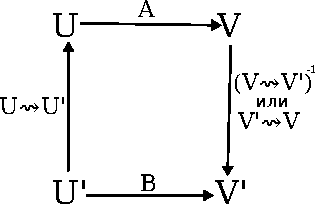
\includegraphics[scale=0.9]{diagram0}
        \end{center}
    \end{figure}

    \subsection{Двойственность}
    Рассмотрим векторное пространство $V=\ind{}R{^n}$.
    Как определено ранее, $V^{*} = \ind{^n}R{} = \Hom(V,R)$ --- двойственный модуль.

    Заметим, что $V \cong V^{*}$ (столбцы на строки меняем): $\vect{x_{1}\\\vdots\\x_{n}} \mapsto \vect{x_{1} & \cdots & x_{n}}$.
    Данный изоморфизм наблюдается только благодаря коммутативности кольца: раньше мы домножали строку слева на матрицу справа;\ теперь мы домножаем транспонированную матрицу слева на столбец справа в двойственном модуле.

    Так как умножение переворачивается, то двойственный левому модулю -- правый, и наоборот.
    Но из-за коммутативности кольца можно утверждать наличие изоморфизма.

    Рассмотрим $(V^*)^*$ --- двойственный двойственному модуль.
    \theorem{
        Между $V$ и $V^{**}$ имеется канонический изоморфизм, не зависящий от выбора базиса.
        \provehere{
            Определим отображение из $V$ в $V^{**}$ так:
            сопоставим вектору $u \in V$ функционал $\theta_u = u^{**} \in V^{**}$.

            Этот функционал при применении справа к любому отображению $\phi \in V^*$, даёт значение отображения в точке $u$:
            \[V^* \times V^{**} \map R;\qquad (\phi)u^{**} = \phi(u)\]

            Теперь заметим, что данное отображение $u \mapsto u^{**}$:
            \bullets{
                \item Действительно не зависит от выбора базиса: он просто не участвует в определении.
                \item Корректно: $u^{**} \in V^{**}$, то есть линейно относительно канонического спаривания с элементами из $V^*$. А именно, аддитивно
                \[        \forall \phi, \psi \in V^*, u^{**} \in V^{**}: \qquad (\phi + \psi)u^{**} = (\phi + \psi)(u) = \phi(u) + \psi(u) = (\phi)u^{**} + (\psi)u^{**}\]
                и однородно
                \[\forall \phi \in V^*, u^{**} \in V^{**}, \lambda \in R: \qquad (\lambda \phi)u^{**} = \lambda \phi(u) = \lambda \cdot (\phi)u^{**}\]

                \item Само по себе --- линейное отображение, то есть аддитивно
                \[\forall \phi \in V^{**}, u, v \in V: \qquad (\phi)(u + v)^{**} = \phi(u + v) = \phi(u) + \phi(v) = (\phi)u^{**} + (\phi)v^{**}\]
                и согласовано с умножением на скаляр
                \[\forall \phi \in V^{**}, u \in V, \lambda \in R: (\phi)(u \lambda)^{**} = \phi(u \lambda) = \phi(u) \lambda = (\phi)u^{**}\cdot \lambda\]
                \item Инъективно. Здесь мы докажем, что $\Ker(u \mapsto u^{**}) = \{0\}$:
                \[u^{**} = 0 \then \forall \phi \in V^*: (\phi)u^{**} = \phi(u) = 0 \then u = 0\]
                \item В конечномерном случае это --- изоморфизм, так как переводит произвольный базис $\{u_1, \dots, u_n\}$ в базис дважды двойственного пространства $\{u_1^{**}, \dots, u_n^{**}\}$.
                В самом деле, $\{u_1^{**}, \dots, u_n^{**}\}$ --- базис, так как $u_i^{**} = (u_i^*)^*$:\[(u_j^*)u_i^{**} = u_j^{*}(u_i) = \delta_{i,j}\cdot 1_R\]
            }
        }
    }
    \intfact{В бесконечномерном случае отображение остаётся инъективным, но перестаёт быть сюръективным;\ если $V$ --- бесконечномерно, то $\dim(V^*) > \dim(V)$.}

    \subsection{Перевод линейным отображением одного функционала в другой}
    В данном разделе $R$ необязательно коммутативно, $U, V$ --- правые модули-$R$.
    Так как линейный функционал, как элемент $U^*$ --- по определению элемент $\Hom(U, R)$, то линейные отображения $U \map V$ являются линейными отображениями не только на элементах пространства $V$, но и на функционалах из $V^*$:

    Всякий функционал $\eta \in V^*; \eta: V \map R$ переводится линейным отображением $\phi: U \map V$ в линейный функционал $\theta = \eta \circ \phi: U \map R$ согласно следующей диаграмме:
    % https://q.uiver.app/?q=WzAsMyxbMCwwLCIgVSJdLFsyLDAsIiBWIl0sWzEsMiwiIFIiXSxbMCwxLCJcXHBoaSJdLFsxLDIsIlxcZXRhIl0sWzAsMiwiXFx0aGV0YSIsMl1d
    \[\begin{tikzcd}[ampersand replacement=\&]
    { U} \&\& { V} \\
    \\
    \& { R}
    \arrow["\phi", from=1-1, to=1-3]
    \arrow["\eta", from=1-3, to=3-2]
    \arrow["\theta"', from=1-1, to=3-2]
    \end{tikzcd}\]

    Данное отображение, сопоставляющее функционалу $\eta: V \map R$ функционал $\theta: U \map R$ называется называется \emph{двойственным} к $\phi$ отображением:
    \[\phi^*: V^* \map U^* \qquad \phi^*: \eta \mapsto (\eta)\phi^* = \eta \circ \phi\]

    \subsubsection{Свойства двойственного отображения}
    \emph{Не уверен, было ли это на лекции, но без этих фактов раздел выглядит совсем куцо.}
    \bullets{
        \item $\phi^*$ --- линейное отображение. Проверим аддитивность, применив $(\eta + \theta)\phi^*$ к произвольному $x \in U$:
        \[((\eta + \theta)\phi^*)(x) = ((\eta + \theta)\circ\phi)(x) = (\eta + \theta)(\phi(x)) = \eta(\phi(x)) + \theta(\phi(x)) = (\eta \circ \phi + \theta \circ \phi)(x) = ((\eta)\phi^* + (\theta)\phi^*)(x)\]
        Аналогично проверяется согласованность с умножением на скаляр $\lambda \in R$:
        \[((\lambda\eta)\phi^*)(x) = ((\lambda \eta) \circ \phi)(x) = \lambda \eta (\phi(x)) = \lambda (\eta \circ \phi)(x) = \lambda((\eta)\phi^*)(x)\]
        \item Пусть кольцо $R$ коммутативно;\ пусть $\{e_1, \dots, e_n\}$ --- базис $U$, $\{f_1, \dots, f_m\}$ --- базис $V$.
        Как известно, $\phi$ определяется своими значениями на элементах базиса $e$;\
        Рассмотрим $(x_{i,j})_{i = 1..m,j=1..n}$ --- матрицу $\phi$.
        А именно, $x_{*,j} = [\phi(e_j)]_f$.

        Утверждается, что в таком случае матрица отображения $\phi^*$, выраженная в двойственных базисах $\{f_1^*, \dots, f_m^*\}$ и $\{e_1^*, \dots, e_n^*\}$ равна $x$.
        \provehere{
            Рассмотрим произвольный $u \in U$; ему соответствует $\phi(u) \in V$.

            Из определения матрицы $x$ ($U, V$ --- \textbf{правые} модули) понятно, что \[[u]_e = x \cdot [\phi(u)]_f\] где $[u]_e$ и $[\phi(u)]_f$ --- столбцы разложения соответствующих векторов по соответствующим базисам.

            Теперь рассмотрим \textbf{левые} модули $U^*, V^*$, и соответствующие двойственные базисы $\{e_1^*, \dots, e_n^*\}$ и $\{f_1^*, \dots, f_n^*\}$.

            Элементы двойственных модулей рассматриваем, как соответствующие им строки координат, канонические спаривания $U^* \times U \map R$ и $V^* \times V \map R$ стали умножением строки на столбец.
            Матрицу отображения $\phi^*$ назовём $x^*$, хотя скоро мы увидим, чему она равна на самом деле.

            Теперь для любого $u \in U, \eta \in V^*$: \[((\eta)\phi^*)(u) = \eta(\phi(u))\qquad \then \qquad ([\eta]_{f^*} \cdot x^*) \cdot [u]_{e} = [\eta]_{f^*}\cdot (x \cdot [u]_e)\]
            то есть матрица $\phi^*$ --- это $x^* = x$, что следует просто-напросто из ассоциативности.
        }
        \item $(\phi + \psi)^* = \phi^* + \psi^*$.
        \item $(\lambda\phi)^* = \phi^*\lambda$.
        \item $(\phi\circ\psi)^* = \psi^*\circ\phi^*$.
        \item $\id^*_V = \id_{V^*}$.
        \item $\phi^{**} = \phi$.
    }

    \newlection{22 декабря 2022 г.}


    \section{Случайные факты \emph{не} из линейной алгебры}
    В данной лекции мы отвлечёмся от линейной алгебры, которой посвящён данный раздел, и докажем одну нетривиальную теорему.

    \subsection{Теорема Галуа}
    \lemma{
        $A_{n}$ порождается циклами длины 3.
        \provehere{
            $A_n$ --- подгруппа чётных перестановок в $S_n$, то есть перестановок, порождённых чётным числом транспозиций.
            Отсюда очевидно, что всякий элемент в $S_n$ порождён перестановками вида $(ij)(kl)$, то есть парой транспозиций.

            Для доказательства леммы покажем, что всякая пара транспозиций является произведением 3-циклов.
            Если среди $i,j,k,l$ 3 различных числа, то произведение $(ij)(kl)$ уже является 3-циклом.

            Иначе $(ij)(kl) = (ij)(jk)(jk)(kl) = (ijk)(jkl)$.

            С другой стороны, каждый 3-цикл сам по себе лежит в $A_n$.
        }}
    \lemma{
        Любая перестановка порождается транспозициями: \[S_n = \langle\{(ij)\}\rangle\]
        \provehere{
            Разложим перестановку на произведение независимых циклов и породим каждый цикл следующим образом:
            \[(i_1 i_2 \dots i_k) = (i_1 i_2)\dots(i_{k-2}i_{k-1})(i_{k-1}i_k)\]
        }}
    \lemma{
        Любая перестановка порождается \emph{фундаментальными} транспозициями --- транспозициями соседних элементов: \[S_n = \langle\defset{(ij)}{i + 1 = j}\rangle\]
        \provehere{
            Докажем, что каждая транспозиция порождается фундаментальными.
            Обозначим транспозицию $i$-го и $j$-го элементов $w_{i,j}$.
            Докажем по индукции, что $w_{j,k} \in \langle (i, i + 1) \rangle$.

            \underline{База:} $|j - k| = 1$.

            \underline{Индукционный переход:} $|j - k| > 1$. Найдётся $m$ строго между $j, k$.
            Заметим, что $w_{j,k} = w_{j,m}w_{m,k}w_{j,m}$, что завершает доказательство.\qedhere
            \provehere[Другой способ доказательства.] {
                Применим алгоритм сортировки пузырьком, который за $\bigO(n^2)$ фундаментальных транспозиций поменяет элементы из любого порядка в любой другой.
            }
        }}
    \definition[$k$-транзитивность]{
        Подгруппа $H \le S_n$ является $k$-транзитивной, если \[\forall(i_1,\dots,i_k),(j_1,\dots,j_k)\text{, таких, что все $i$ различны, все $j$ --- тоже различны, } \exists\pi\in H: \all{\pi(i_1) = j_1\\\dots\\\pi(i_k) = j_k}\]
    }
    Так, $S_n$ является $n$-транзитивной, так как допустим любой набор из $n$ чисел внизу табличной записи.

    Неформально говоря, $k$-транзитивность означает, что мы можем переставить любые $k$ чисел в таком порядке, в каком хотим.
    Дальше уже могут начаться проблемы, не на все из оставшихся мест можно поставить все из оставшихся чисел.

    \lemma{ $A_n$ --- $(n-2)$-транзитивна.}

    Любая $\pi \in A_n$ имеет вид $\pi = \left(\begin{array}{ccccc}
                                                   i_1 & \cdots & i_{n-2} & i_{n-1} & i_n \\
                                                   j_1 & \cdots & j_{n-2} & *       & *
    \end{array}\right)$, где вместо <<$*$>> в каком-то [в таком, чтобы итоговая перестановка получилась чётной] порядке стоят $j_{n-1}$ и $j_{n}$.

    \theorem[Галуа о простоте $A_n$]{\label{Galois_theorem}
    $A_n$ при $n\ge 5$ проста.

    \provehere{ Пусть $H\normeq A_n$. $|A_n|\ge 60 \Rightarrow A_n \neq \{\id\}.$

        Если $H\neq \{\id\}$, то $\exists \pi \in H: \pi \neq \id.$

        <<Потрясающая идея, но её не я придумал>>: прокоммутируем с чем-то маленьким.

        Заметим, что $A_n = \langle(abc)\rangle$. $\pi$ не коммутирует сразу со всеми $(abc)$, иначе $\pi\in\Cent(A_n)$, но $\Cent(A_n) = \{\id\}$ при $n\ge 4$ (в то время, как $A_3$ всё ещё абелева).

        Таким образом, если $\pi\neq\id$, то $\exists(abc):\pi(abc)\neq(abc)\pi$, то есть \[\id \neq \sigma \coloneqq [\pi, (abc)]=\pi(abc)\pi^{-1}(abc)^{-1}\]
        С одной стороны, $\sigma = \pi\left((abc)\pi^{-1}(abc)^{-1}\right)=\pi \circ \ind{^{(abc)}}{\left(\pi^{-1}\right)}{}\in H$.

        С другой стороны, $\sigma = \left(\pi(abc)\pi^{-1}\right)(abc)^{-1}=\ind{^\pi}{(abc)}{}\circ(abc)^{-1}$, то есть произведение двух 3-циклов; назовём $\sigma = (ijh)(klm)$.

        Сколько букв среди этих шести представляют собой различные значения? ${3\le t\coloneqq \left|\left\{i, j, h, k, l, m\right\}\right| \le 6}$.

        Проведём перебор в поисках 3-цикла в $H$:
        \bullets{
            \item $t = 3$: $\sigma$ --- 3-цикл, $\sigma \in H$, 3-цикл нашёлся.

            \item $t = 4$:

            \numbers{
                \item[$1^\circ$]  $\sigma = (ijh)(jhk)=(ij)(hk)$ --- произведение двух транспозиций.
                Именно здесь появляется Vierergruppe как нормальная подгруппа в $A_4$.
                Разберёмся с этим случаем позже.

                \item[$2^\circ$] $\sigma = (ijh)(jkh) = (ijk)(h) = (ijk)$ --- 3-цикл нашёлся.
            }

            \item $t = 5$: $\sigma = (ijh)(hkl)=(ihjkl)$ --- 5-цикл (приведём к 3-циклу позже).

            \item $t = 6$: $\sigma = (ijh)(klm)$. Прокоммутируем: \[[\sigma, (hkl)]=(ijh)(klm)(hkl)(kml)(ijh)(hlk)=(ilkhm)(j) = (ilkhm)\]
            Опять же, получили 5-цикл.

        }\ok
        Разбираемся с 5-циклами.

        Прокоммутируем, мы же уже поняли, что получается что-то из $H$ и полюбили коммутаторы, да? Ну, вот:
        \[[(ijhkl), (ijh)] = (ijhkl)(ijh)(lkhji)(hji)=(ikj)(h)(l) = (ijk)\]
        \ok
        Разбираемся со случаем $1^\circ$ при $t = 4$.

        Что мы делаем? Правильно:

        \[[(ij)(hk),(hkl)]=(ij)(hk)(hkl)(hk)(ij)(hlk)=(i)(j)(hkl) = (hkl)\]

        Заметим, что здесь нам понадобилась буква $l$, которой там не было, то есть всего различных букв должно быть хотя бы $5$.
        То есть необходимое условие состоит в том, что $n\ge 5$.

        Интересно заметить, что это единственное место, которое не работает при $n = 4$.
        В самом деле, $V = \{\id, (12)(34), (13)(24), (14)(23)\}$ --- нормальная подгруппа (причём не только в $A_4$, но даже и в $S_4$).

        \ok
        Таким образом при $n\ge 5$ в любой нормальной нетривиальной ($\ne \{\id\}$) подгруппе существует 3-цикл.

        В силу $(n-2)$-транзитивности (а $n-2\ge 3$, пам-пам!) в $H$ содержатся \textbf{все} 3-циклы $\then H\ge A_n \Rightarrow H = A_n$: данный 3-цикл можно так сопрячь, чтобы получился другой 3-цикл, в силу $(n-2)$-транзитивности сопрягающая перестановка лежит в $A_n$.
    }
    }

    \subsection{Колокола в Англии}
    В Англии всего 8 колоколов, причём они звонят очень хитрым образом.

    Сначала они звонят в порядке $[1, 2, \dots, 8]$, а потом служители меняют какую-то пару из них.
    После этого они звонят в новом порядке, и так далее.

    В итоге все $8! = 40320$ перестановок обзваниваются по одному разу.

    Может ли быть такое (и как)?
    \provehere{
        Нарисуем граф, неориентированное ребро проходит между двумя перестановками $\pi$ и $\sigma$, такими, что $\pi = (ij)\sigma$ для некоторых $i, j$.

        Докажем,что при $n \geq 3$ для любой пары перестановок $\pi$, $\sigma$ разной чётности существует гамильтонов путь из одной в другую.

        Заметим, что условие достаточно проверять только для одной из перестановок, равной $\id$ (домножение всех перестановок --- вершин в графе --- на фиксированную перестановку $\alpha$ сохраняет рёбра, \emph{изоморфизм графа}, если позволите).

        Будем действовать по индукции.

        \underline{База:} $n = 2$. В графе $2$ перестановки, между ними есть ребро.

        \underline{Переход:} $n \ge 3$.
        Зафиксируем некий индекс $i$, такой, что $\pi_i \ne \sigma_i$.
        Перечислим в некотором порядке числа $1..n$ так, чтобы первым оказалось число $\pi_i$, а последним --- число $\sigma_i$.

        Будем по очереди перебирать перестановки в графе, составляя путь, так, чтобы сначала пройти по всем перестановкам $\beta: \beta_i = \pi_i$, потом --- по всем перестановкам $\beta: \beta_i$ --- второе число из списка, и так далее.

        Так как $n!$ чётно, то действительно путь будет вести из перестановки одной чётности в перестановку другой чётности.
        Внутри частей пути $\{\beta_j\}_{j = 1}^{n!}$ с фиксированным $\beta_i$ путь строится по индукции, вне частей $\beta_i$ меняется так, чтобы стать следующим числом в списке.
    }
\end{document}
